\ifnpas

\begin{figure}[htbp]
\centering
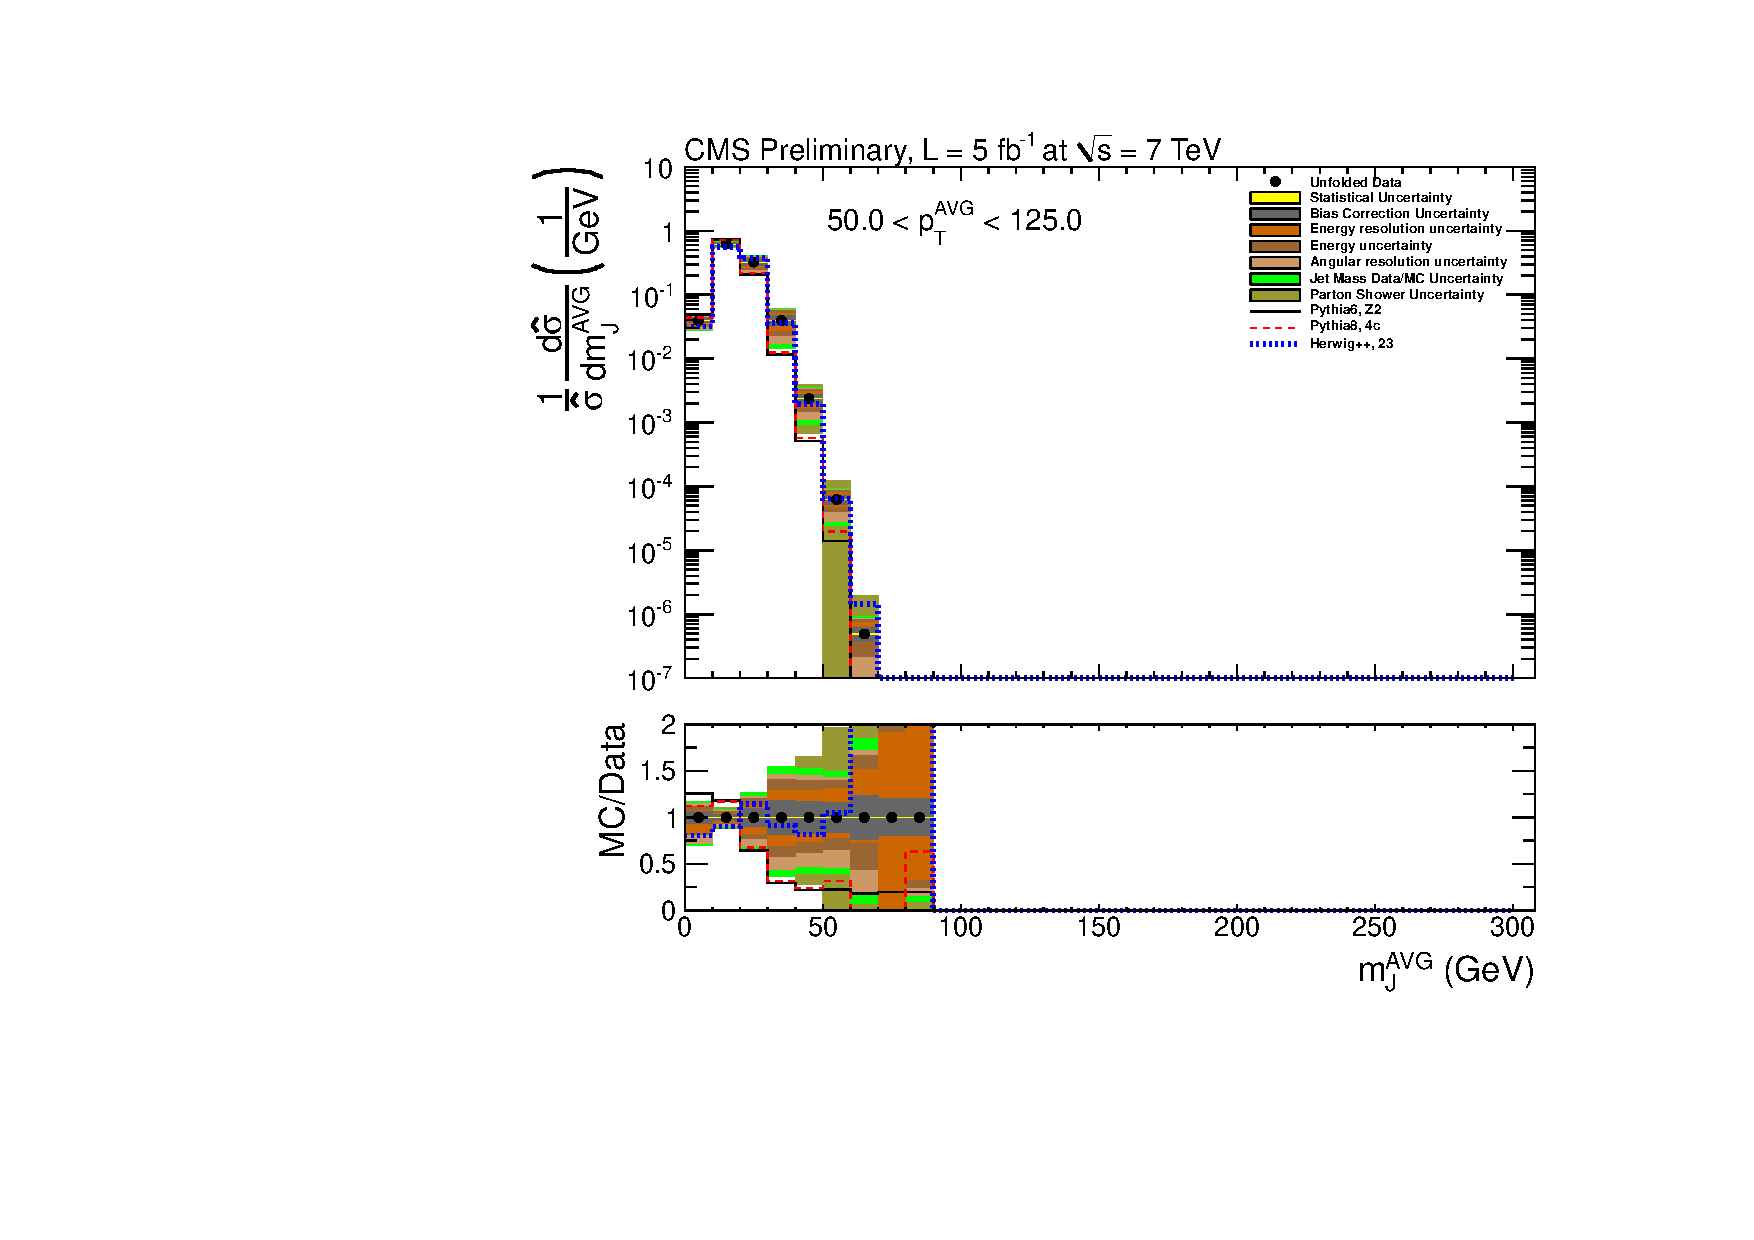
\includegraphics[width=0.95\textwidth]{figs/unfoldedMeasurementDijets_1_allsys}
\caption{Unfolded distributions of the jet mass for AK7 jets,
for $50.0 < \pt^{AVG} < 125.0$ \GeVc. The data are shown in black
points. 
The statistical uncertainty is shown in light yellow, the uncertainties due to the jet-energy resolution, jet-energy scale, and jet-angular resolution are shown in shades of brown, the uncertainty due to pile-up is shown in green, and the uncertainty due to the parton shower are shown in dark yellow.
The simulated distribution from \PYTHIA is shown in solid black, 
the from \PYTHIAEIGHT in dashed red, and from \HERWIG in dotted blue. 
The bottom frame shows the ratio of the true distribution from
the simulation divided by the unfolded distribution, along with
the uncertainties in the unfolded distribution. 
\label{figs:unfoldedMeasurementDijets_1_allsys}}
\end{figure}



\begin{figure}[htbp]
\centering
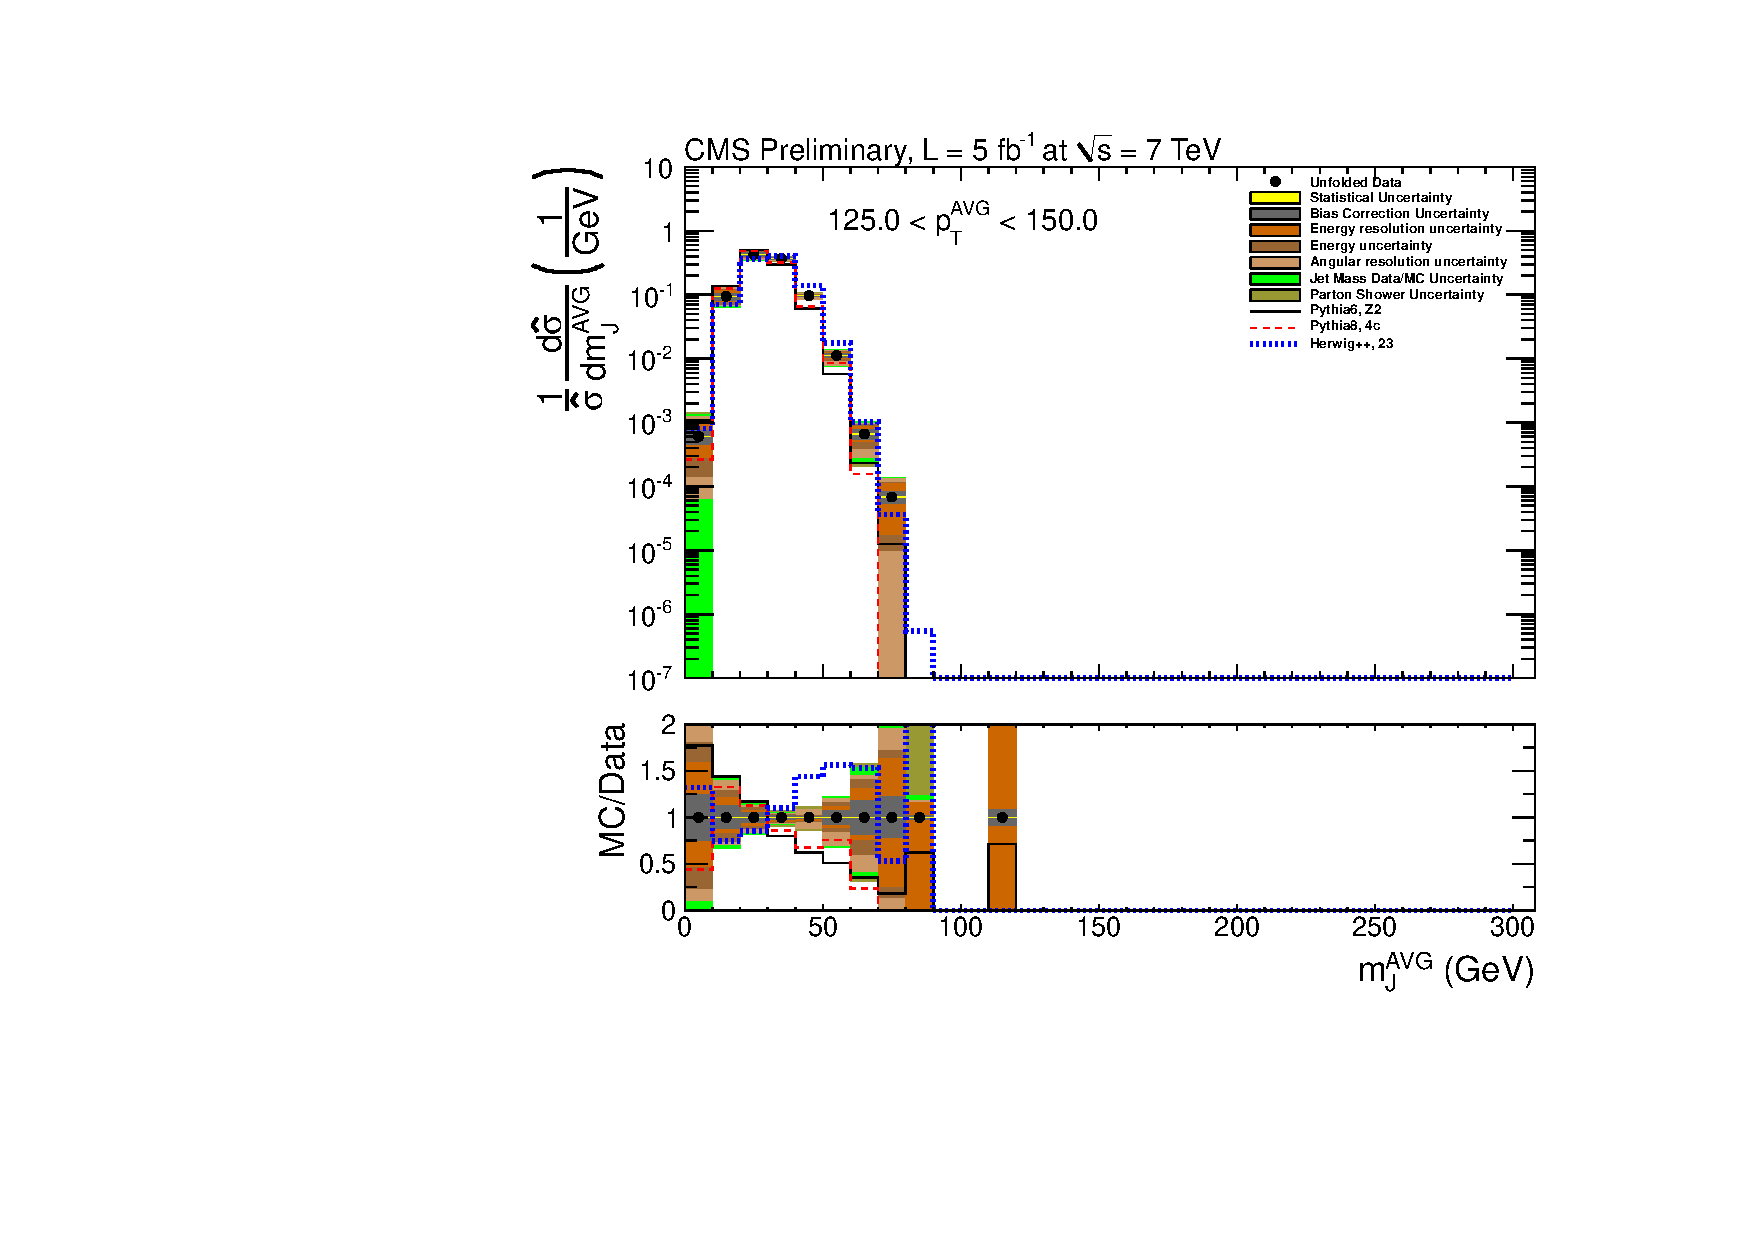
\includegraphics[width=0.95\textwidth]{figs/unfoldedMeasurementDijets_2_allsys}
\caption{Unfolded distributions of the jet mass for AK7 jets,
for $125.0 < \pt^{AVG} < 150.0$ \GeVc. The data are shown in black
points. 
The statistical uncertainty is shown in light yellow, the uncertainties due to the jet-energy resolution, jet-energy scale, and jet-angular resolution are shown in shades of brown, the uncertainty due to pile-up is shown in green, and the uncertainty due to the parton shower are shown in dark yellow.
The simulated distribution from \PYTHIA is shown in solid black, 
the from \PYTHIAEIGHT in dashed red, and from \HERWIG in dotted blue. 
The bottom frame shows the ratio of the true distribution from
the simulation divided by the unfolded distribution, along with
the uncertainties in the unfolded distribution. 
\label{figs:unfoldedMeasurementDijets_2_allsys}}
\end{figure}



\begin{figure}[htbp]
\centering
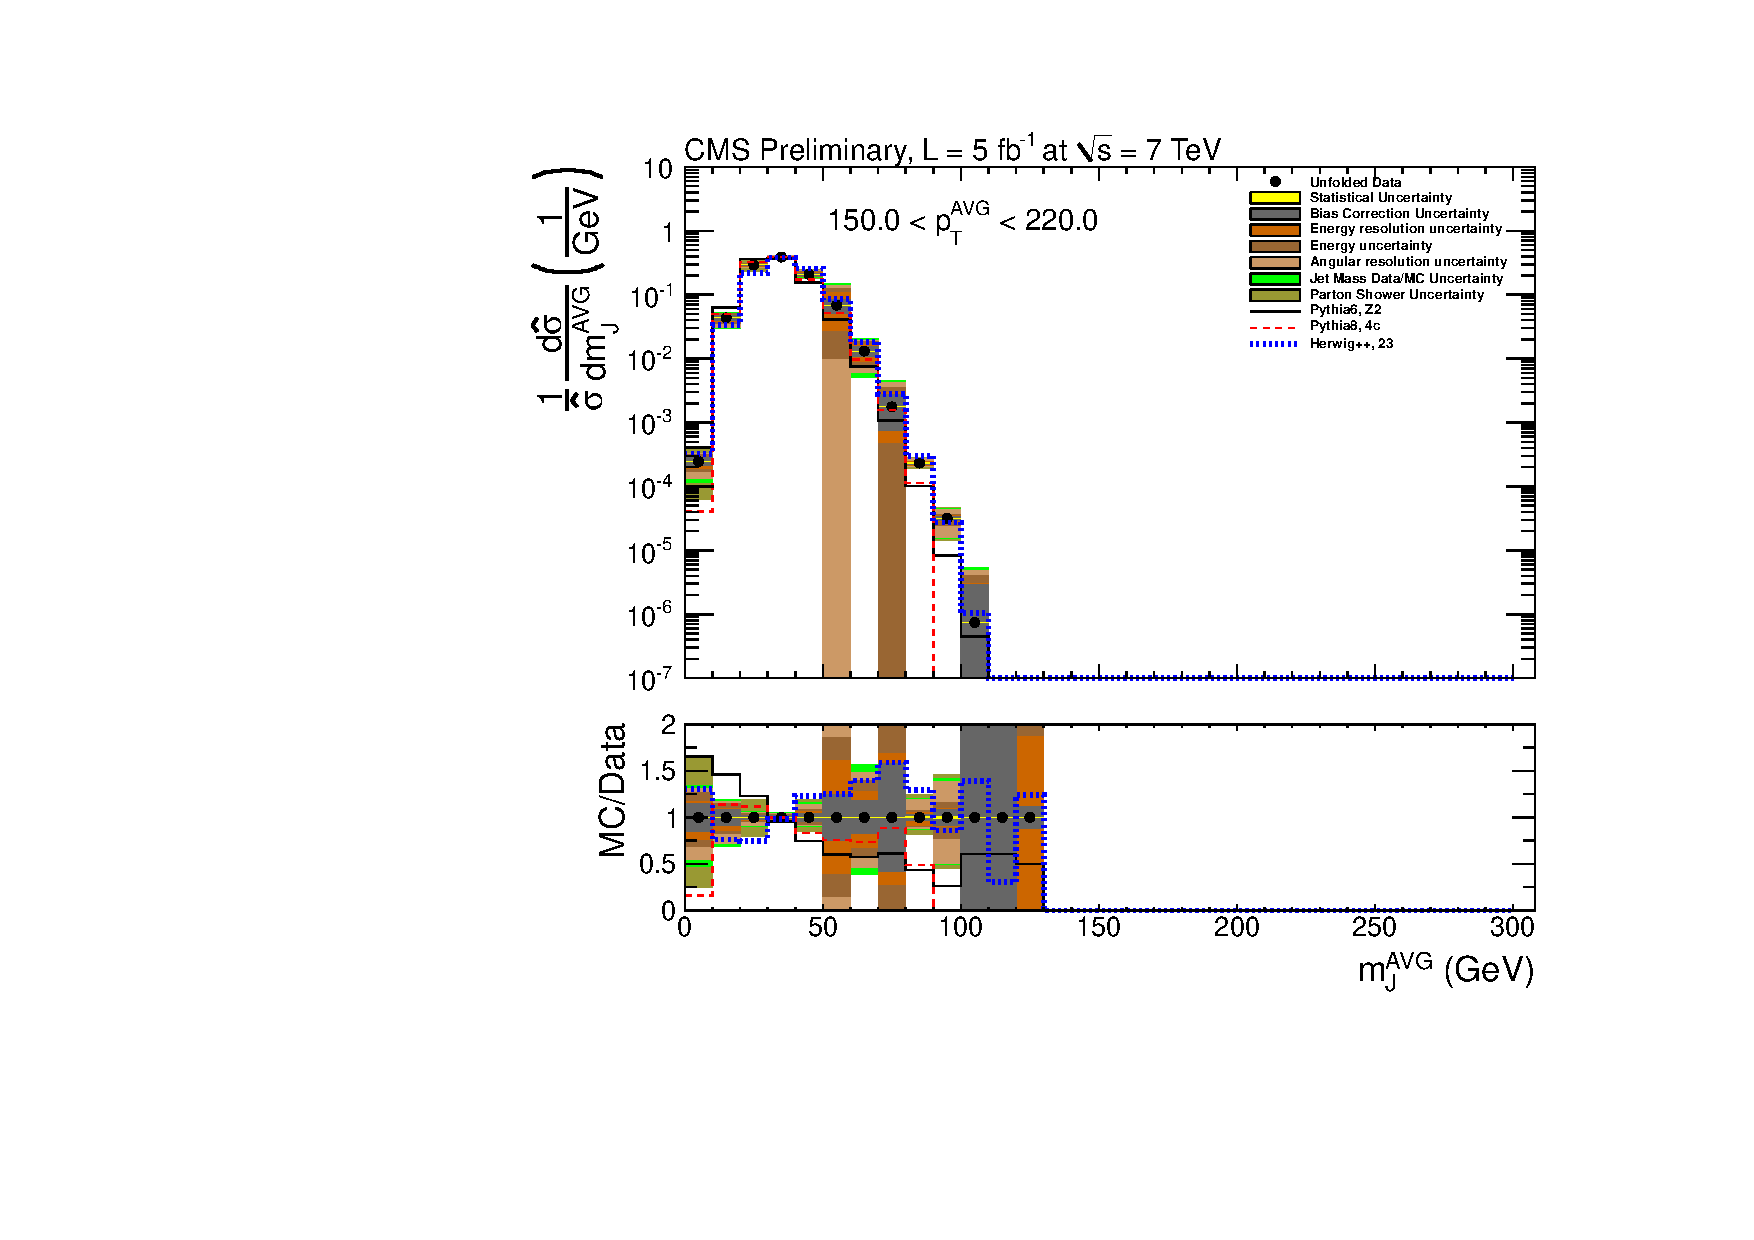
\includegraphics[width=0.95\textwidth]{figs/unfoldedMeasurementDijets_3_allsys}
\caption{Unfolded distributions of the jet mass for AK7 jets,
for $150.0 < \pt^{AVG} < 220.0$ \GeVc. The data are shown in black
points. 
The statistical uncertainty is shown in light yellow, the uncertainties due to the jet-energy resolution, jet-energy scale, and jet-angular resolution are shown in shades of brown, the uncertainty due to pile-up is shown in green, and the uncertainty due to the parton shower are shown in dark yellow.
The simulated distribution from \PYTHIA is shown in solid black, 
the from \PYTHIAEIGHT in dashed red, and from \HERWIG in dotted blue. 
The bottom frame shows the ratio of the true distribution from
the simulation divided by the unfolded distribution, along with
the uncertainties in the unfolded distribution. 
\label{figs:unfoldedMeasurementDijets_3_allsys}}
\end{figure}



\begin{figure}[htbp]
\centering
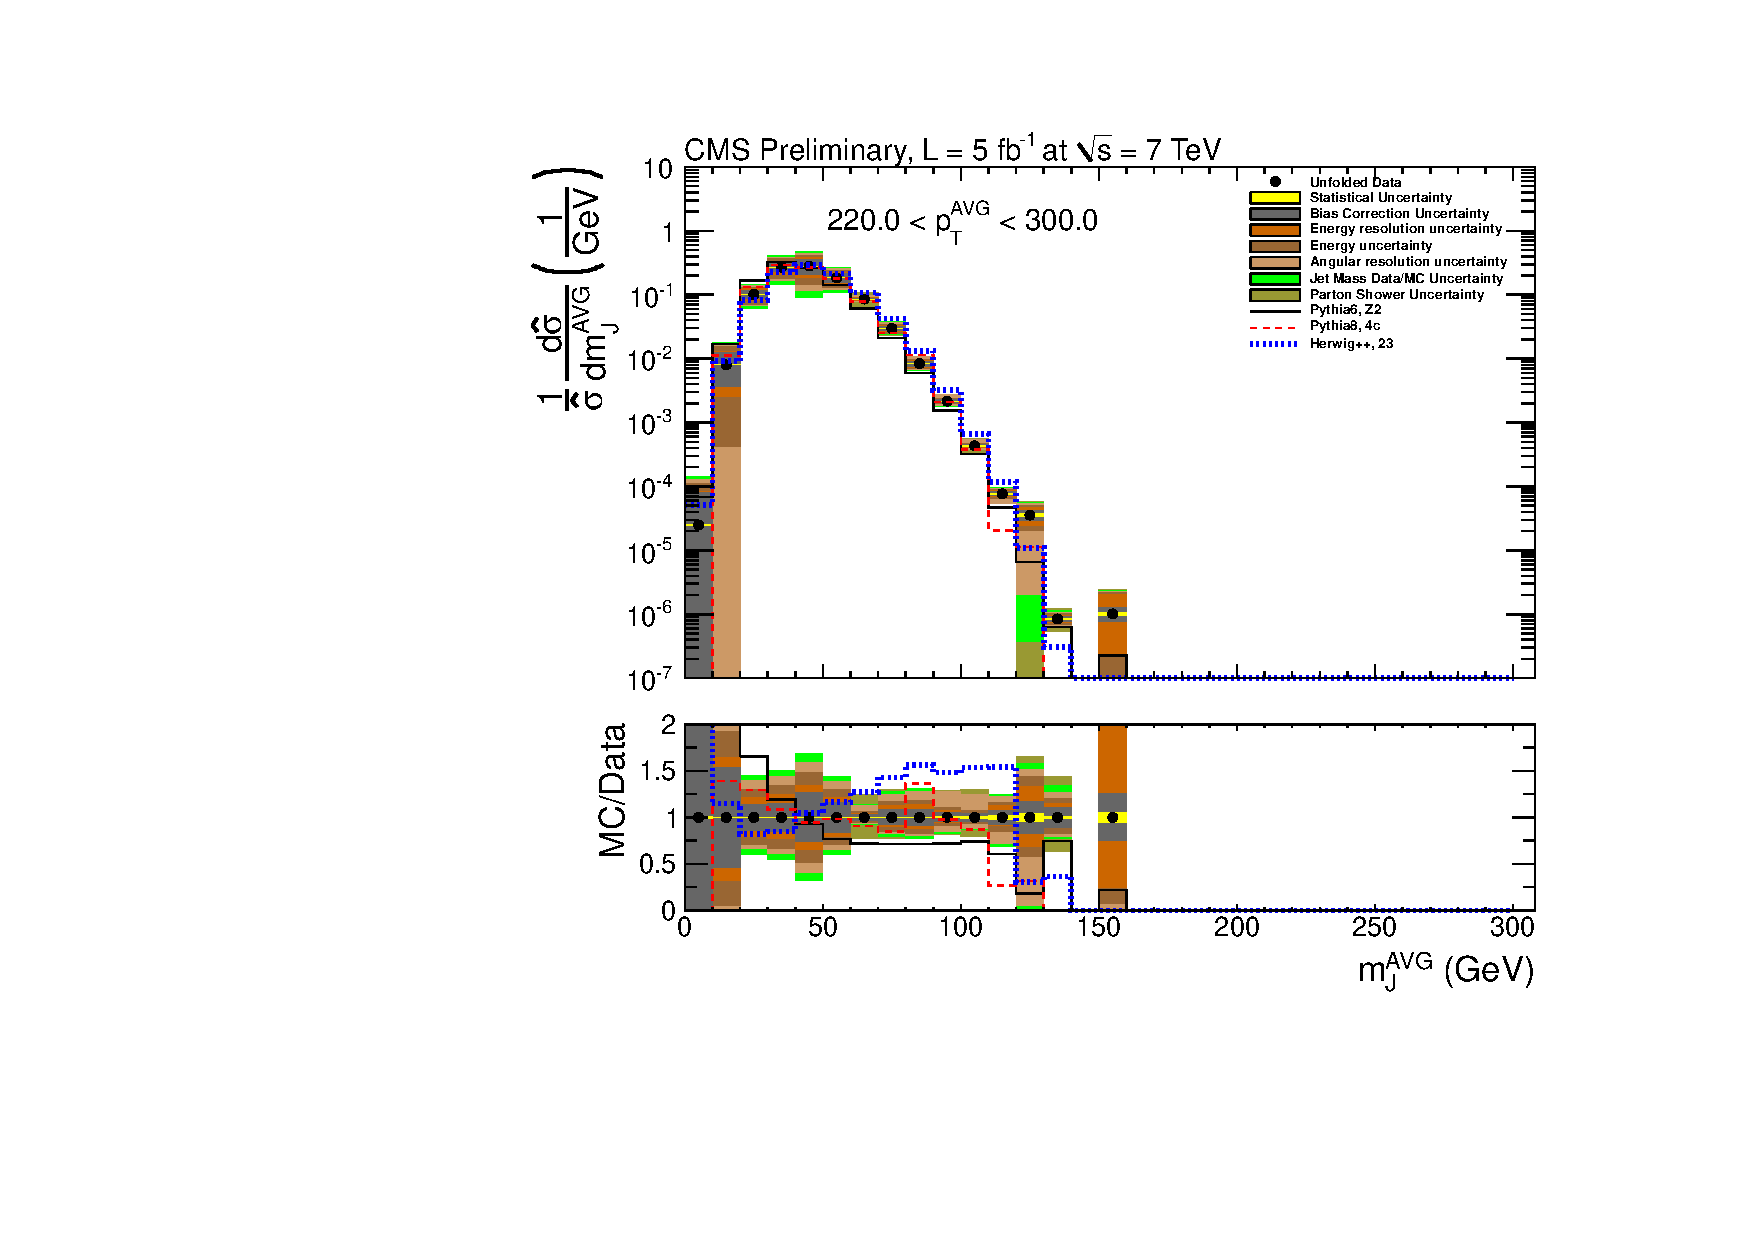
\includegraphics[width=0.95\textwidth]{figs/unfoldedMeasurementDijets_4_allsys}
\caption{Unfolded distributions of the jet mass for AK7 jets,
for $220.0 < \pt^{AVG} < 300.0$ \GeVc. The data are shown in black
points. 
The statistical uncertainty is shown in light yellow, the uncertainties due to the jet-energy resolution, jet-energy scale, and jet-angular resolution are shown in shades of brown, the uncertainty due to pile-up is shown in green, and the uncertainty due to the parton shower are shown in dark yellow.
The simulated distribution from \PYTHIA is shown in solid black, 
the from \PYTHIAEIGHT in dashed red, and from \HERWIG in dotted blue. 
The bottom frame shows the ratio of the true distribution from
the simulation divided by the unfolded distribution, along with
the uncertainties in the unfolded distribution. 
\label{figs:unfoldedMeasurementDijets_4_allsys}}
\end{figure}



\begin{figure}[htbp]
\centering
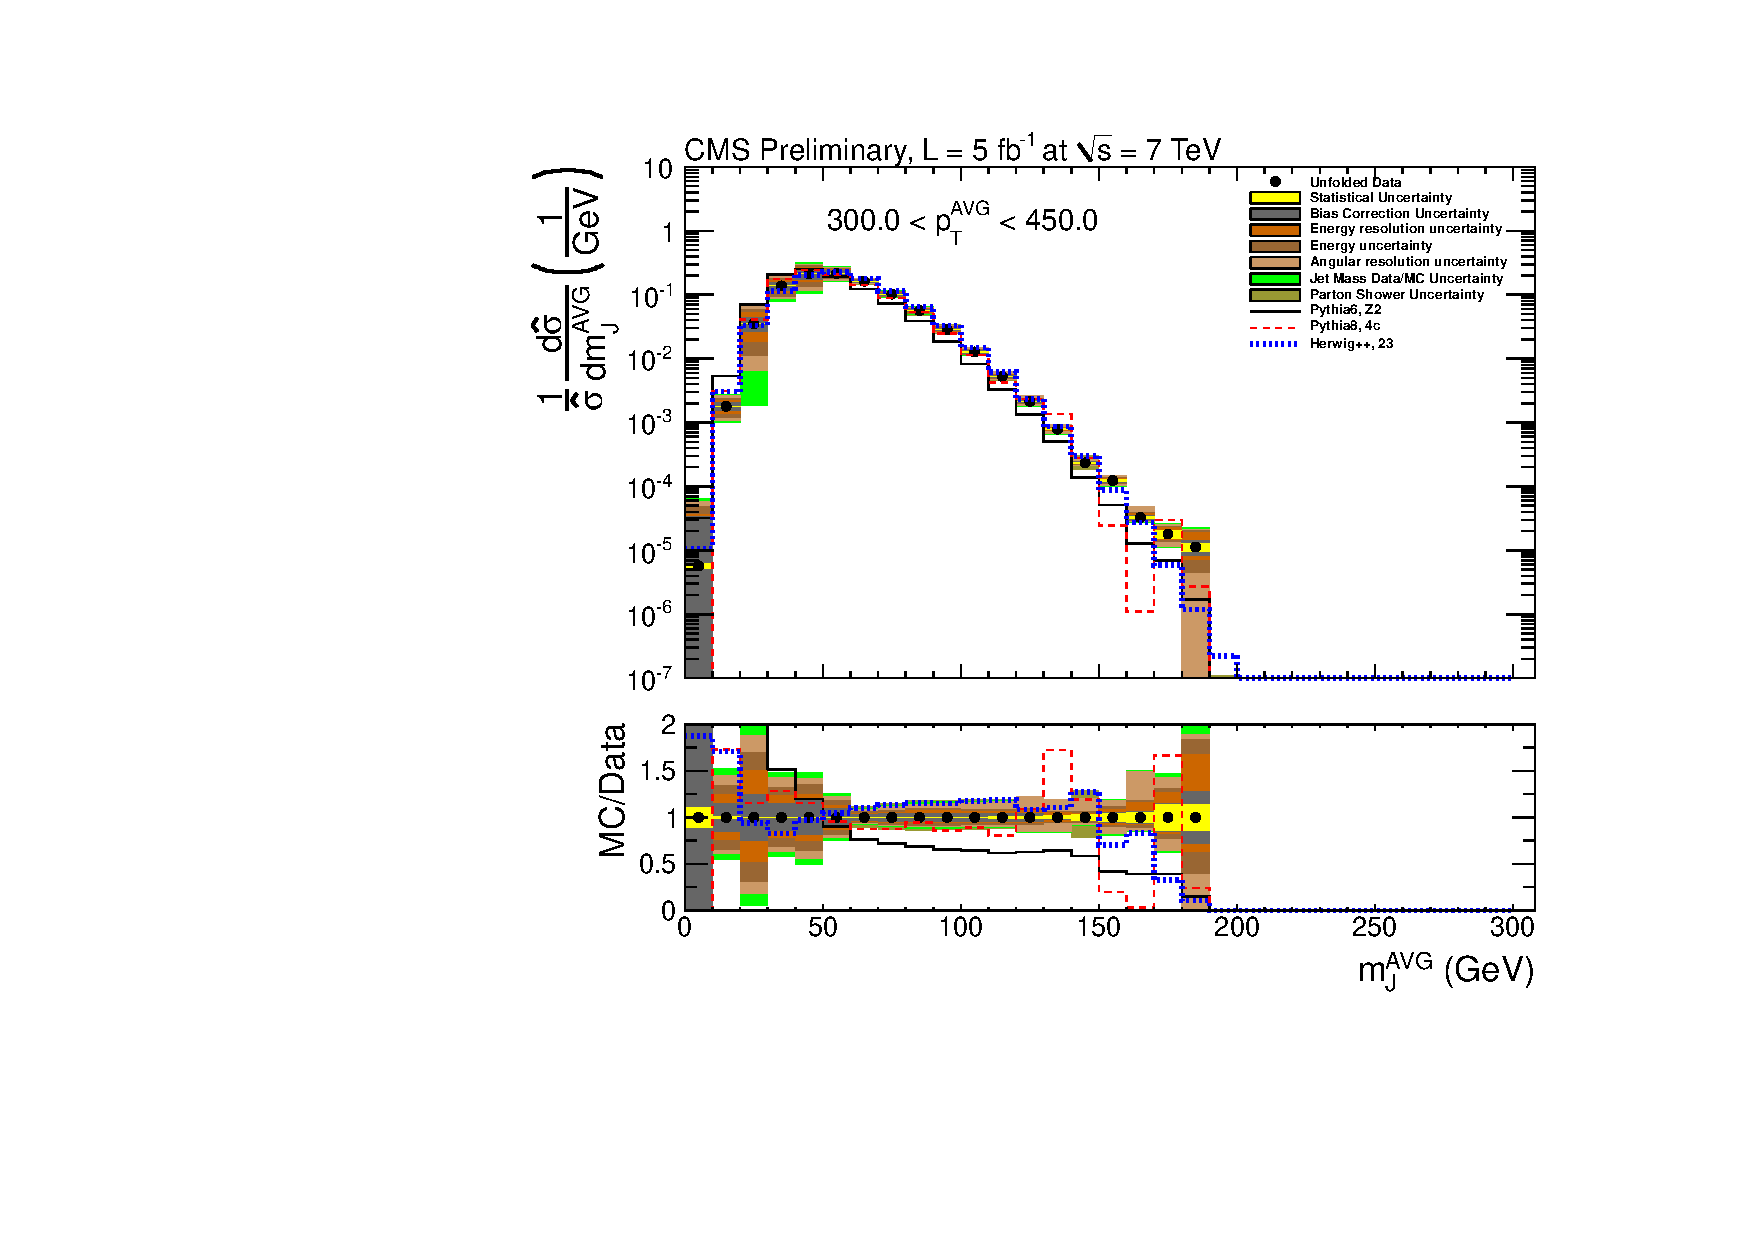
\includegraphics[width=0.95\textwidth]{figs/unfoldedMeasurementDijets_5_allsys}
\caption{Unfolded distributions of the jet mass for AK7 jets,
for $300.0 < \pt^{AVG} < 450.0$ \GeVc. The data are shown in black
points. 
The statistical uncertainty is shown in light yellow, the uncertainties due to the jet-energy resolution, jet-energy scale, and jet-angular resolution are shown in shades of brown, the uncertainty due to pile-up is shown in green, and the uncertainty due to the parton shower are shown in dark yellow.
The simulated distribution from \PYTHIA is shown in solid black, 
the from \PYTHIAEIGHT in dashed red, and from \HERWIG in dotted blue. 
The bottom frame shows the ratio of the true distribution from
the simulation divided by the unfolded distribution, along with
the uncertainties in the unfolded distribution. 
\label{figs:unfoldedMeasurementDijets_5_allsys}}
\end{figure}



\begin{figure}[htbp]
\centering
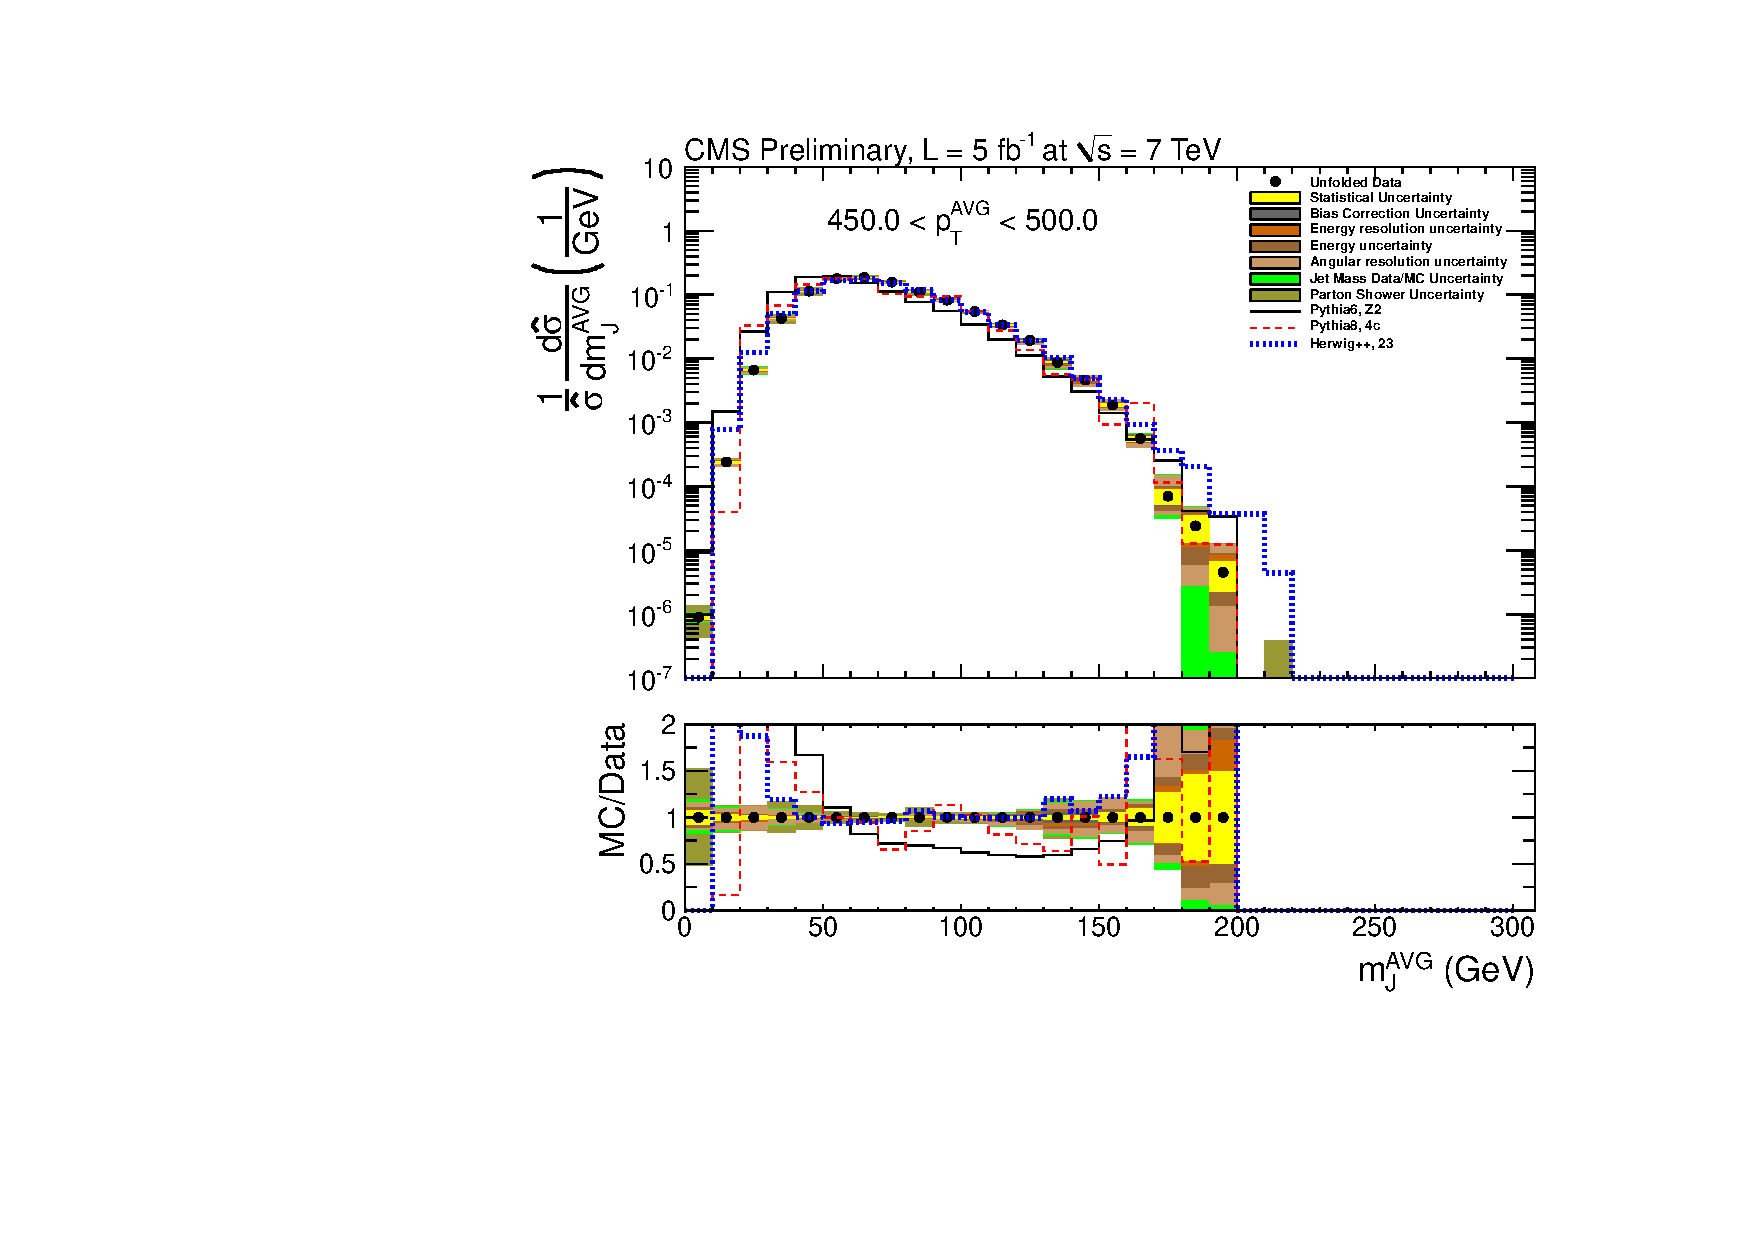
\includegraphics[width=0.95\textwidth]{figs/unfoldedMeasurementDijets_6_allsys}
\caption{Unfolded distributions of the jet mass for AK7 jets,
for $450.0 < \pt^{AVG} < 500.0$ \GeVc. The data are shown in black
points. 
The statistical uncertainty is shown in light yellow, the uncertainties due to the jet-energy resolution, jet-energy scale, and jet-angular resolution are shown in shades of brown, the uncertainty due to pile-up is shown in green, and the uncertainty due to the parton shower are shown in dark yellow.
The simulated distribution from \PYTHIA is shown in solid black, 
the from \PYTHIAEIGHT in dashed red, and from \HERWIG in dotted blue. 
The bottom frame shows the ratio of the true distribution from
the simulation divided by the unfolded distribution, along with
the uncertainties in the unfolded distribution. 
\label{figs:unfoldedMeasurementDijets_6_allsys}}
\end{figure}



\begin{figure}[htbp]
\centering
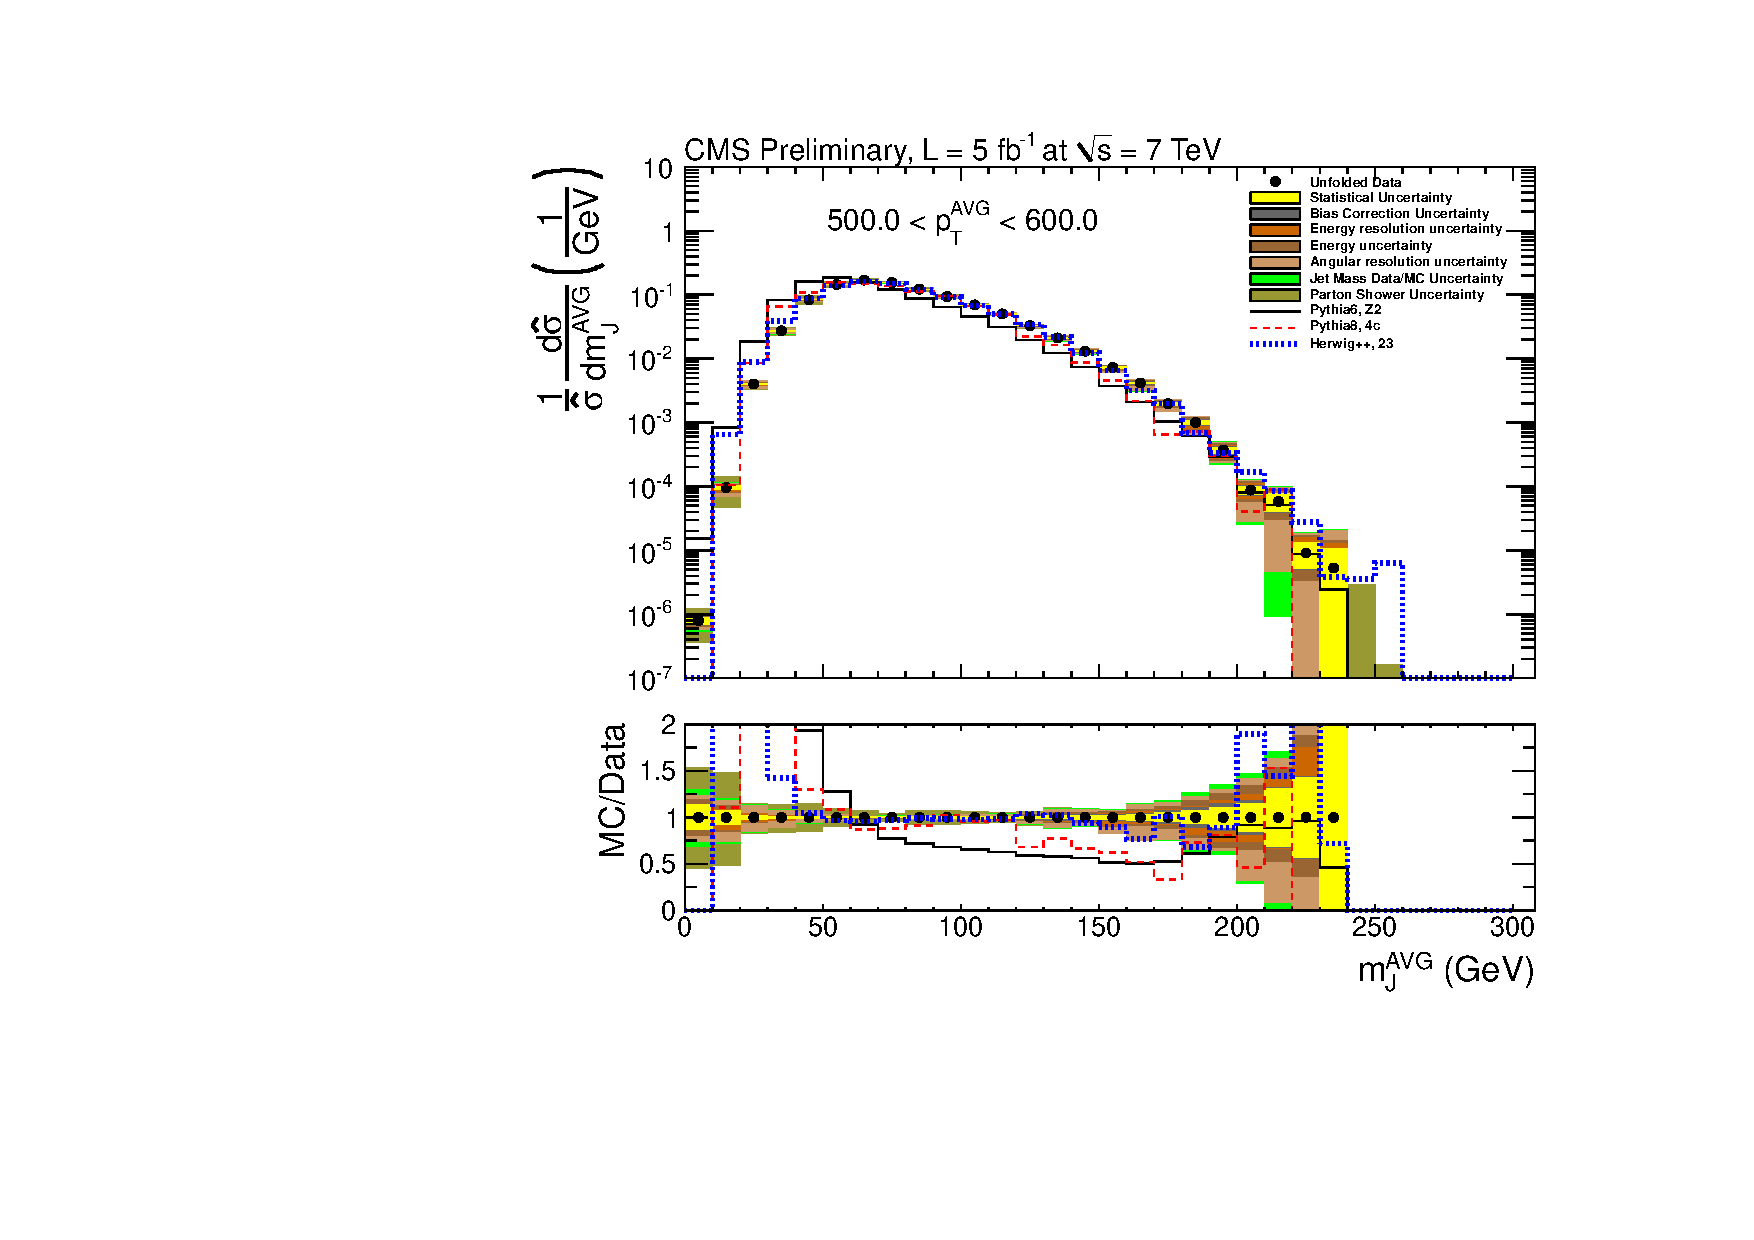
\includegraphics[width=0.95\textwidth]{figs/unfoldedMeasurementDijets_7_allsys}
\caption{Unfolded distributions of the jet mass for AK7 jets,
for $500.0 < \pt^{AVG} < 600.0$ \GeVc. The data are shown in black
points. 
The statistical uncertainty is shown in light yellow, the uncertainties due to the jet-energy resolution, jet-energy scale, and jet-angular resolution are shown in shades of brown, the uncertainty due to pile-up is shown in green, and the uncertainty due to the parton shower are shown in dark yellow.
The simulated distribution from \PYTHIA is shown in solid black, 
the from \PYTHIAEIGHT in dashed red, and from \HERWIG in dotted blue. 
The bottom frame shows the ratio of the true distribution from
the simulation divided by the unfolded distribution, along with
the uncertainties in the unfolded distribution. 
\label{figs:unfoldedMeasurementDijets_7_allsys}}
\end{figure}



\begin{figure}[htbp]
\centering
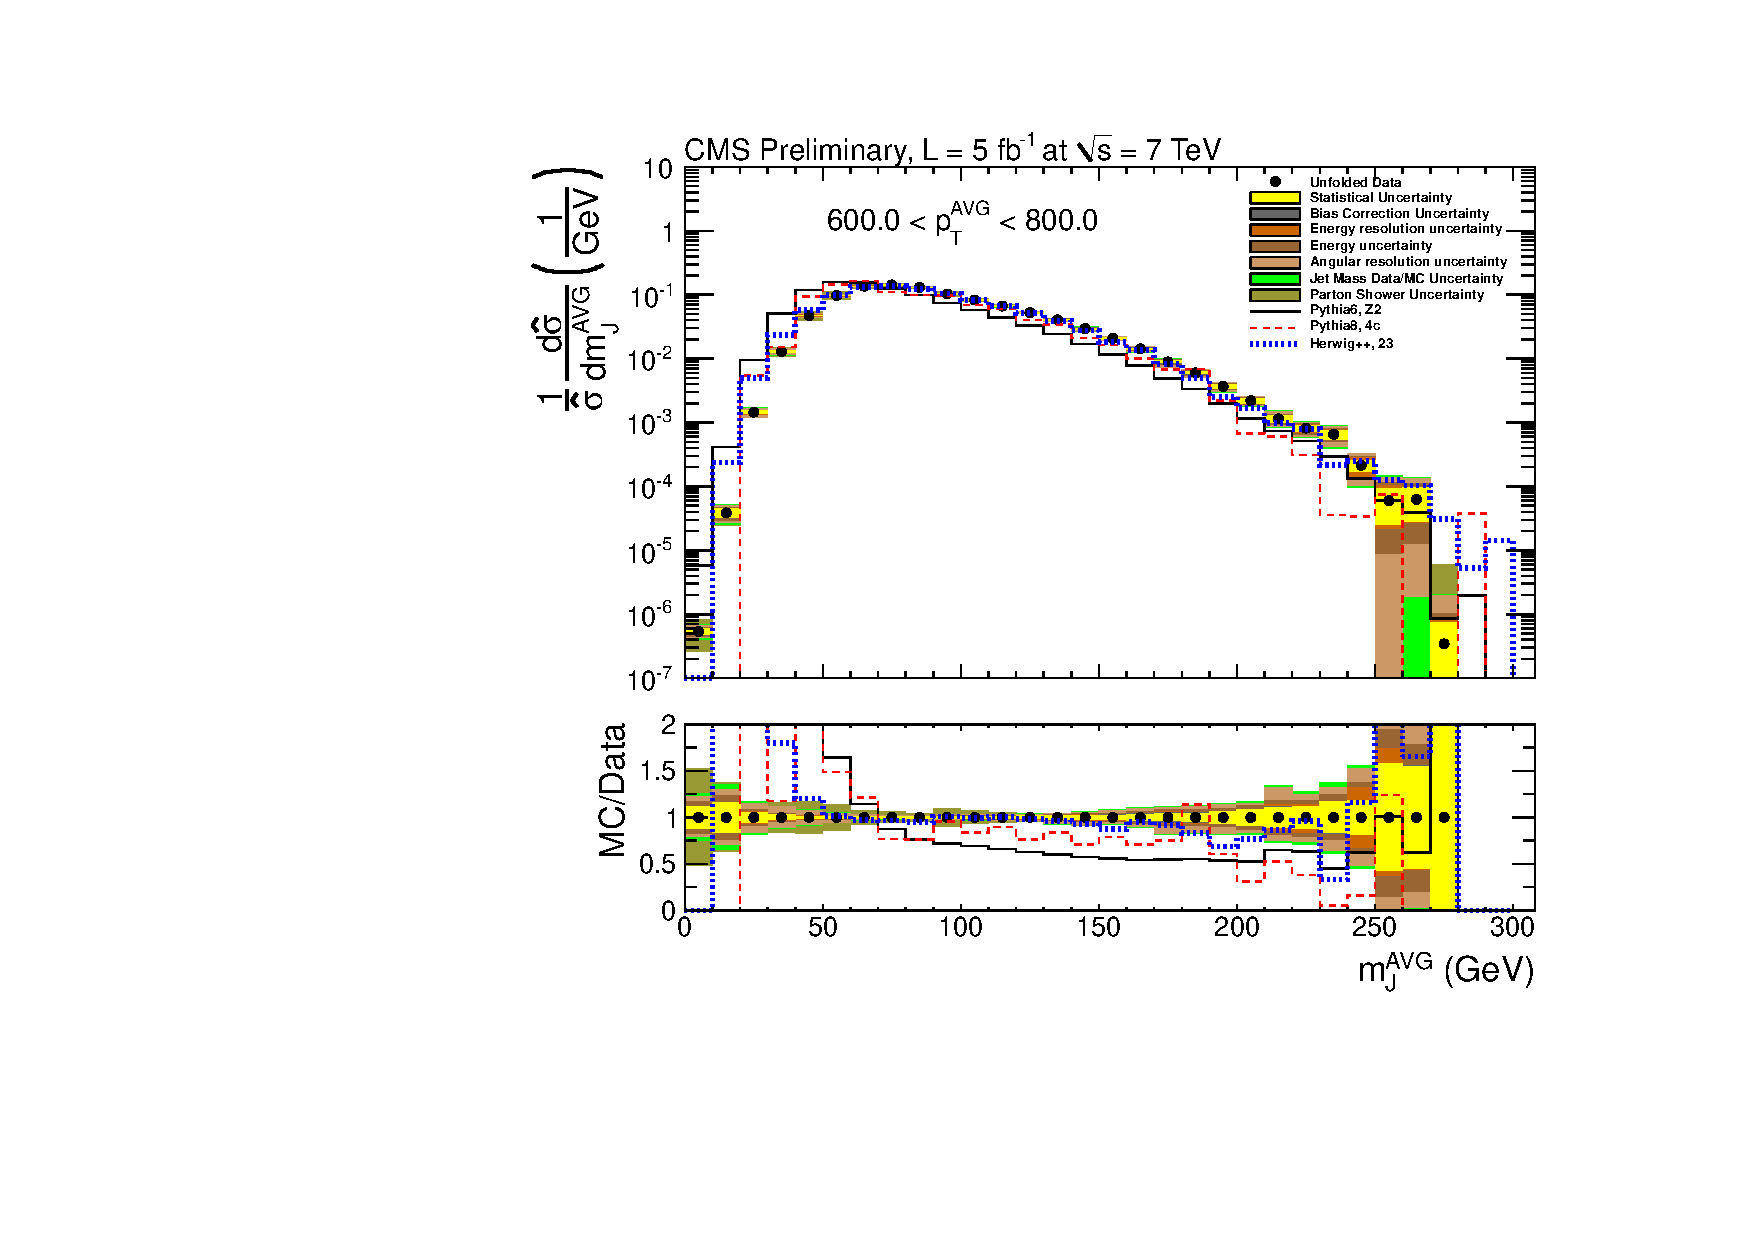
\includegraphics[width=0.95\textwidth]{figs/unfoldedMeasurementDijets_8_allsys}
\caption{Unfolded distributions of the jet mass for AK7 jets,
for $600.0 < \pt^{AVG} < 800.0$ \GeVc. The data are shown in black
points. 
The statistical uncertainty is shown in light yellow, the uncertainties due to the jet-energy resolution, jet-energy scale, and jet-angular resolution are shown in shades of brown, the uncertainty due to pile-up is shown in green, and the uncertainty due to the parton shower are shown in dark yellow.
The simulated distribution from \PYTHIA is shown in solid black, 
the from \PYTHIAEIGHT in dashed red, and from \HERWIG in dotted blue. 
The bottom frame shows the ratio of the true distribution from
the simulation divided by the unfolded distribution, along with
the uncertainties in the unfolded distribution. 
\label{figs:unfoldedMeasurementDijets_8_allsys}}
\end{figure}



\begin{figure}[htbp]
\centering
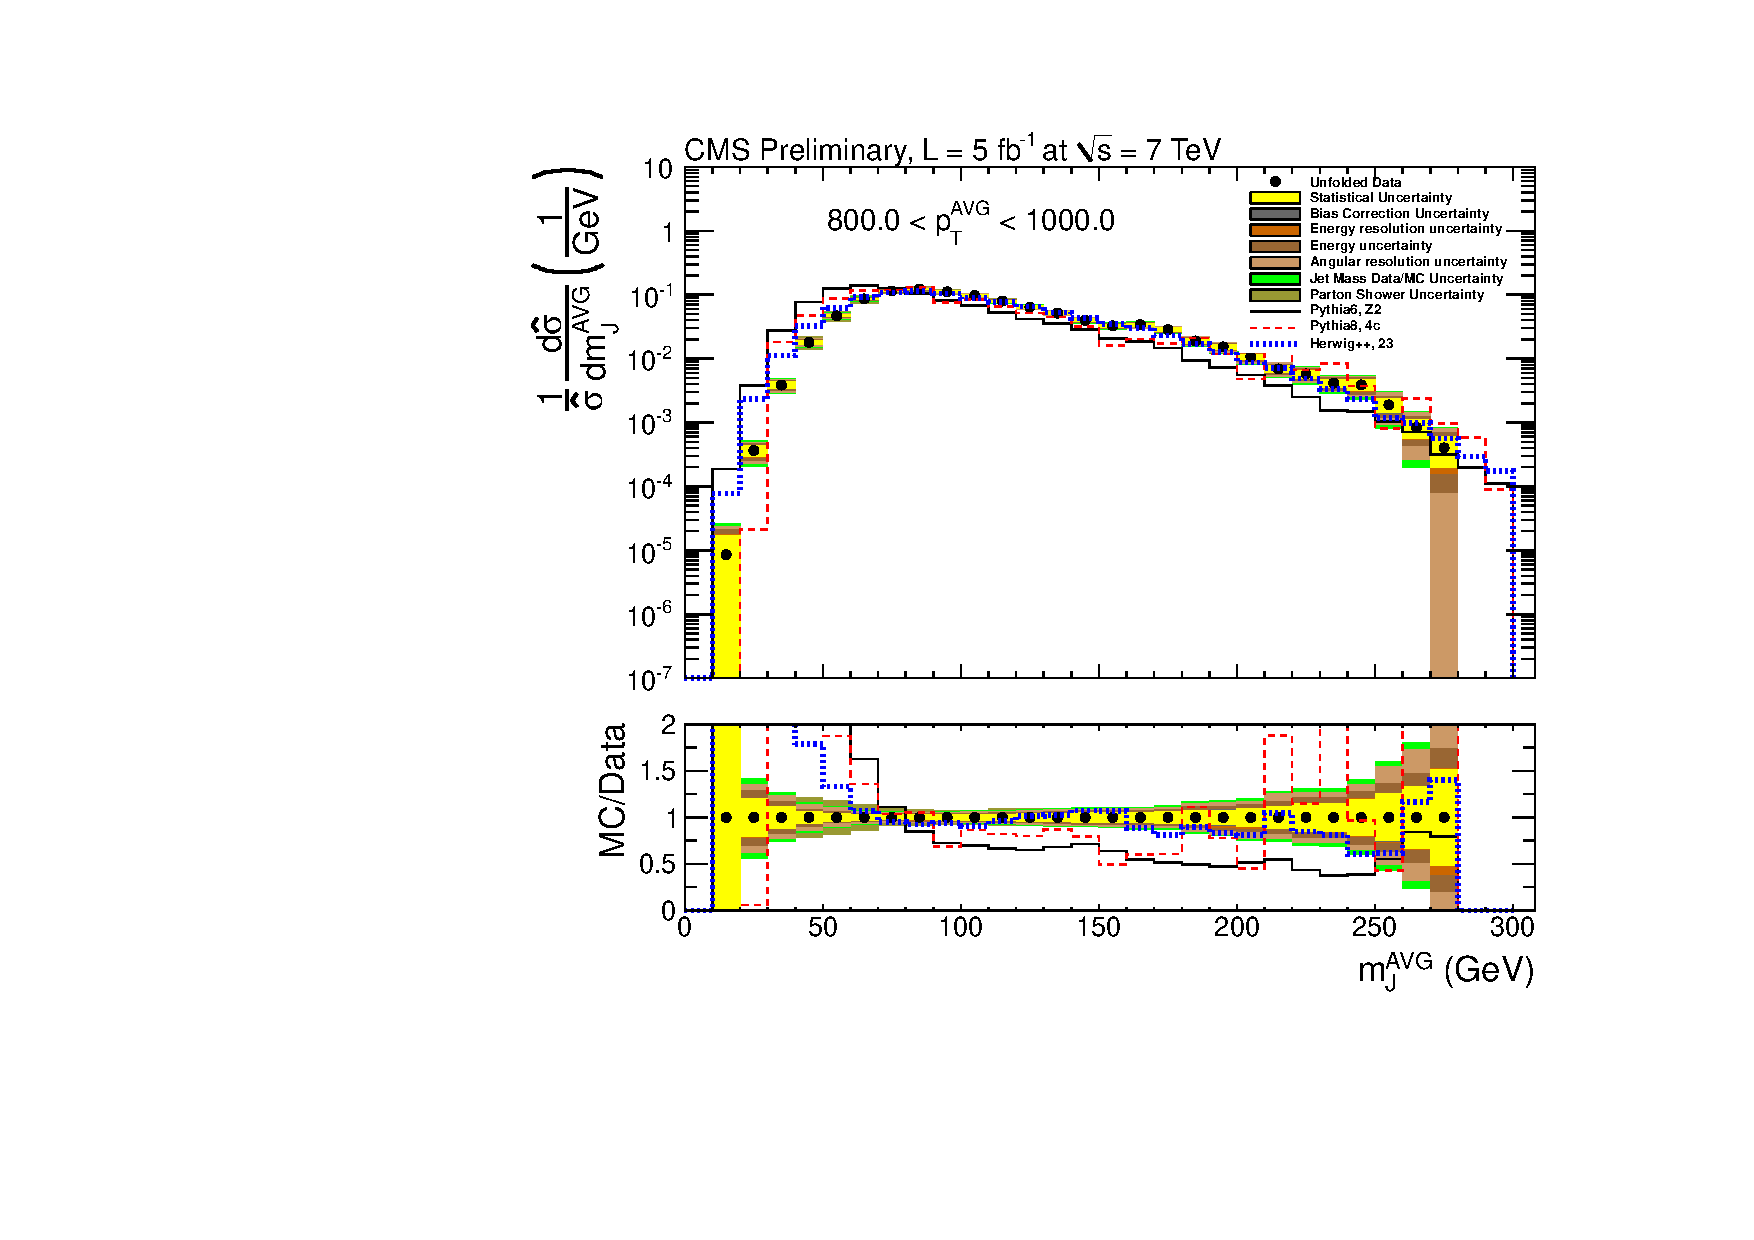
\includegraphics[width=0.95\textwidth]{figs/unfoldedMeasurementDijets_9_allsys}
\caption{Unfolded distributions of the jet mass for AK7 jets,
for $800.0 < \pt^{AVG} < 1000.0$ \GeVc. The data are shown in black
points. 
The statistical uncertainty is shown in light yellow, the uncertainties due to the jet-energy resolution, jet-energy scale, and jet-angular resolution are shown in shades of brown, the uncertainty due to pile-up is shown in green, and the uncertainty due to the parton shower are shown in dark yellow.
The simulated distribution from \PYTHIA is shown in solid black, 
the from \PYTHIAEIGHT in dashed red, and from \HERWIG in dotted blue. 
The bottom frame shows the ratio of the true distribution from
the simulation divided by the unfolded distribution, along with
the uncertainties in the unfolded distribution. 
\label{figs:unfoldedMeasurementDijets_9_allsys}}
\end{figure}



\begin{figure}[htbp]
\centering
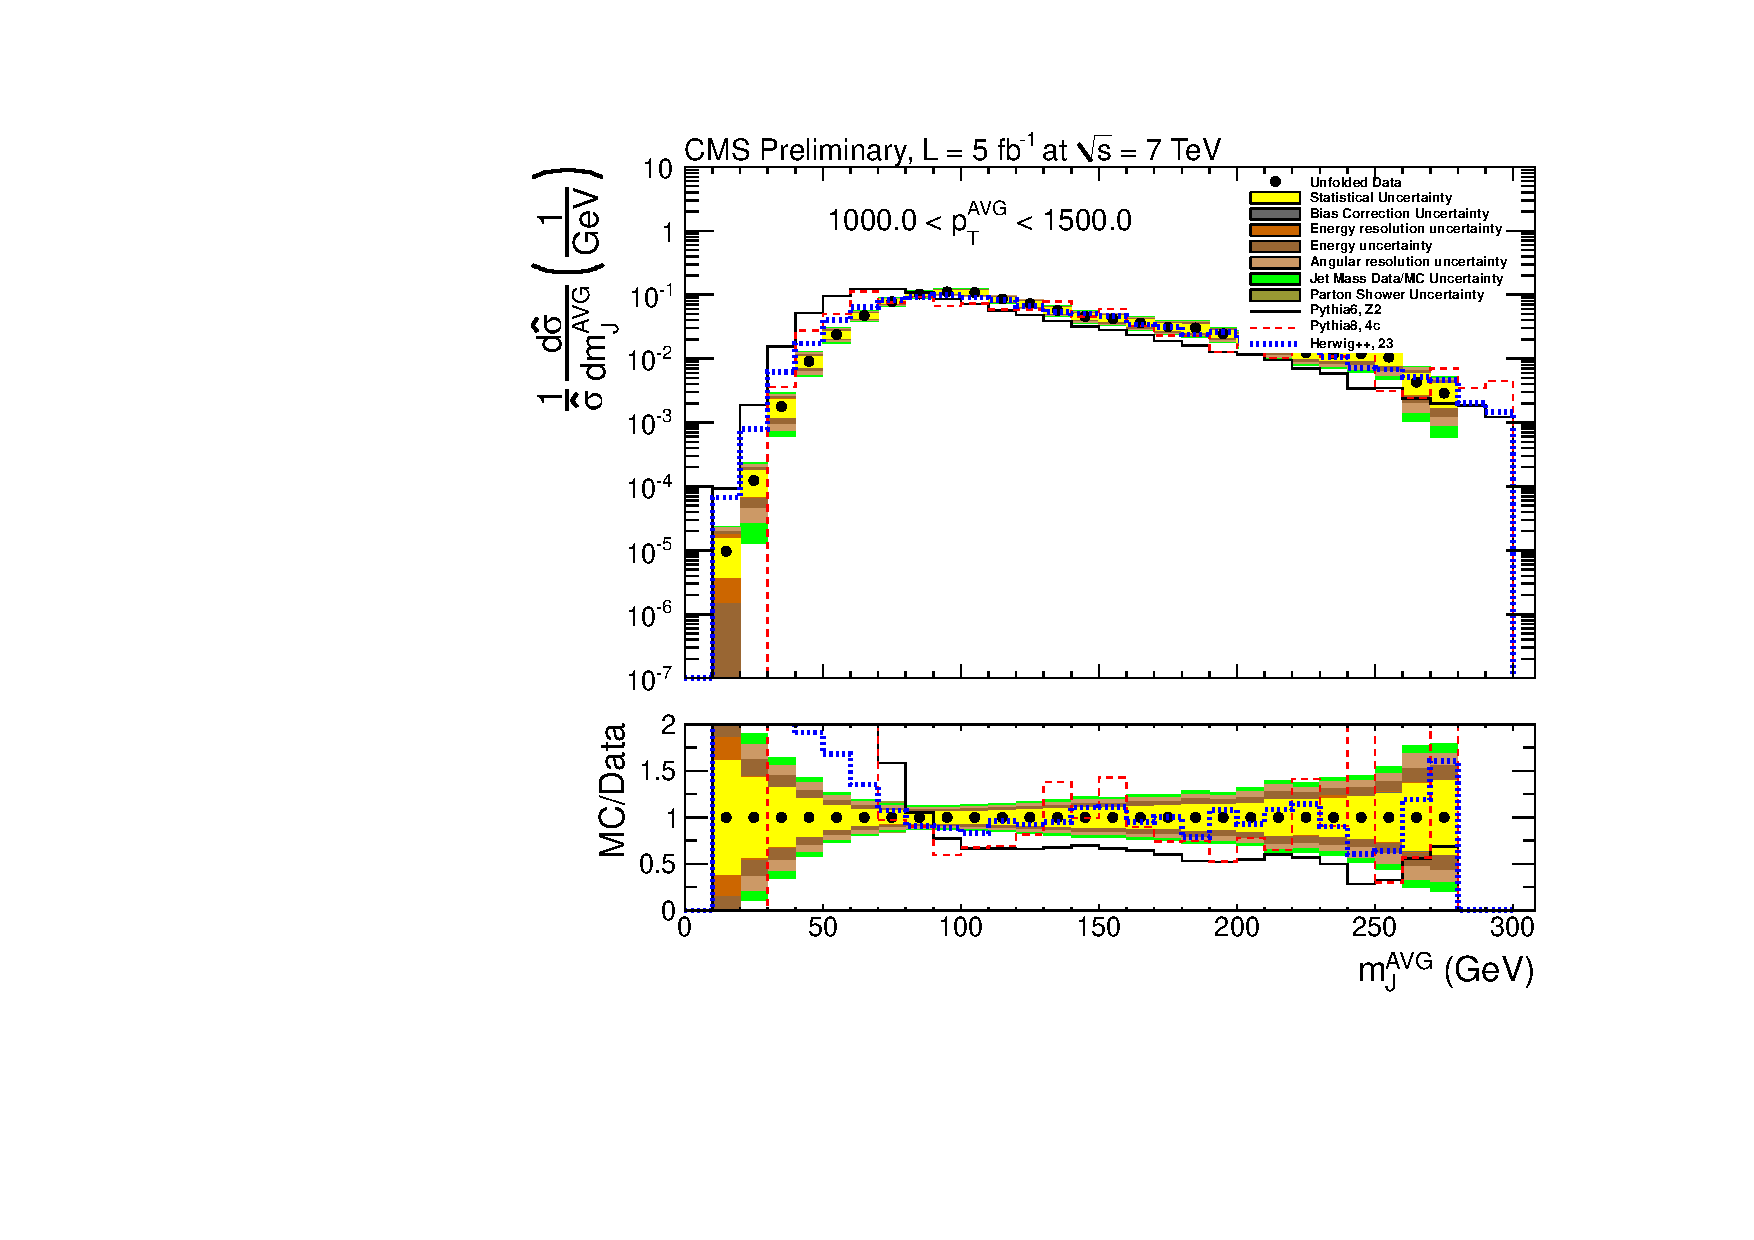
\includegraphics[width=0.95\textwidth]{figs/unfoldedMeasurementDijets_10_allsys}
\caption{Unfolded distributions of the jet mass for AK7 jets,
for $1000.0 < \pt^{AVG} < 1500.0$ \GeVc. The data are shown in black
points. 
The statistical uncertainty is shown in light yellow, the uncertainties due to the jet-energy resolution, jet-energy scale, and jet-angular resolution are shown in shades of brown, the uncertainty due to pile-up is shown in green, and the uncertainty due to the parton shower are shown in dark yellow.
The simulated distribution from \PYTHIA is shown in solid black, 
the from \PYTHIAEIGHT in dashed red, and from \HERWIG in dotted blue. 
The bottom frame shows the ratio of the true distribution from
the simulation divided by the unfolded distribution, along with
the uncertainties in the unfolded distribution. 
\label{figs:unfoldedMeasurementDijets_10_allsys}}
\end{figure}

\clearpage

\begin{figure}[htbp]
\centering
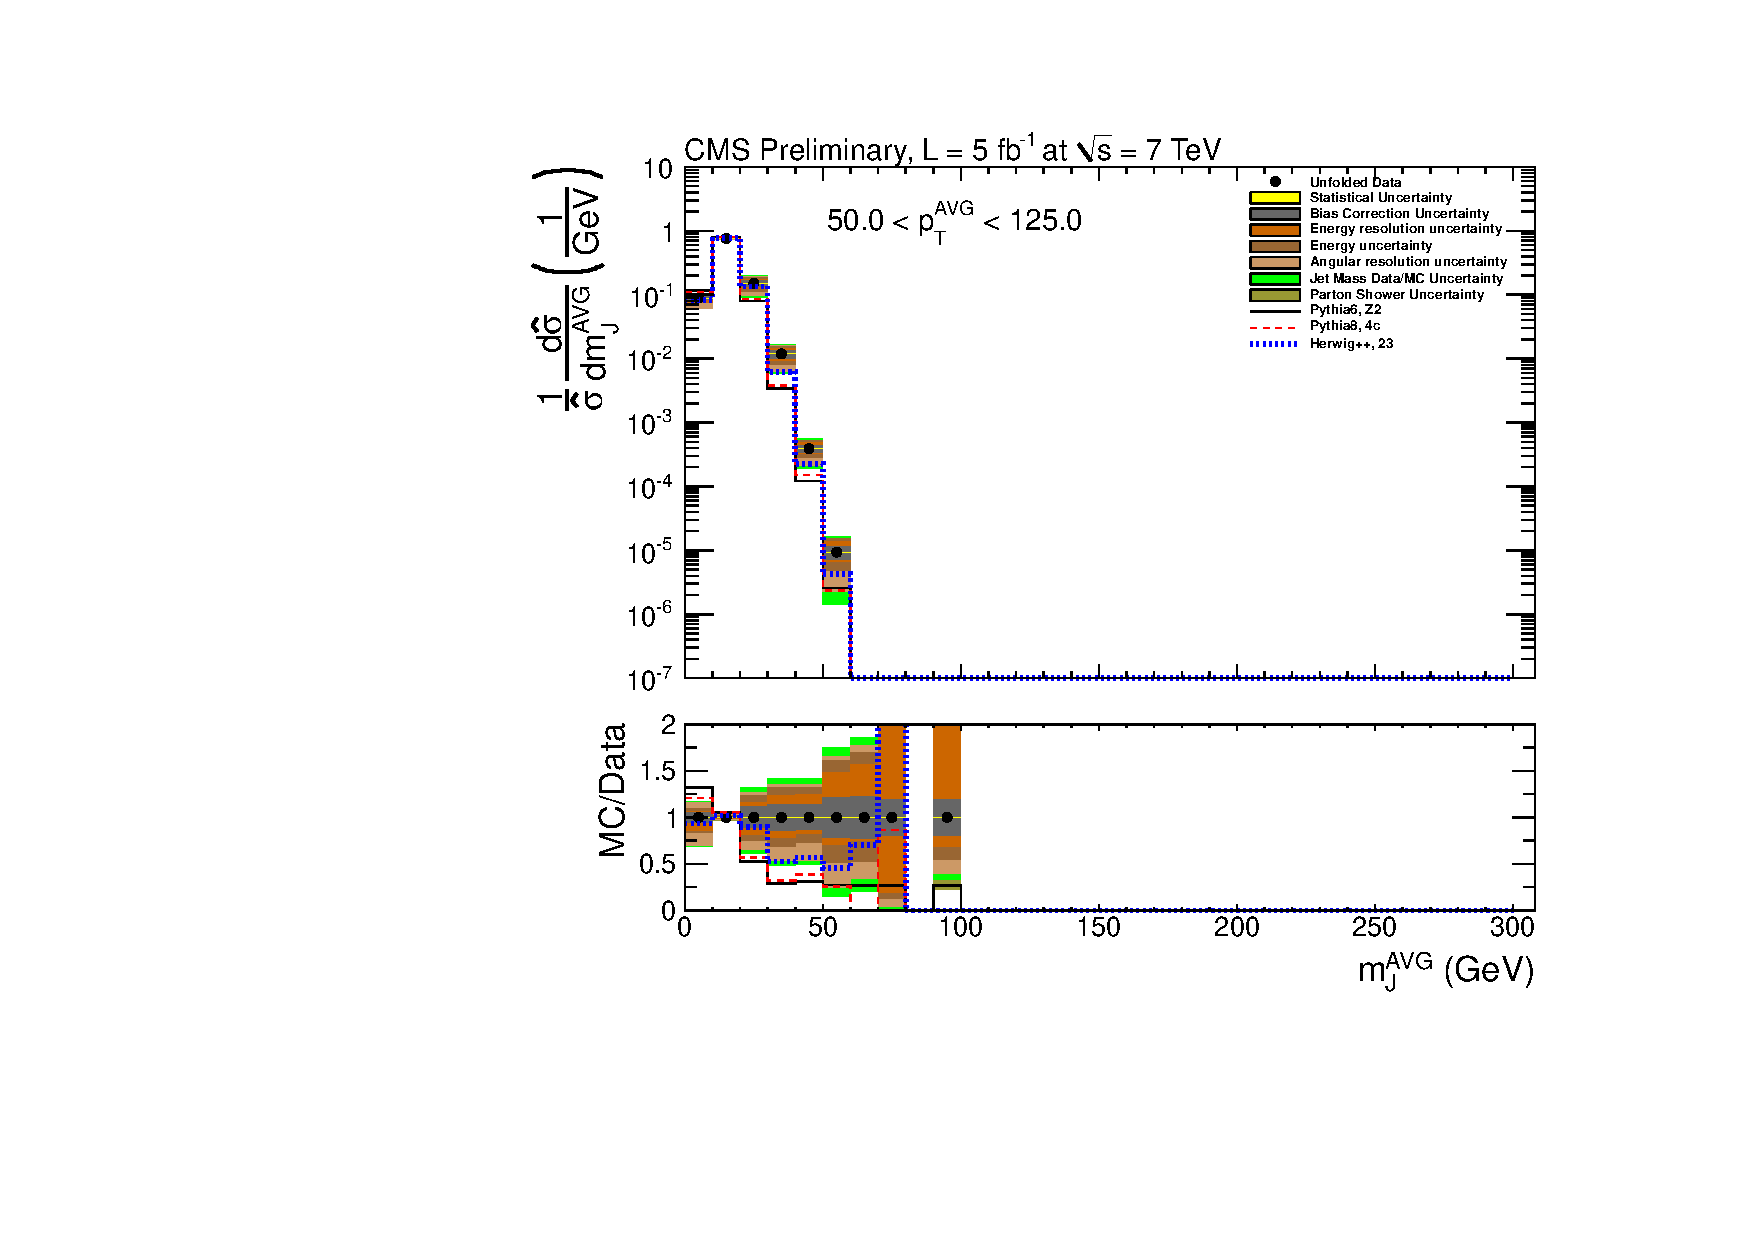
\includegraphics[width=0.95\textwidth]{figs/unfoldedMeasurementDijets_1_Filtered_allsys}
\caption{Unfolded distributions of the jet mass for AK7 Filtered jets,
for $50.0 < \pt^{AVG} < 125.0$ \GeVc. The data are shown in black
points. 
The statistical uncertainty is shown in light yellow, the uncertainties due to the jet-energy resolution, jet-energy scale, and jet-angular resolution are shown in shades of brown, the uncertainty due to pile-up is shown in green, and the uncertainty due to the parton shower are shown in dark yellow.
The simulated distribution from \PYTHIA is shown in solid black, 
the from \PYTHIAEIGHT in dashed red, and from \HERWIG in dotted blue. 
The bottom frame shows the ratio of the true distribution from
the simulation divided by the unfolded distribution, along with
the uncertainties in the unfolded distribution. 
\label{figs:unfoldedMeasurementDijets_1_Filtered_allsys}}
\end{figure}



\begin{figure}[htbp]
\centering
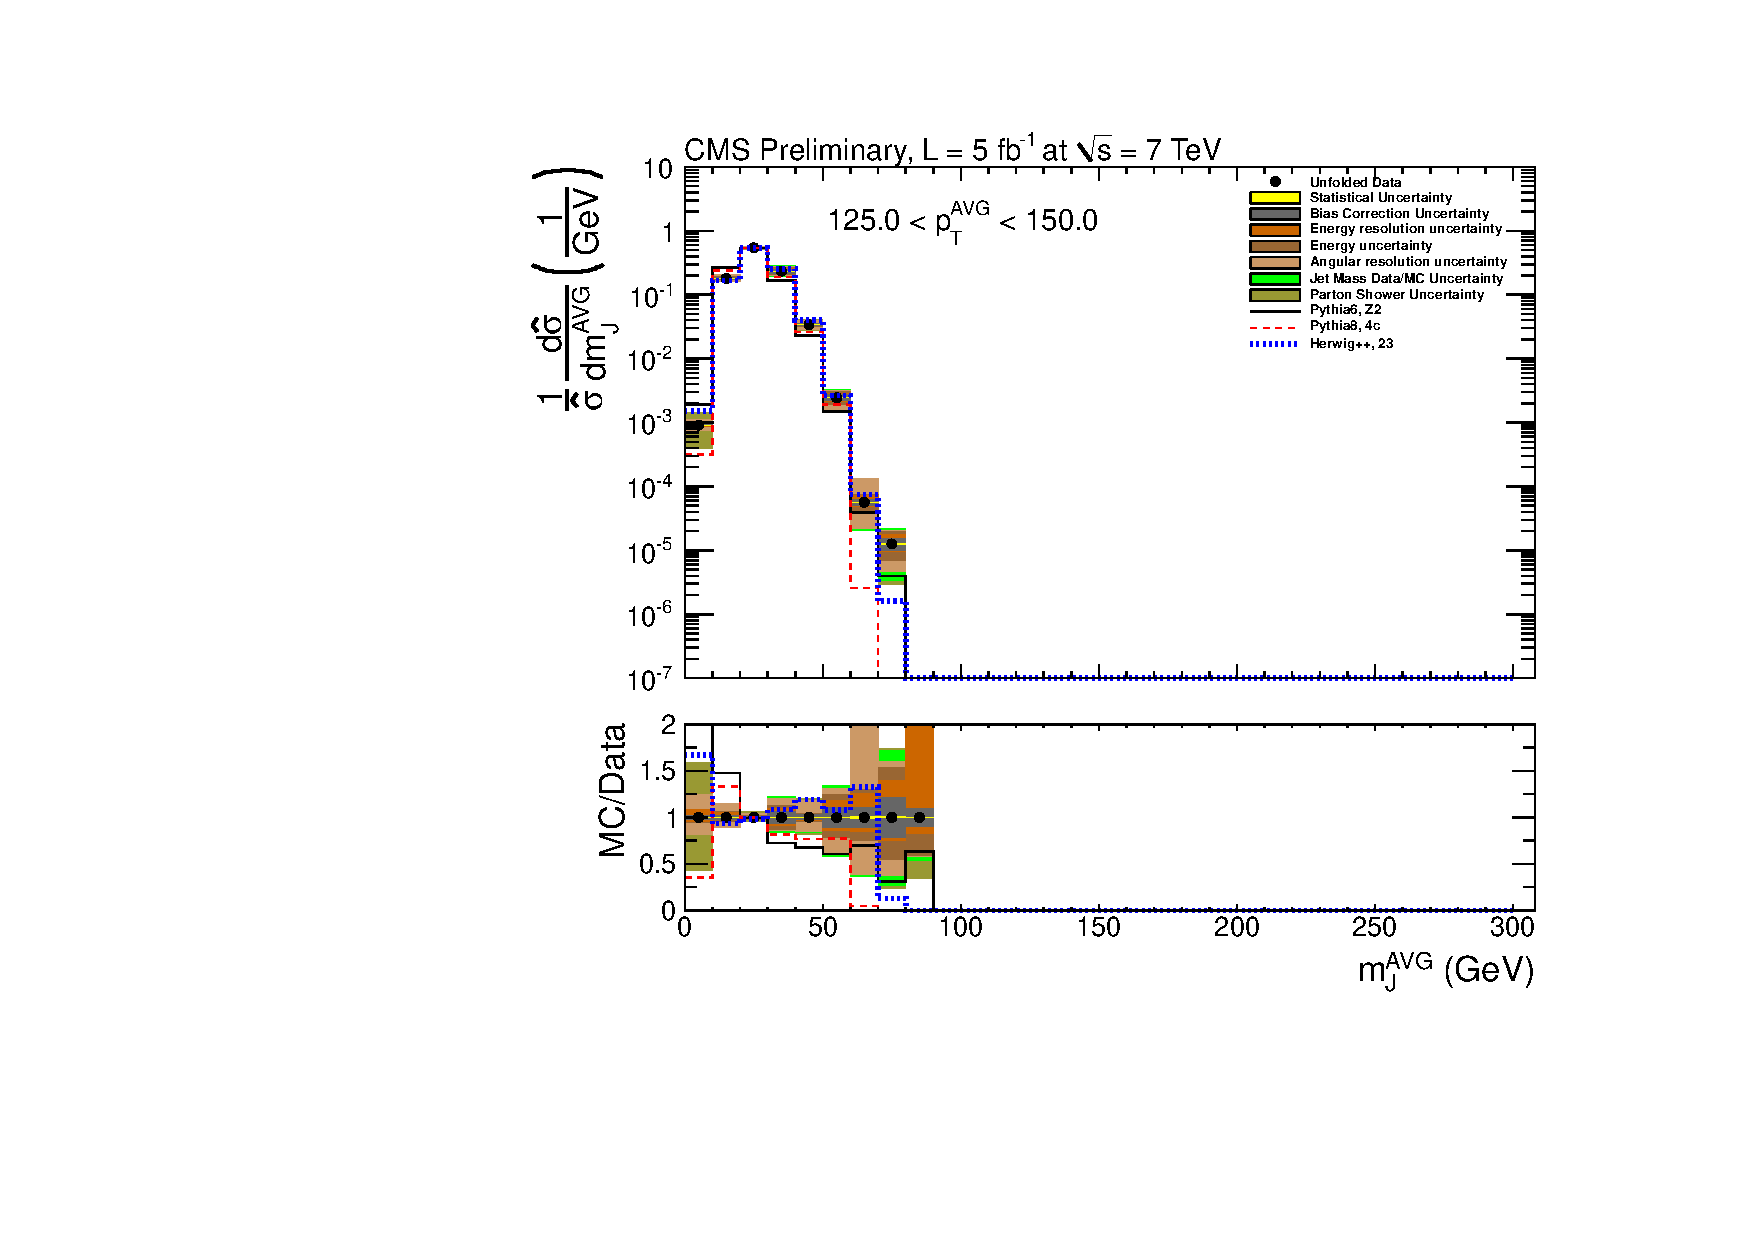
\includegraphics[width=0.95\textwidth]{figs/unfoldedMeasurementDijets_2_Filtered_allsys}
\caption{Unfolded distributions of the jet mass for AK7 Filtered jets,
for $125.0 < \pt^{AVG} < 150.0$ \GeVc. The data are shown in black
points. 
The statistical uncertainty is shown in light yellow, the uncertainties due to the jet-energy resolution, jet-energy scale, and jet-angular resolution are shown in shades of brown, the uncertainty due to pile-up is shown in green, and the uncertainty due to the parton shower are shown in dark yellow.
The simulated distribution from \PYTHIA is shown in solid black, 
the from \PYTHIAEIGHT in dashed red, and from \HERWIG in dotted blue. 
The bottom frame shows the ratio of the true distribution from
the simulation divided by the unfolded distribution, along with
the uncertainties in the unfolded distribution. 
\label{figs:unfoldedMeasurementDijets_2_Filtered_allsys}}
\end{figure}



\begin{figure}[htbp]
\centering
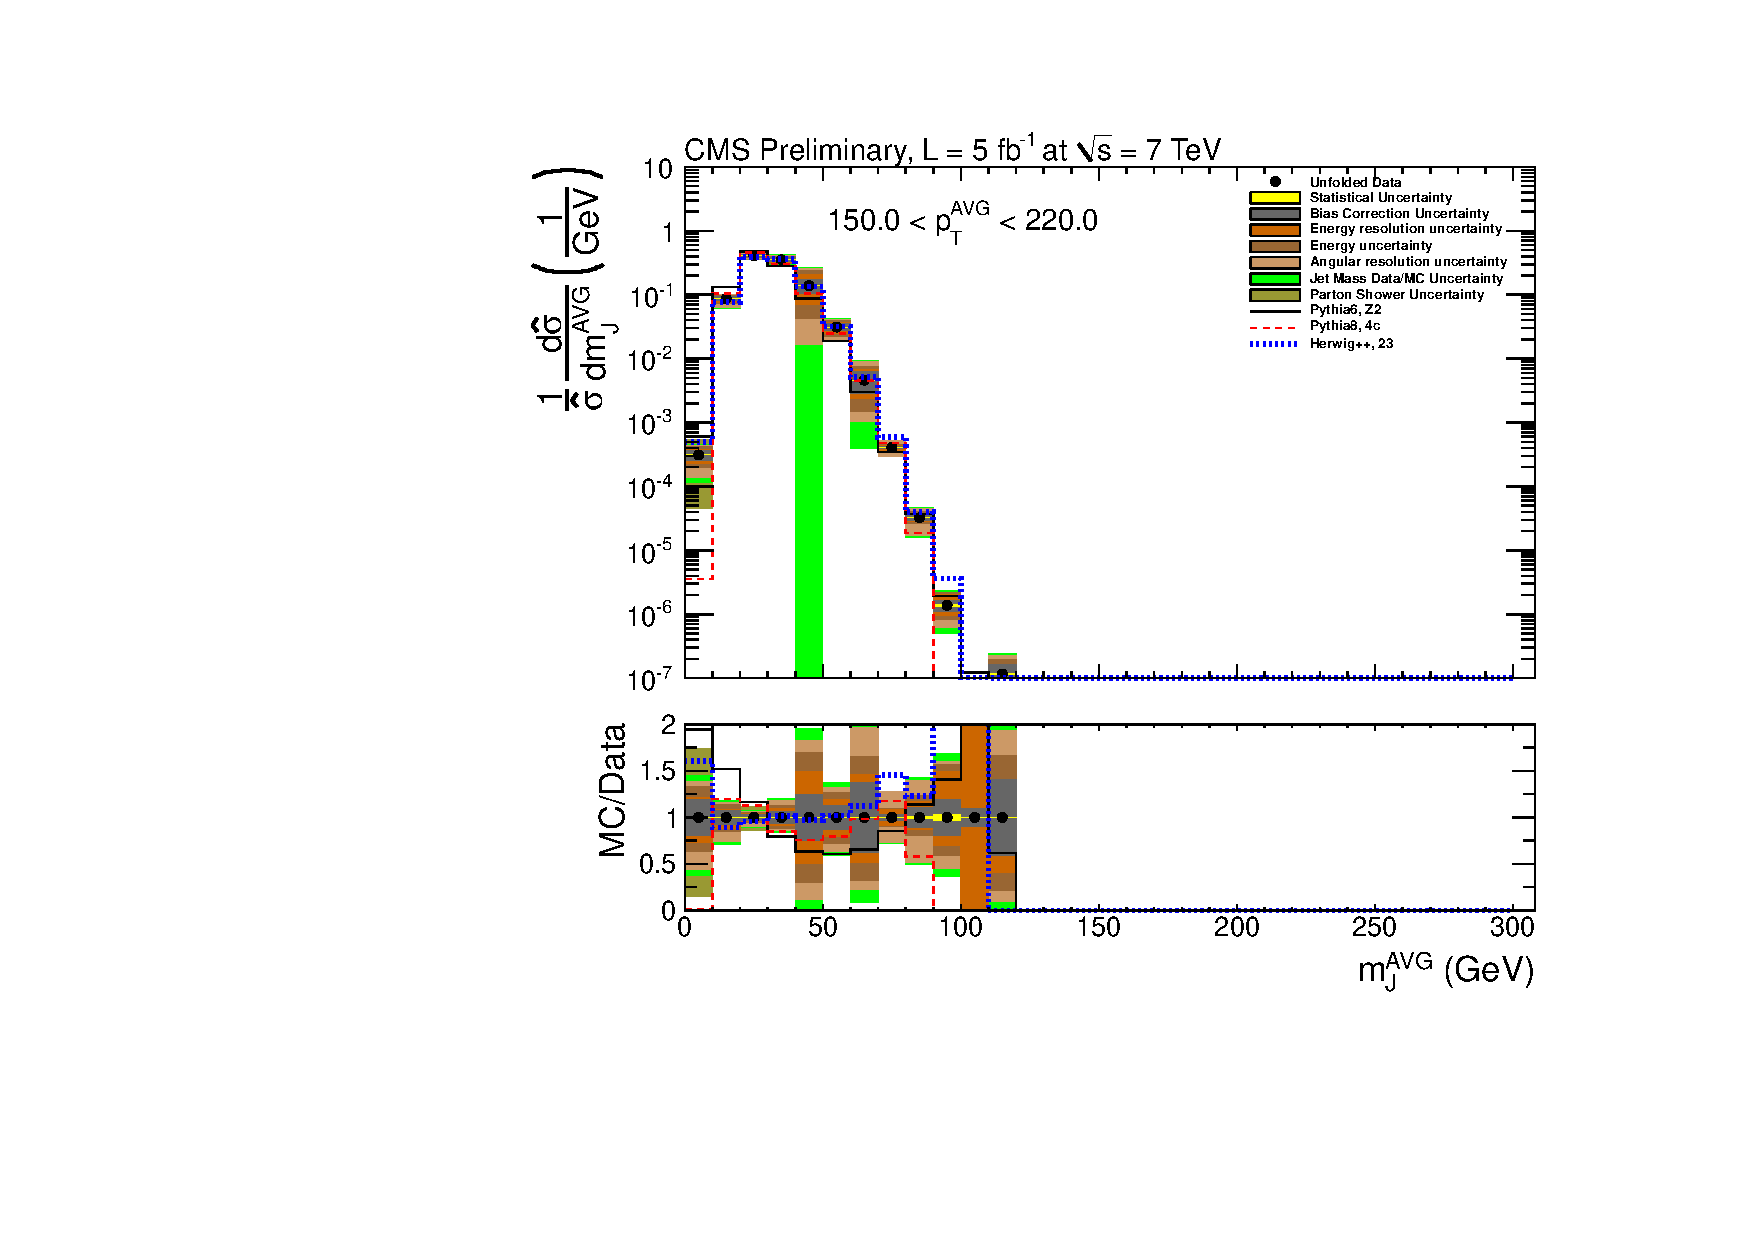
\includegraphics[width=0.95\textwidth]{figs/unfoldedMeasurementDijets_3_Filtered_allsys}
\caption{Unfolded distributions of the jet mass for AK7 Filtered jets,
for $150.0 < \pt^{AVG} < 220.0$ \GeVc. The data are shown in black
points. 
The statistical uncertainty is shown in light yellow, the uncertainties due to the jet-energy resolution, jet-energy scale, and jet-angular resolution are shown in shades of brown, the uncertainty due to pile-up is shown in green, and the uncertainty due to the parton shower are shown in dark yellow.
The simulated distribution from \PYTHIA is shown in solid black, 
the from \PYTHIAEIGHT in dashed red, and from \HERWIG in dotted blue. 
The bottom frame shows the ratio of the true distribution from
the simulation divided by the unfolded distribution, along with
the uncertainties in the unfolded distribution. 
\label{figs:unfoldedMeasurementDijets_3_Filtered_allsys}}
\end{figure}



\begin{figure}[htbp]
\centering
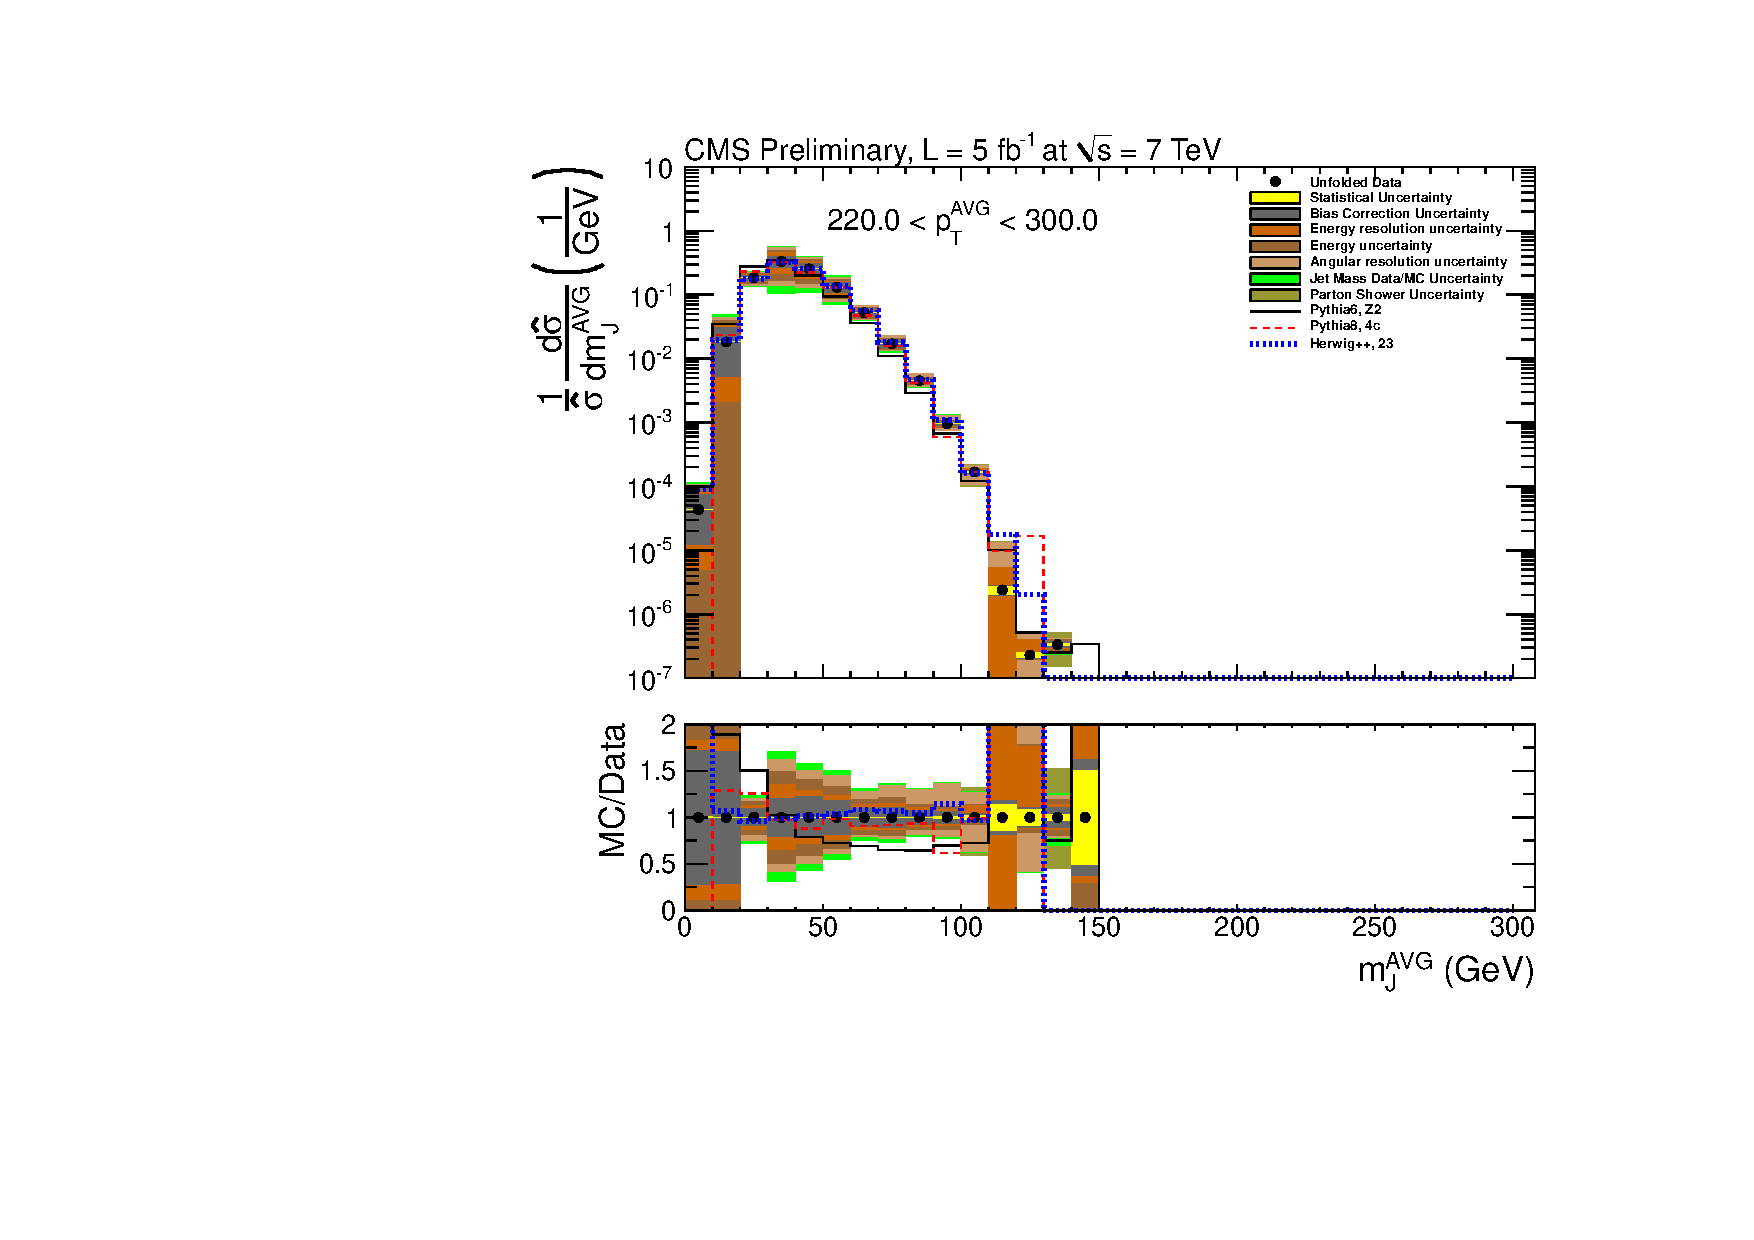
\includegraphics[width=0.95\textwidth]{figs/unfoldedMeasurementDijets_4_Filtered_allsys}
\caption{Unfolded distributions of the jet mass for AK7 Filtered jets,
for $220.0 < \pt^{AVG} < 300.0$ \GeVc. The data are shown in black
points. 
The statistical uncertainty is shown in light yellow, the uncertainties due to the jet-energy resolution, jet-energy scale, and jet-angular resolution are shown in shades of brown, the uncertainty due to pile-up is shown in green, and the uncertainty due to the parton shower are shown in dark yellow.
The simulated distribution from \PYTHIA is shown in solid black, 
the from \PYTHIAEIGHT in dashed red, and from \HERWIG in dotted blue. 
The bottom frame shows the ratio of the true distribution from
the simulation divided by the unfolded distribution, along with
the uncertainties in the unfolded distribution. 
\label{figs:unfoldedMeasurementDijets_4_Filtered_allsys}}
\end{figure}



\begin{figure}[htbp]
\centering
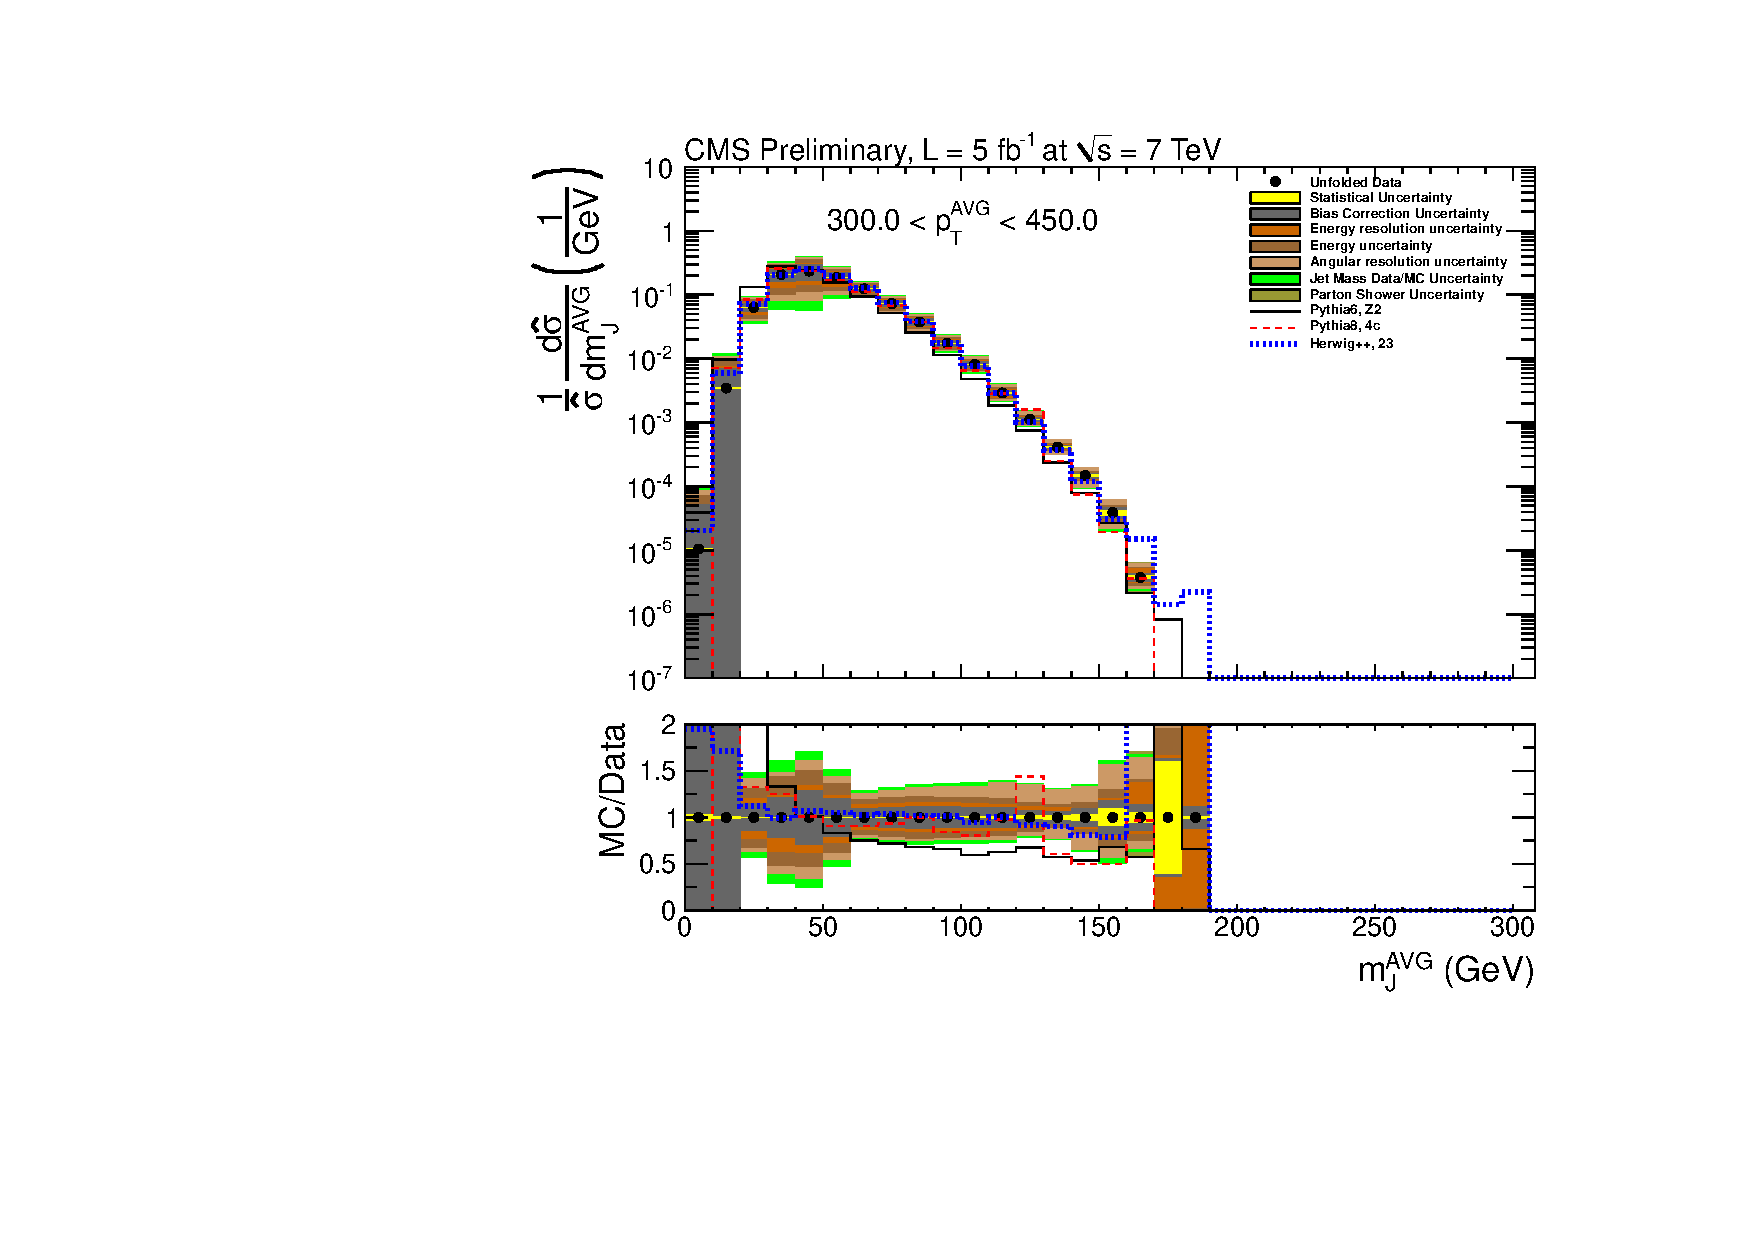
\includegraphics[width=0.95\textwidth]{figs/unfoldedMeasurementDijets_5_Filtered_allsys}
\caption{Unfolded distributions of the jet mass for AK7 Filtered jets,
for $300.0 < \pt^{AVG} < 450.0$ \GeVc. The data are shown in black
points. 
The statistical uncertainty is shown in light yellow, the uncertainties due to the jet-energy resolution, jet-energy scale, and jet-angular resolution are shown in shades of brown, the uncertainty due to pile-up is shown in green, and the uncertainty due to the parton shower are shown in dark yellow.
The simulated distribution from \PYTHIA is shown in solid black, 
the from \PYTHIAEIGHT in dashed red, and from \HERWIG in dotted blue. 
The bottom frame shows the ratio of the true distribution from
the simulation divided by the unfolded distribution, along with
the uncertainties in the unfolded distribution. 
\label{figs:unfoldedMeasurementDijets_5_Filtered_allsys}}
\end{figure}



\begin{figure}[htbp]
\centering
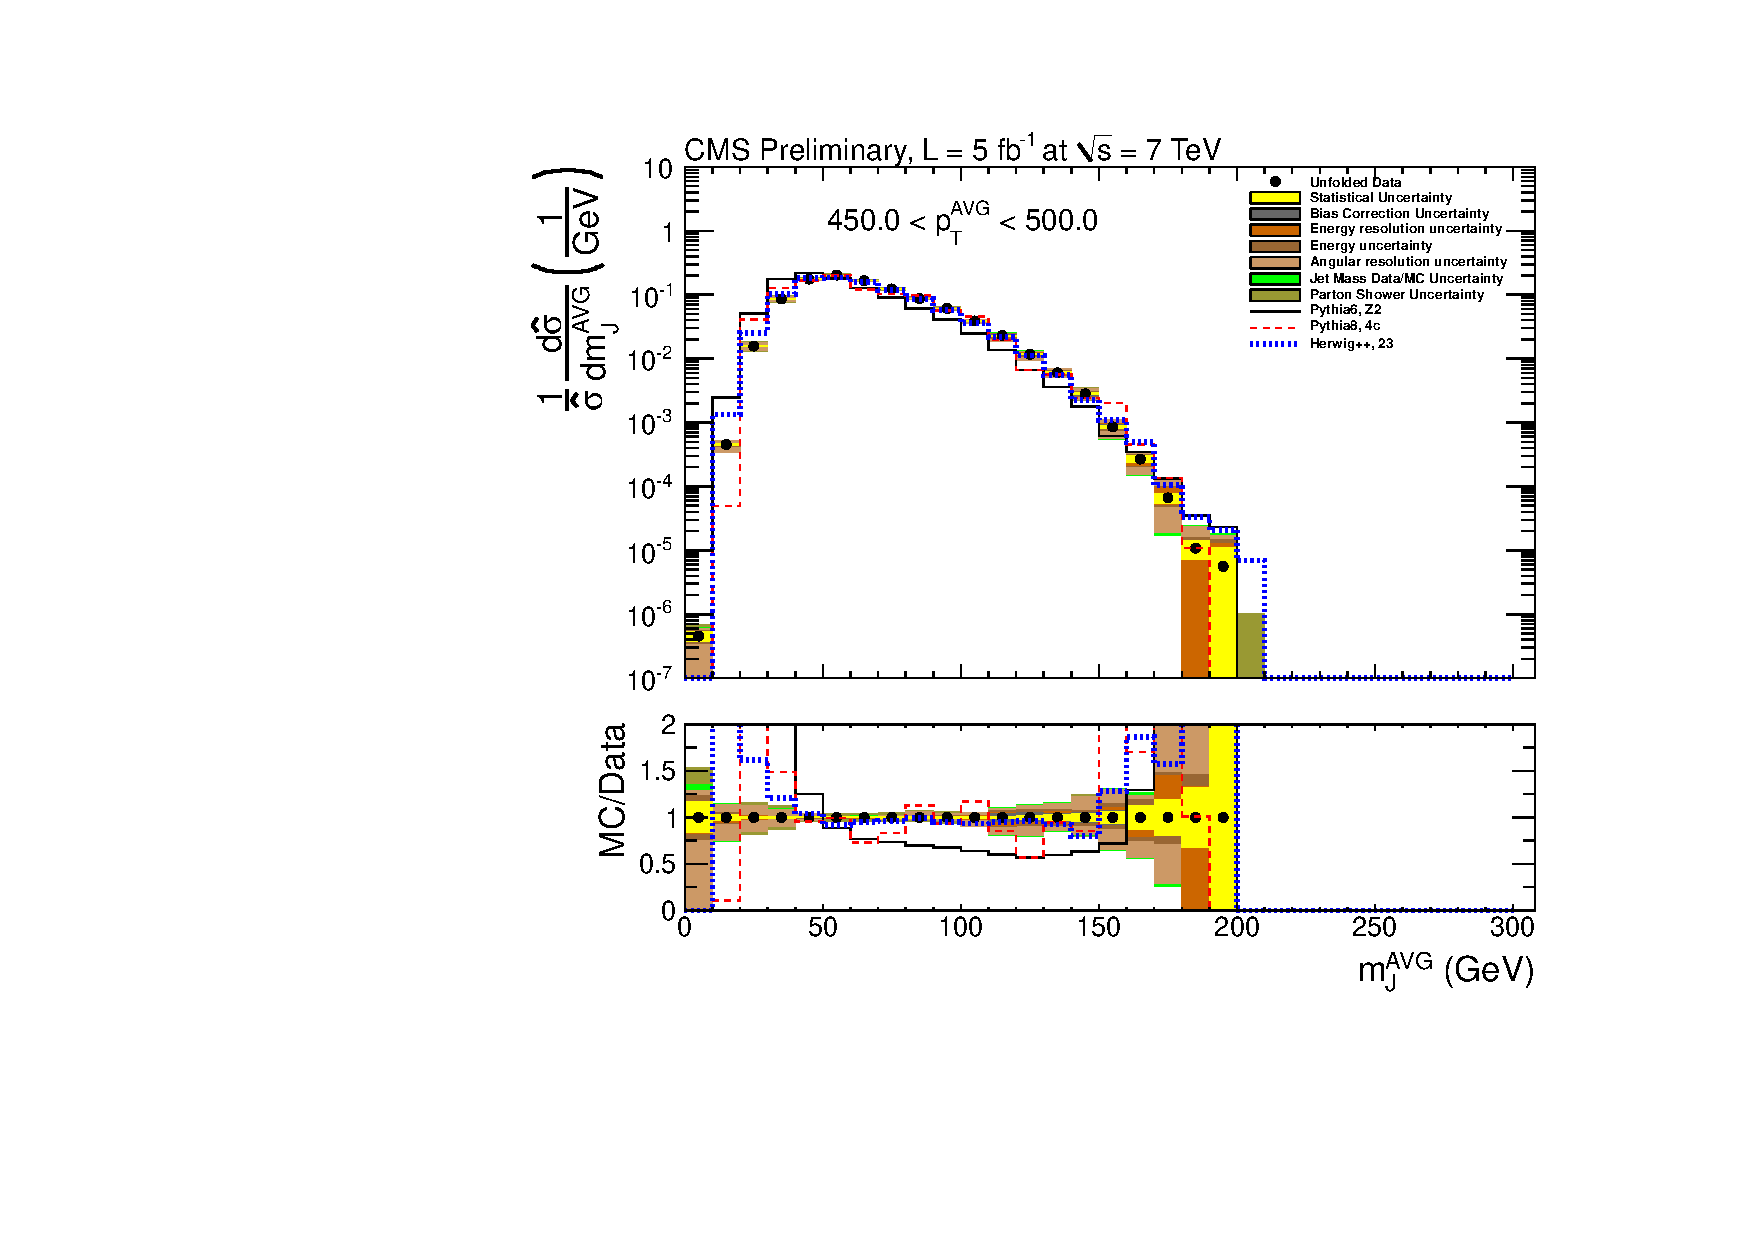
\includegraphics[width=0.95\textwidth]{figs/unfoldedMeasurementDijets_6_Filtered_allsys}
\caption{Unfolded distributions of the jet mass for AK7 Filtered jets,
for $450.0 < \pt^{AVG} < 500.0$ \GeVc. The data are shown in black
points. 
The statistical uncertainty is shown in light yellow, the uncertainties due to the jet-energy resolution, jet-energy scale, and jet-angular resolution are shown in shades of brown, the uncertainty due to pile-up is shown in green, and the uncertainty due to the parton shower are shown in dark yellow.
The simulated distribution from \PYTHIA is shown in solid black, 
the from \PYTHIAEIGHT in dashed red, and from \HERWIG in dotted blue. 
The bottom frame shows the ratio of the true distribution from
the simulation divided by the unfolded distribution, along with
the uncertainties in the unfolded distribution. 
\label{figs:unfoldedMeasurementDijets_6_Filtered_allsys}}
\end{figure}



\begin{figure}[htbp]
\centering
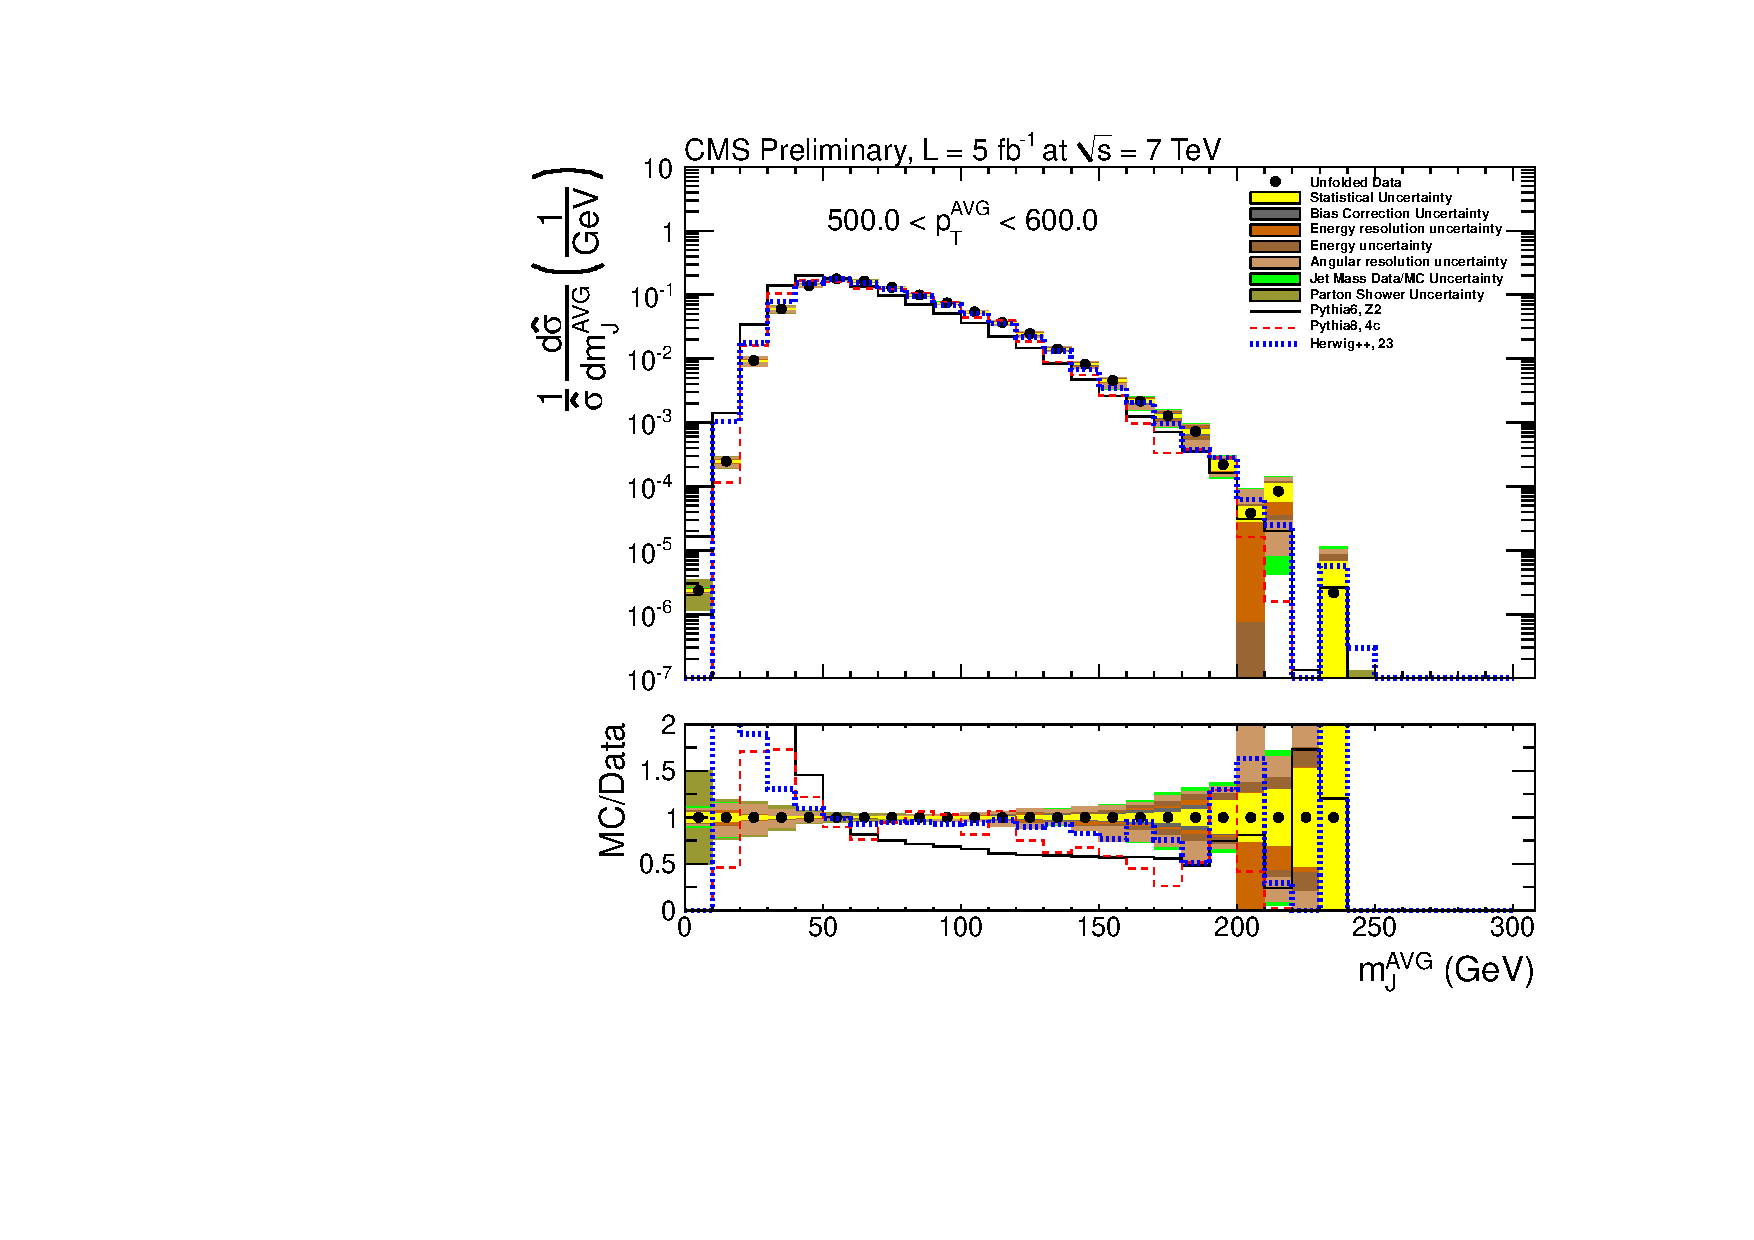
\includegraphics[width=0.95\textwidth]{figs/unfoldedMeasurementDijets_7_Filtered_allsys}
\caption{Unfolded distributions of the jet mass for AK7 Filtered jets,
for $500.0 < \pt^{AVG} < 600.0$ \GeVc. The data are shown in black
points. 
The statistical uncertainty is shown in light yellow, the uncertainties due to the jet-energy resolution, jet-energy scale, and jet-angular resolution are shown in shades of brown, the uncertainty due to pile-up is shown in green, and the uncertainty due to the parton shower are shown in dark yellow.
The simulated distribution from \PYTHIA is shown in solid black, 
the from \PYTHIAEIGHT in dashed red, and from \HERWIG in dotted blue. 
The bottom frame shows the ratio of the true distribution from
the simulation divided by the unfolded distribution, along with
the uncertainties in the unfolded distribution. 
\label{figs:unfoldedMeasurementDijets_7_Filtered_allsys}}
\end{figure}



\begin{figure}[htbp]
\centering
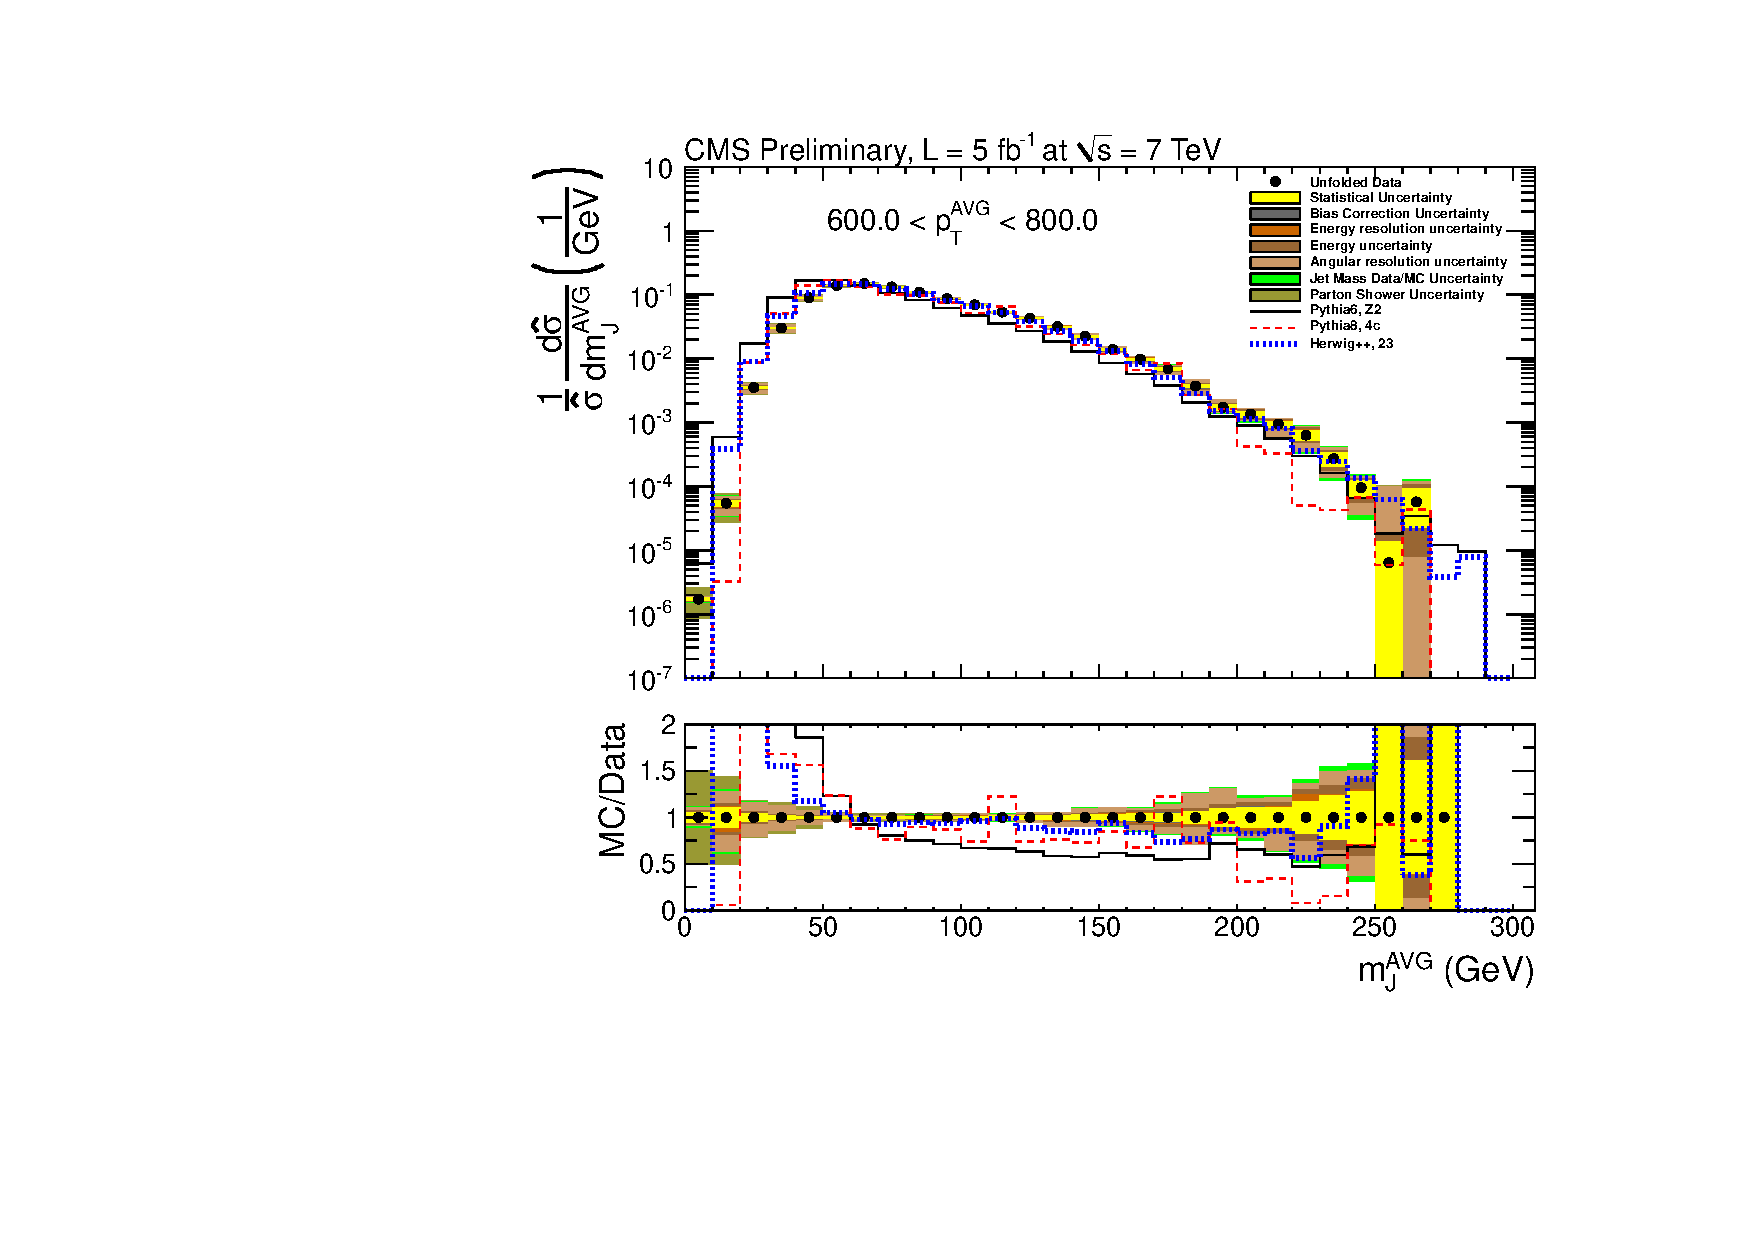
\includegraphics[width=0.95\textwidth]{figs/unfoldedMeasurementDijets_8_Filtered_allsys}
\caption{Unfolded distributions of the jet mass for AK7 Filtered jets,
for $600.0 < \pt^{AVG} < 800.0$ \GeVc. The data are shown in black
points. 
The statistical uncertainty is shown in light yellow, the uncertainties due to the jet-energy resolution, jet-energy scale, and jet-angular resolution are shown in shades of brown, the uncertainty due to pile-up is shown in green, and the uncertainty due to the parton shower are shown in dark yellow.
The simulated distribution from \PYTHIA is shown in solid black, 
the from \PYTHIAEIGHT in dashed red, and from \HERWIG in dotted blue. 
The bottom frame shows the ratio of the true distribution from
the simulation divided by the unfolded distribution, along with
the uncertainties in the unfolded distribution. 
\label{figs:unfoldedMeasurementDijets_8_Filtered_allsys}}
\end{figure}



\begin{figure}[htbp]
\centering
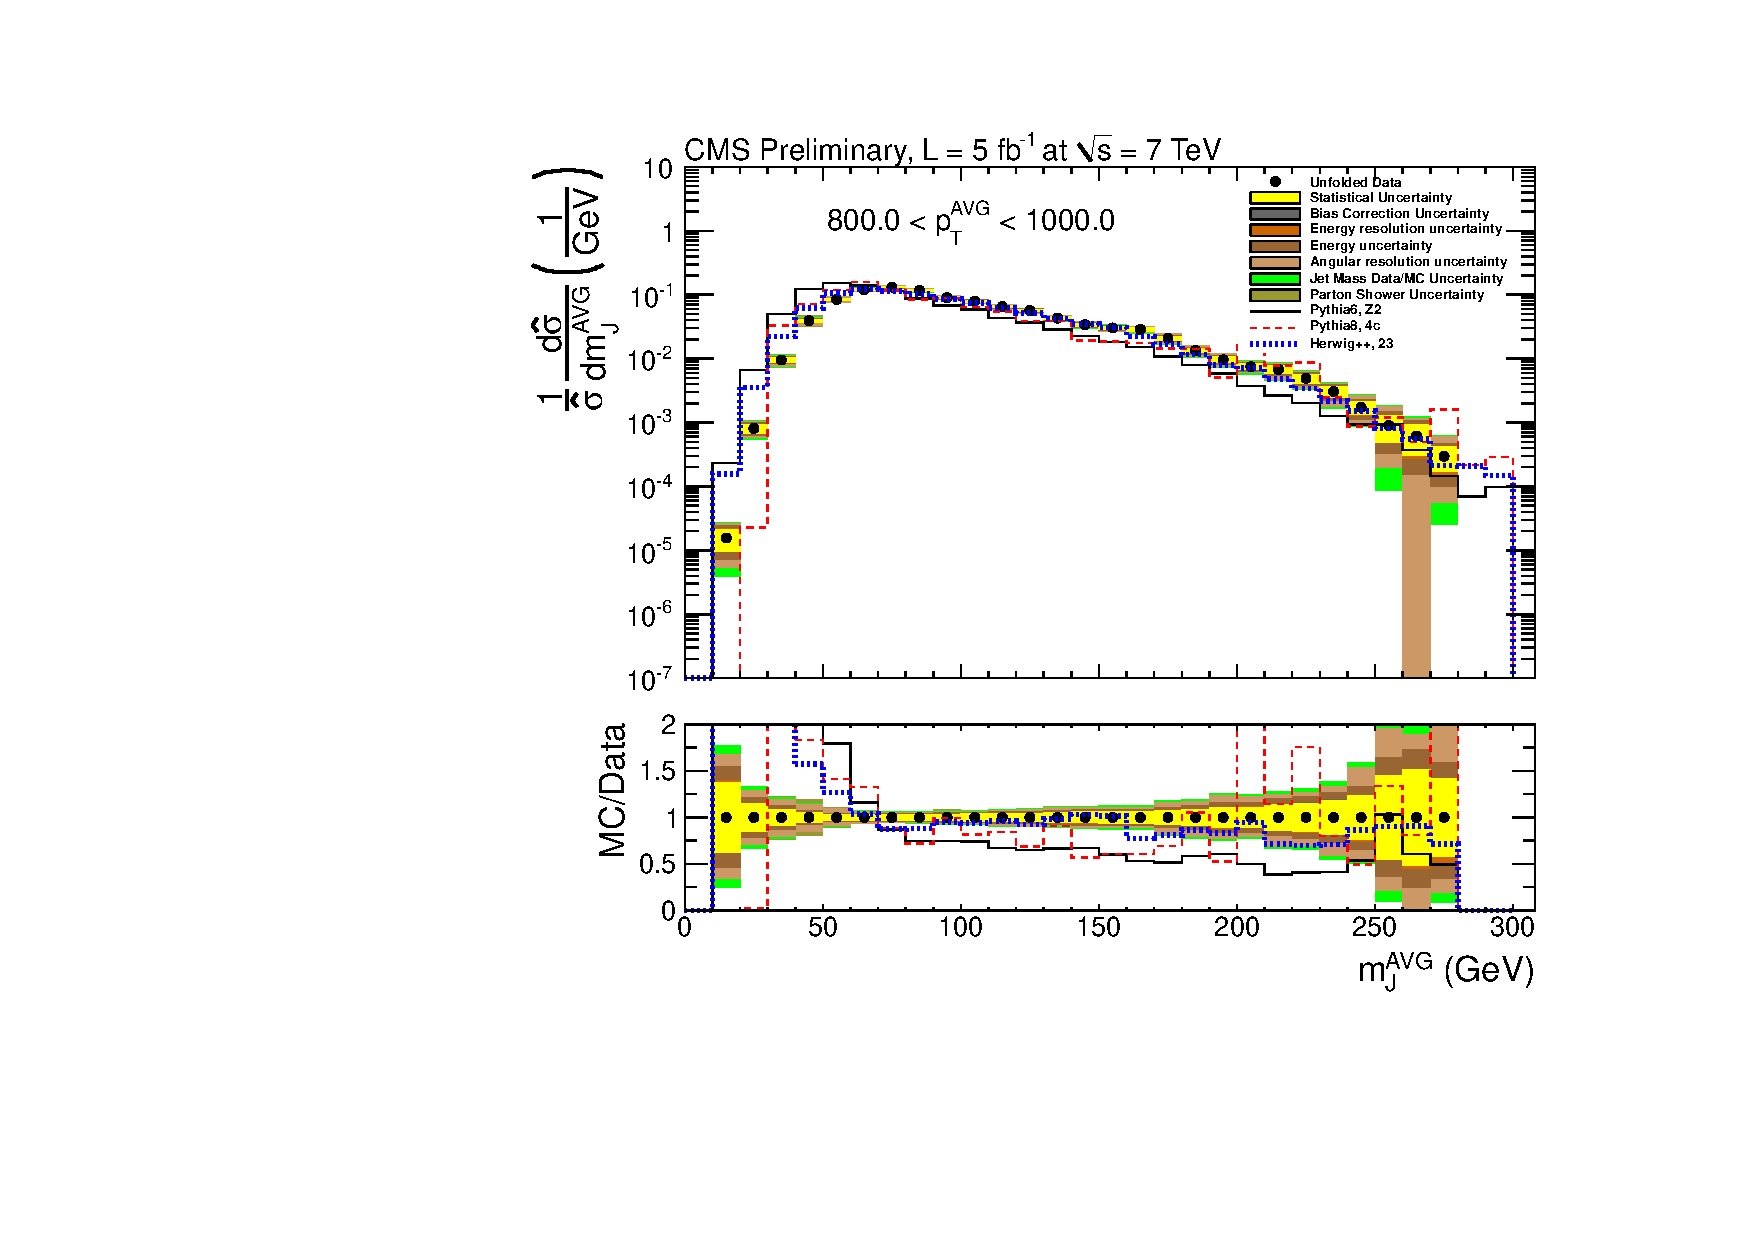
\includegraphics[width=0.95\textwidth]{figs/unfoldedMeasurementDijets_9_Filtered_allsys}
\caption{Unfolded distributions of the jet mass for AK7 Filtered jets,
for $800.0 < \pt^{AVG} < 1000.0$ \GeVc. The data are shown in black
points. 
The statistical uncertainty is shown in light yellow, the uncertainties due to the jet-energy resolution, jet-energy scale, and jet-angular resolution are shown in shades of brown, the uncertainty due to pile-up is shown in green, and the uncertainty due to the parton shower are shown in dark yellow.
The simulated distribution from \PYTHIA is shown in solid black, 
the from \PYTHIAEIGHT in dashed red, and from \HERWIG in dotted blue. 
The bottom frame shows the ratio of the true distribution from
the simulation divided by the unfolded distribution, along with
the uncertainties in the unfolded distribution. 
\label{figs:unfoldedMeasurementDijets_9_Filtered_allsys}}
\end{figure}



\begin{figure}[htbp]
\centering
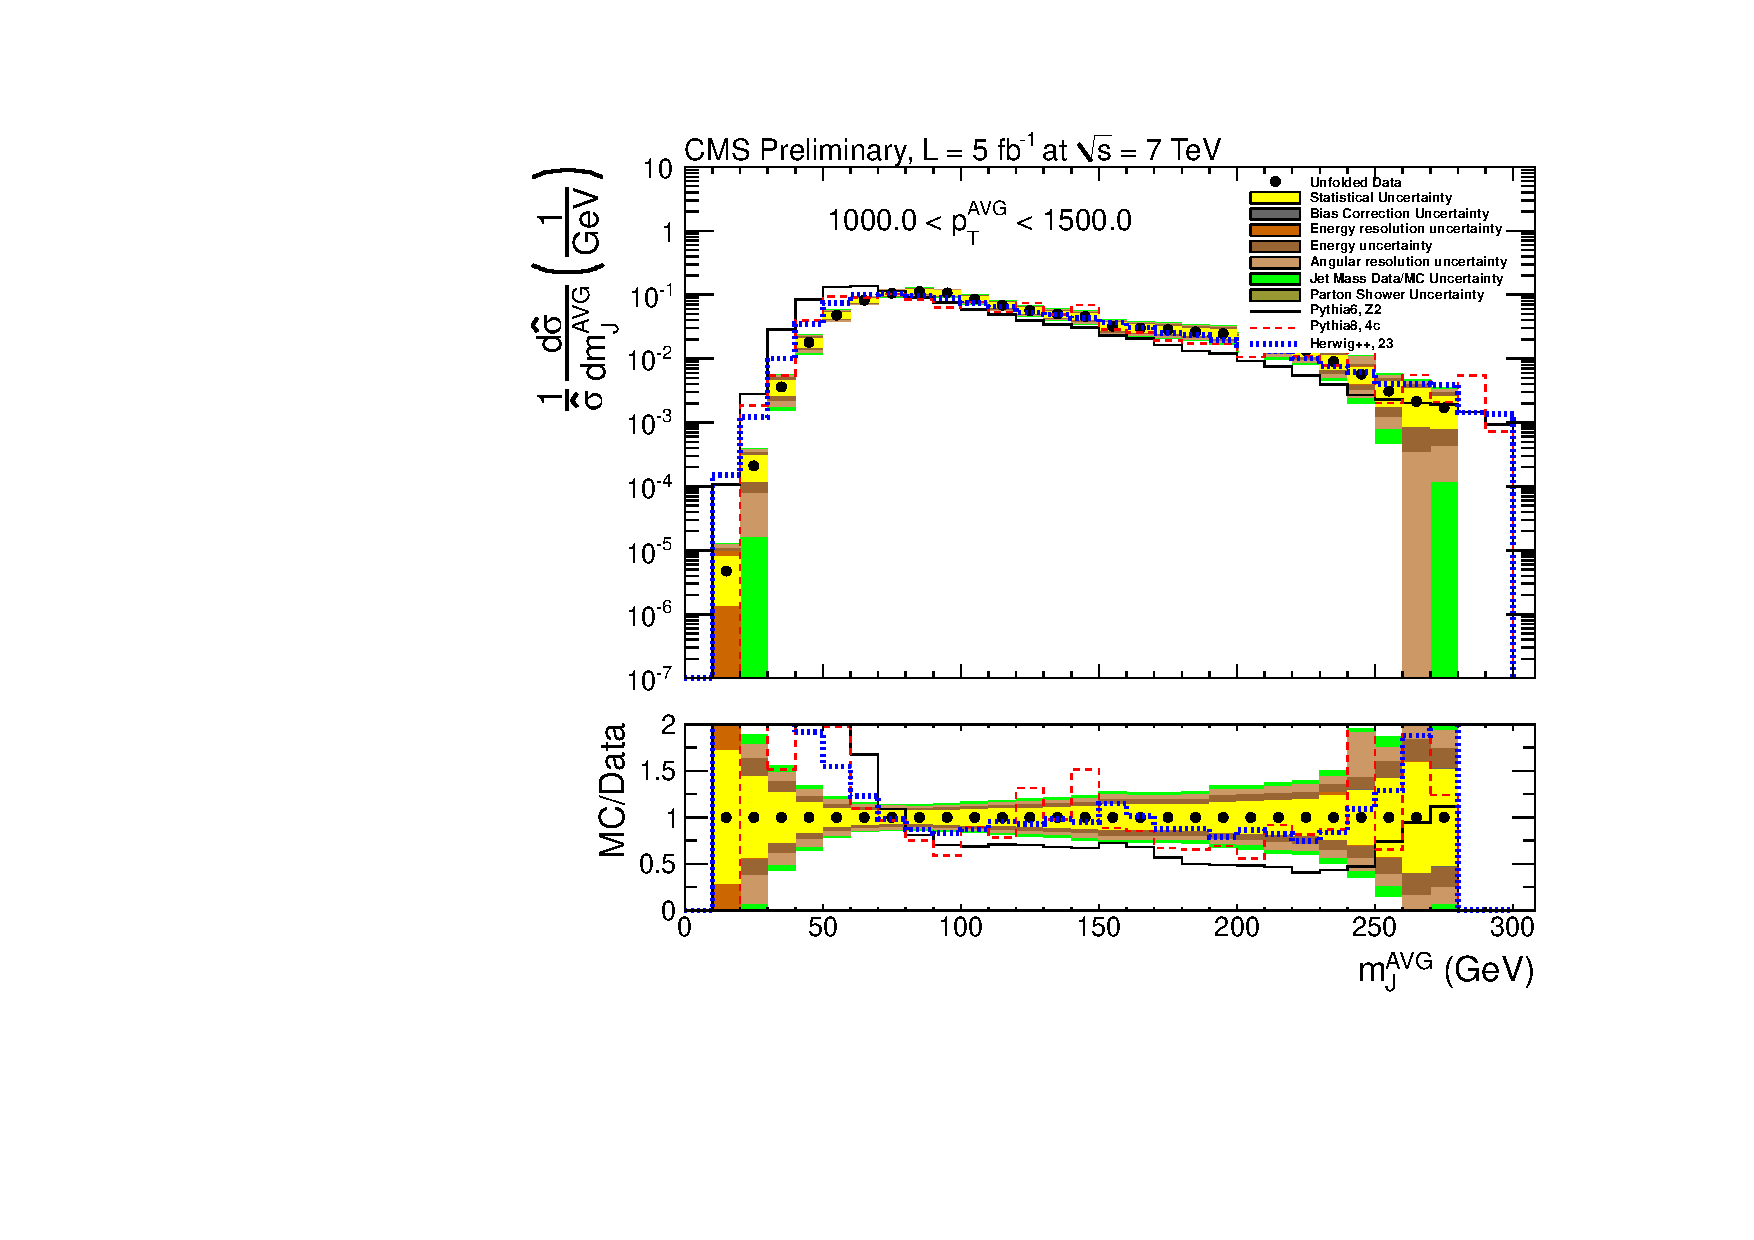
\includegraphics[width=0.95\textwidth]{figs/unfoldedMeasurementDijets_10_Filtered_allsys}
\caption{Unfolded distributions of the jet mass for AK7 Filtered jets,
for $1000.0 < \pt^{AVG} < 1500.0$ \GeVc. The data are shown in black
points. 
The statistical uncertainty is shown in light yellow, the uncertainties due to the jet-energy resolution, jet-energy scale, and jet-angular resolution are shown in shades of brown, the uncertainty due to pile-up is shown in green, and the uncertainty due to the parton shower are shown in dark yellow.
The simulated distribution from \PYTHIA is shown in solid black, 
the from \PYTHIAEIGHT in dashed red, and from \HERWIG in dotted blue. 
The bottom frame shows the ratio of the true distribution from
the simulation divided by the unfolded distribution, along with
the uncertainties in the unfolded distribution. 
\label{figs:unfoldedMeasurementDijets_10_Filtered_allsys}}
\end{figure}

\clearpage

\begin{figure}[htbp]
\centering
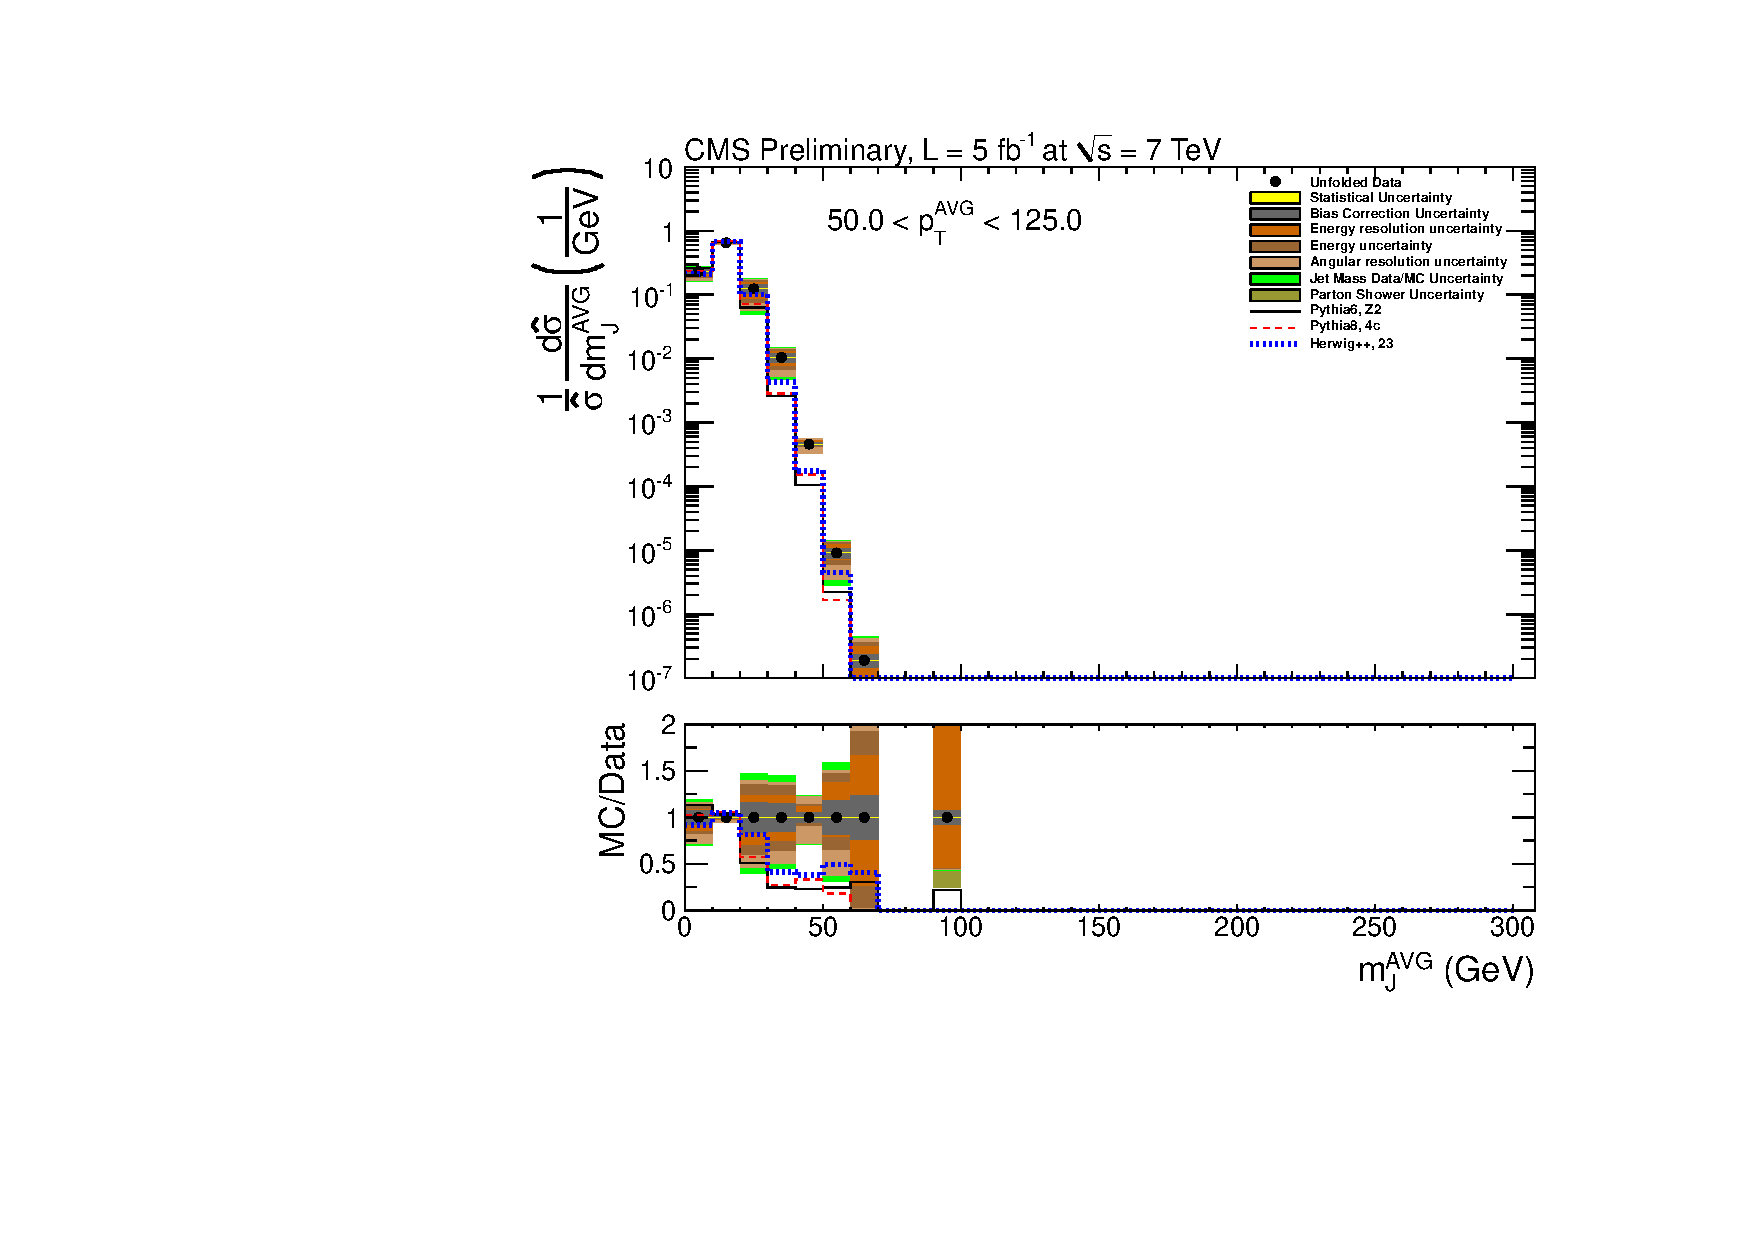
\includegraphics[width=0.95\textwidth]{figs/unfoldedMeasurementDijets_1_Trimmed_allsys}
\caption{Unfolded distributions of the jet mass for AK7 Trimmed jets,
for $50.0 < \pt^{AVG} < 125.0$ \GeVc. The data are shown in black
points. 
The statistical uncertainty is shown in light yellow, the uncertainties due to the jet-energy resolution, jet-energy scale, and jet-angular resolution are shown in shades of brown, the uncertainty due to pile-up is shown in green, and the uncertainty due to the parton shower are shown in dark yellow.
The simulated distribution from \PYTHIA is shown in solid black, 
the from \PYTHIAEIGHT in dashed red, and from \HERWIG in dotted blue. 
The bottom frame shows the ratio of the true distribution from
the simulation divided by the unfolded distribution, along with
the uncertainties in the unfolded distribution. 
\label{figs:unfoldedMeasurementDijets_1_Trimmed_allsys}}
\end{figure}



\begin{figure}[htbp]
\centering
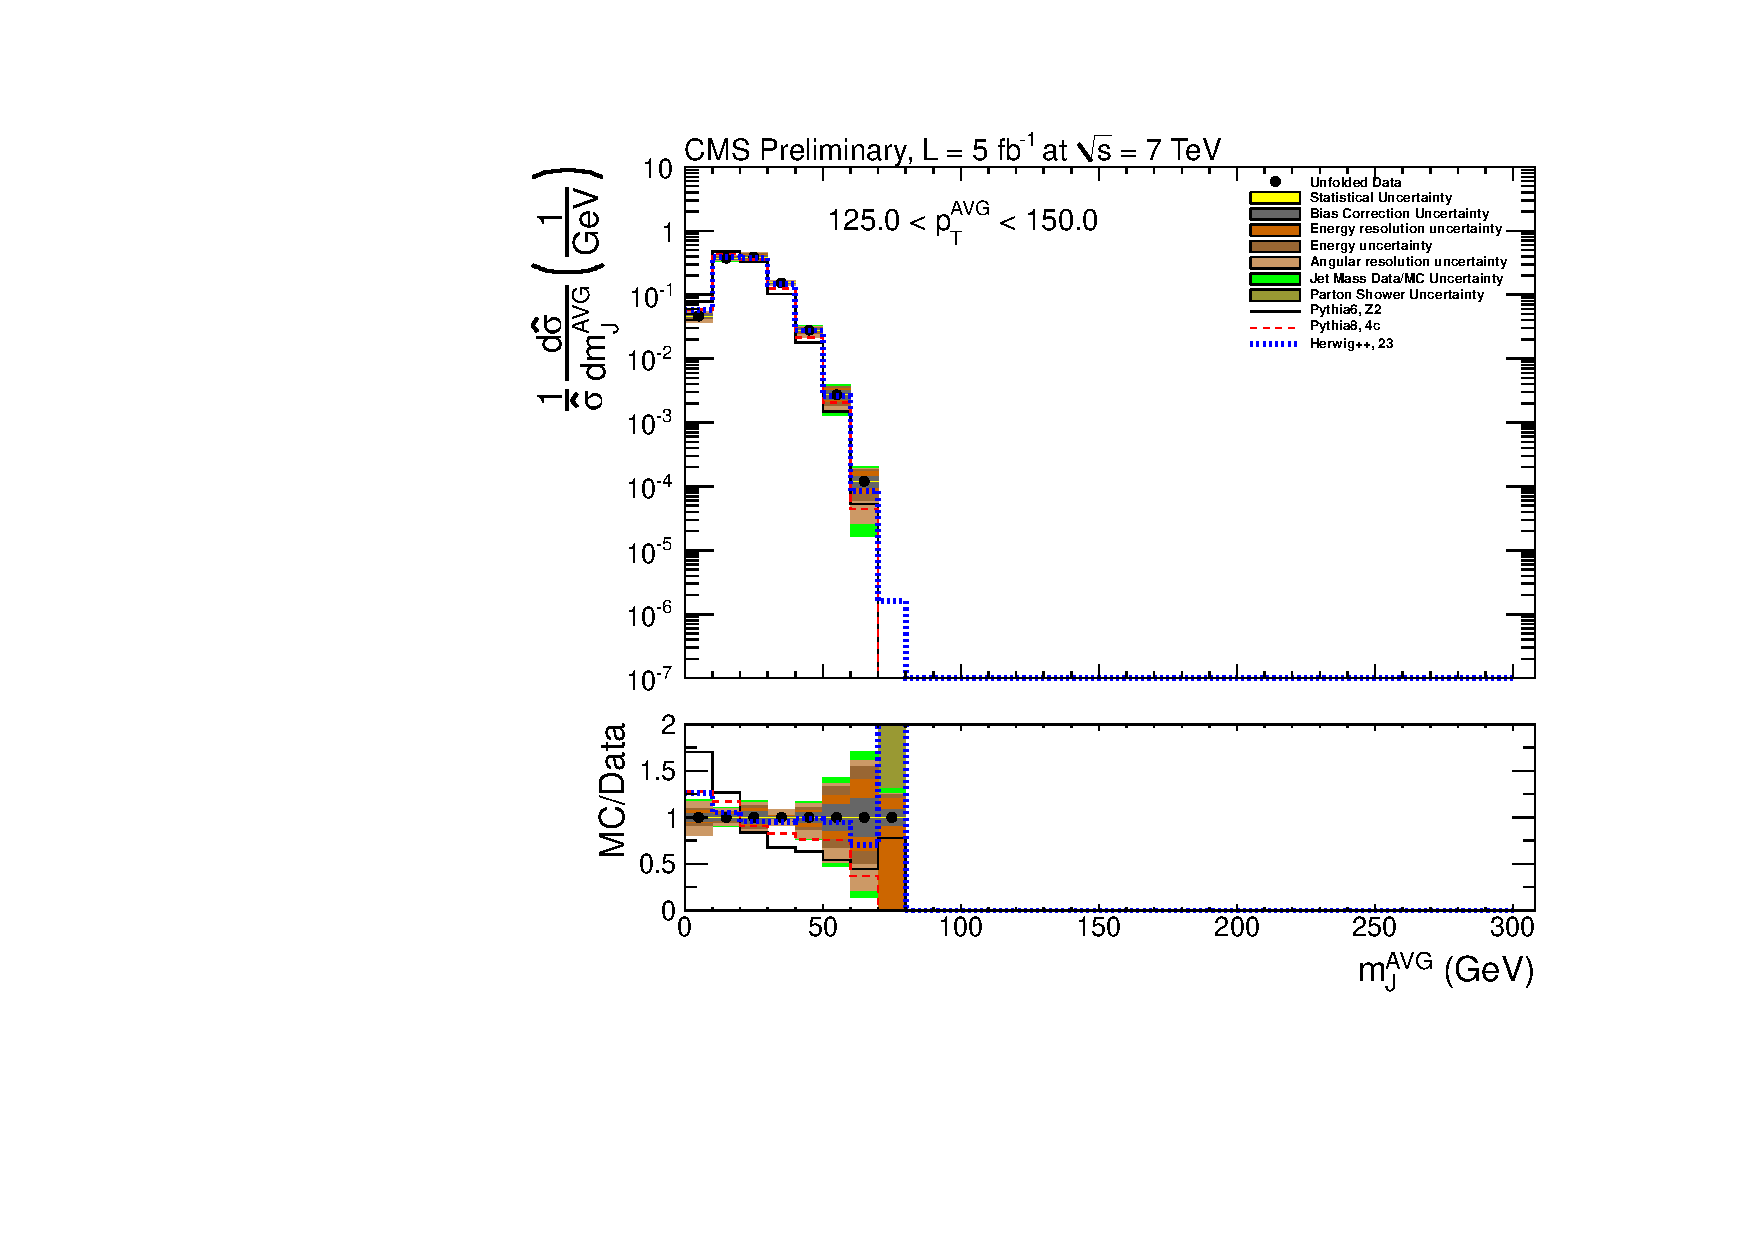
\includegraphics[width=0.95\textwidth]{figs/unfoldedMeasurementDijets_2_Trimmed_allsys}
\caption{Unfolded distributions of the jet mass for AK7 Trimmed jets,
for $125.0 < \pt^{AVG} < 150.0$ \GeVc. The data are shown in black
points. 
The statistical uncertainty is shown in light yellow, the uncertainties due to the jet-energy resolution, jet-energy scale, and jet-angular resolution are shown in shades of brown, the uncertainty due to pile-up is shown in green, and the uncertainty due to the parton shower are shown in dark yellow.
The simulated distribution from \PYTHIA is shown in solid black, 
the from \PYTHIAEIGHT in dashed red, and from \HERWIG in dotted blue. 
The bottom frame shows the ratio of the true distribution from
the simulation divided by the unfolded distribution, along with
the uncertainties in the unfolded distribution. 
\label{figs:unfoldedMeasurementDijets_2_Trimmed_allsys}}
\end{figure}



\begin{figure}[htbp]
\centering
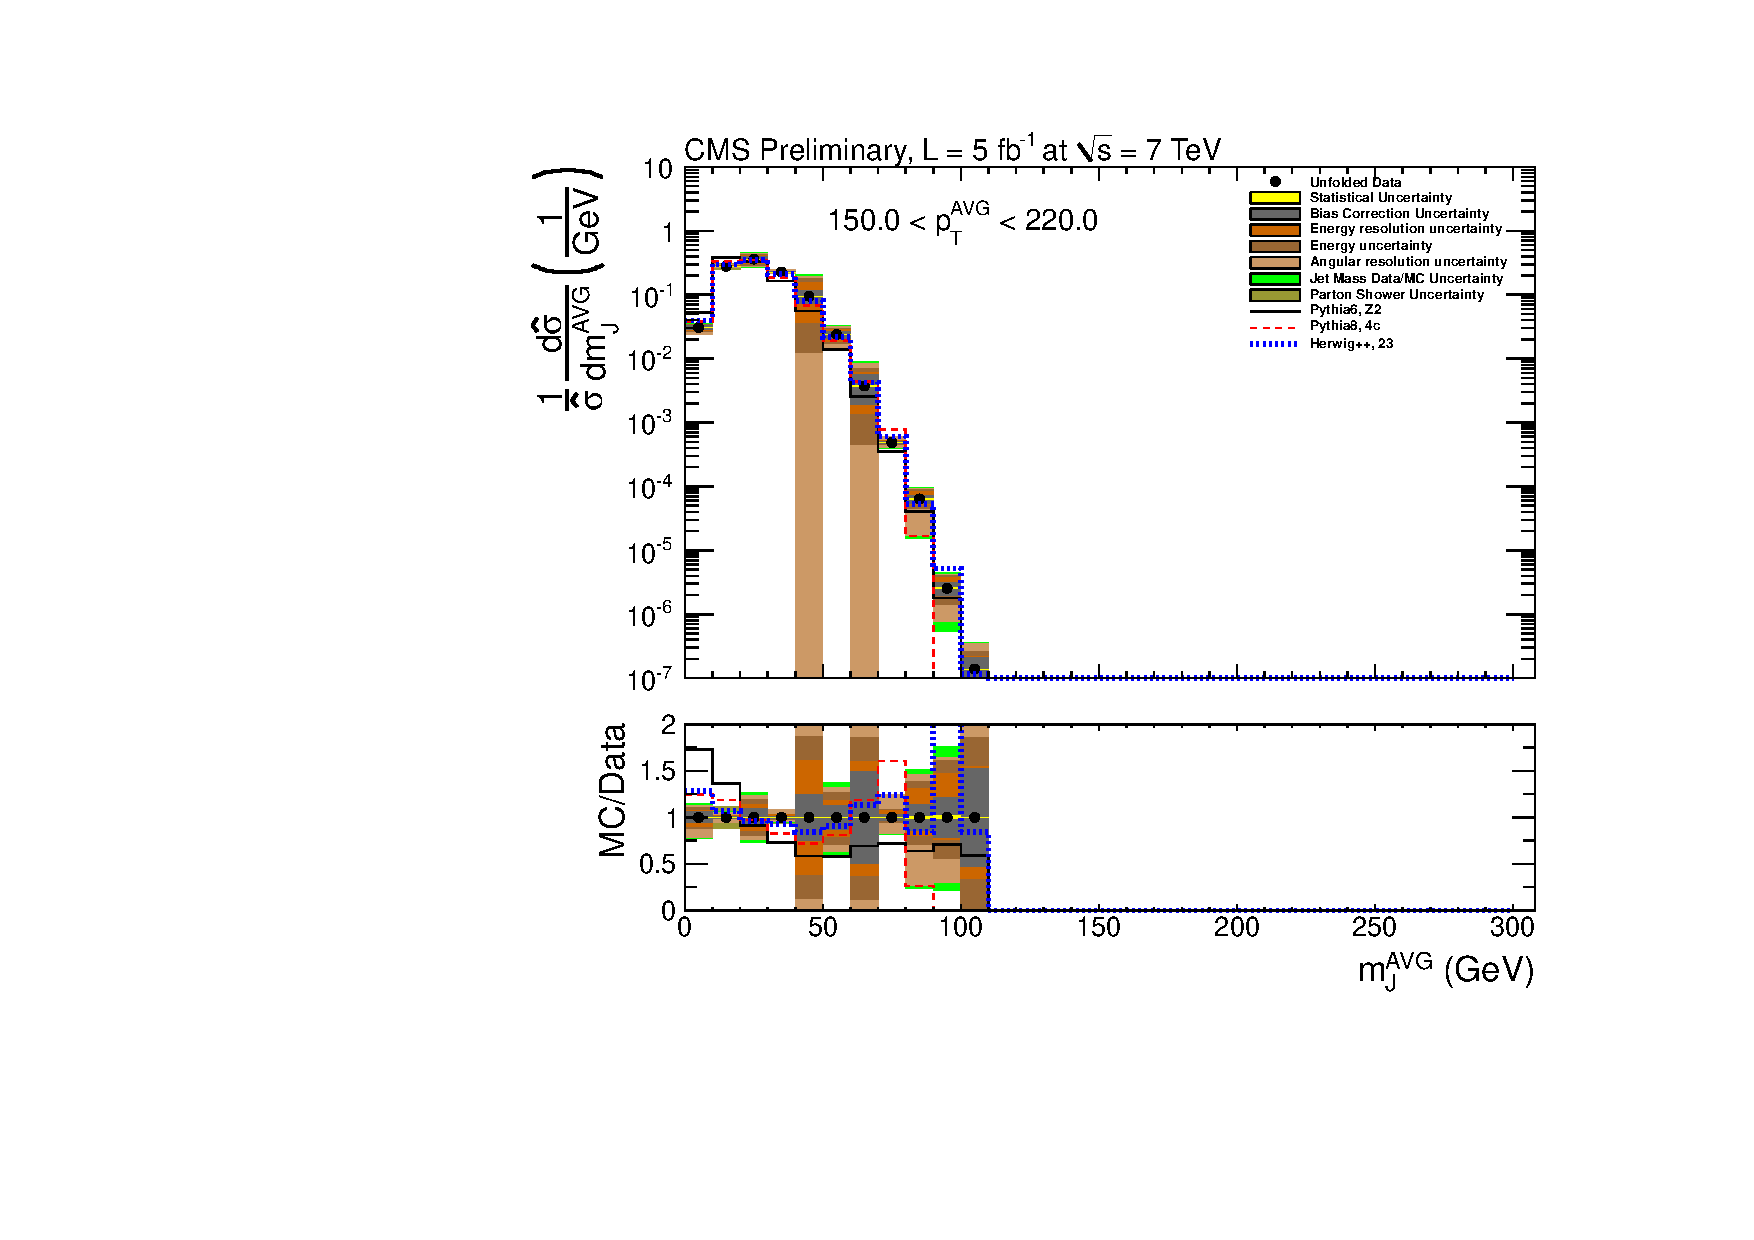
\includegraphics[width=0.95\textwidth]{figs/unfoldedMeasurementDijets_3_Trimmed_allsys}
\caption{Unfolded distributions of the jet mass for AK7 Trimmed jets,
for $150.0 < \pt^{AVG} < 220.0$ \GeVc. The data are shown in black
points. 
The statistical uncertainty is shown in light yellow, the uncertainties due to the jet-energy resolution, jet-energy scale, and jet-angular resolution are shown in shades of brown, the uncertainty due to pile-up is shown in green, and the uncertainty due to the parton shower are shown in dark yellow.
The simulated distribution from \PYTHIA is shown in solid black, 
the from \PYTHIAEIGHT in dashed red, and from \HERWIG in dotted blue. 
The bottom frame shows the ratio of the true distribution from
the simulation divided by the unfolded distribution, along with
the uncertainties in the unfolded distribution. 
\label{figs:unfoldedMeasurementDijets_3_Trimmed_allsys}}
\end{figure}



\begin{figure}[htbp]
\centering
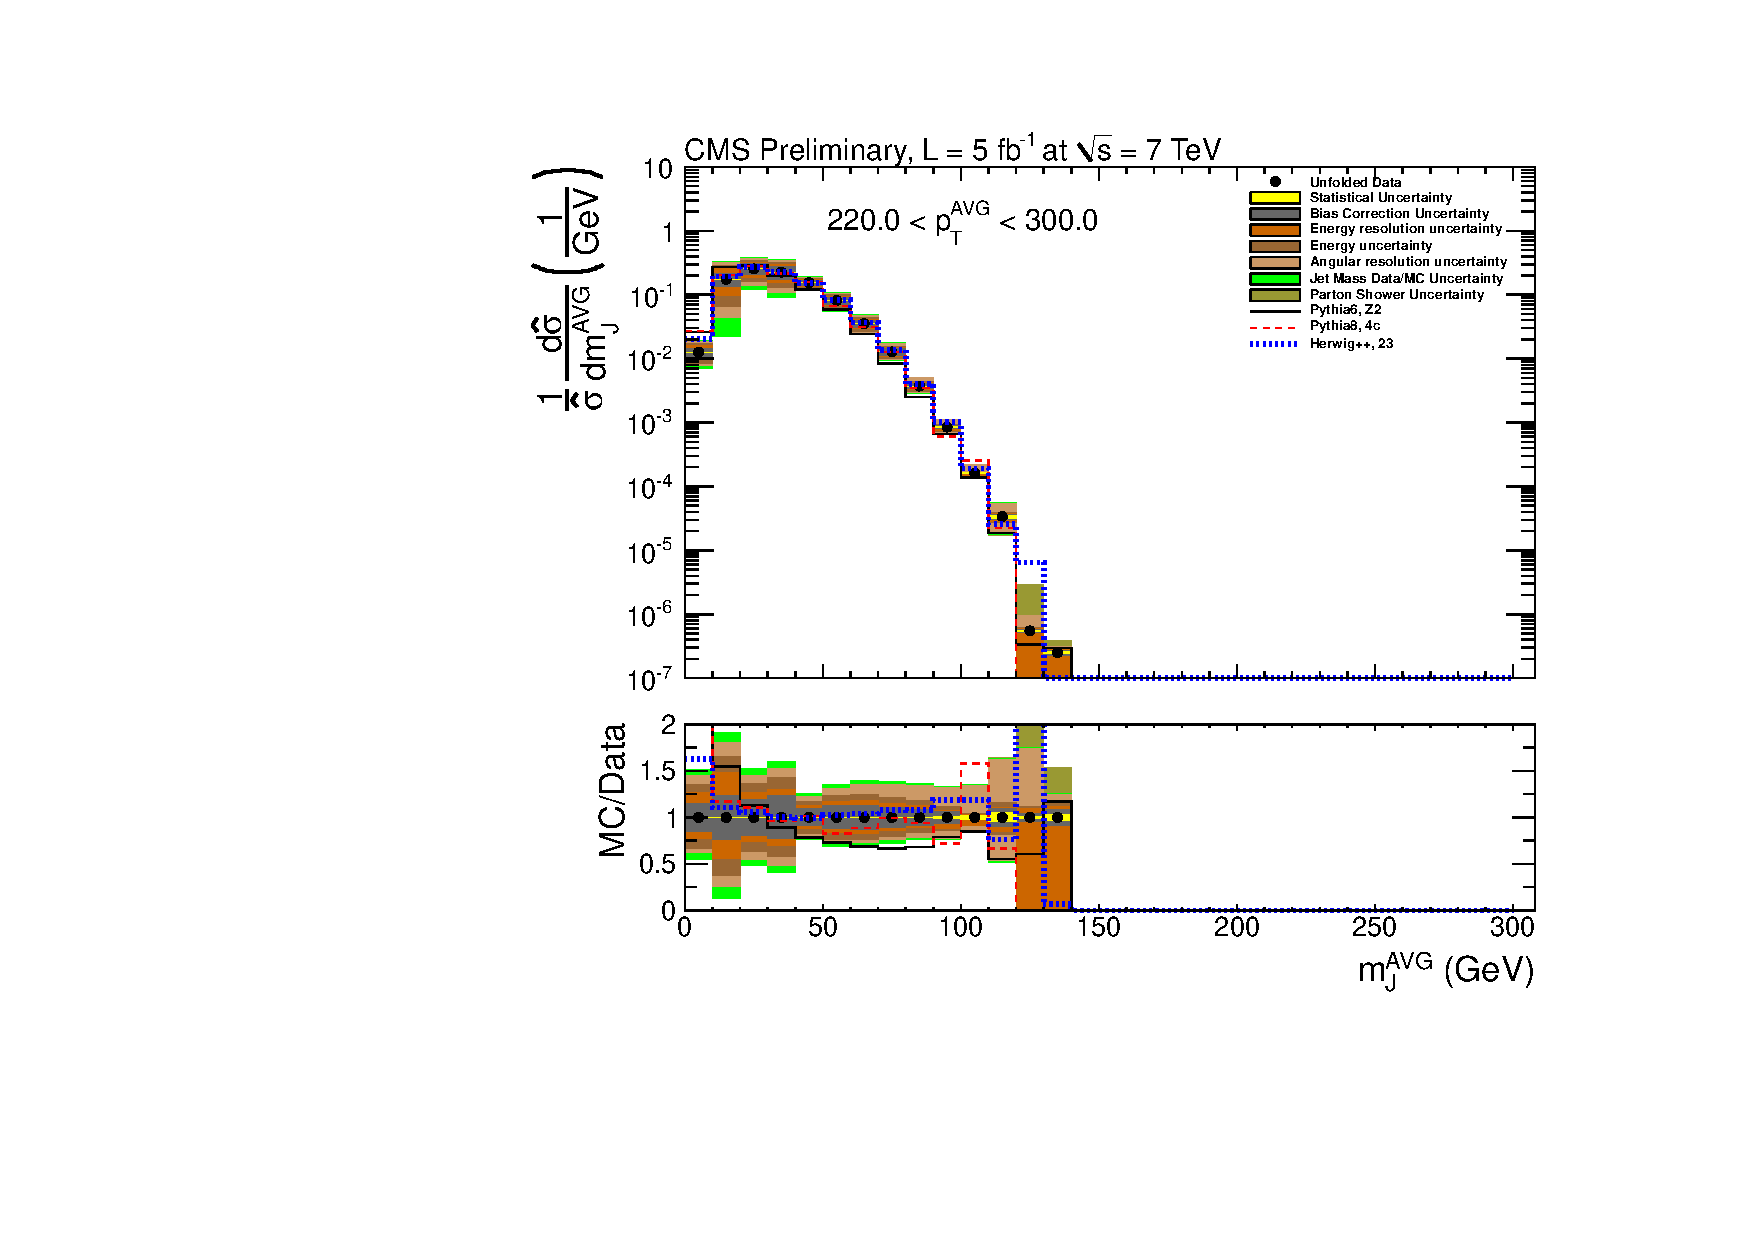
\includegraphics[width=0.95\textwidth]{figs/unfoldedMeasurementDijets_4_Trimmed_allsys}
\caption{Unfolded distributions of the jet mass for AK7 Trimmed jets,
for $220.0 < \pt^{AVG} < 300.0$ \GeVc. The data are shown in black
points. 
The statistical uncertainty is shown in light yellow, the uncertainties due to the jet-energy resolution, jet-energy scale, and jet-angular resolution are shown in shades of brown, the uncertainty due to pile-up is shown in green, and the uncertainty due to the parton shower are shown in dark yellow.
The simulated distribution from \PYTHIA is shown in solid black, 
the from \PYTHIAEIGHT in dashed red, and from \HERWIG in dotted blue. 
The bottom frame shows the ratio of the true distribution from
the simulation divided by the unfolded distribution, along with
the uncertainties in the unfolded distribution. 
\label{figs:unfoldedMeasurementDijets_4_Trimmed_allsys}}
\end{figure}



\begin{figure}[htbp]
\centering
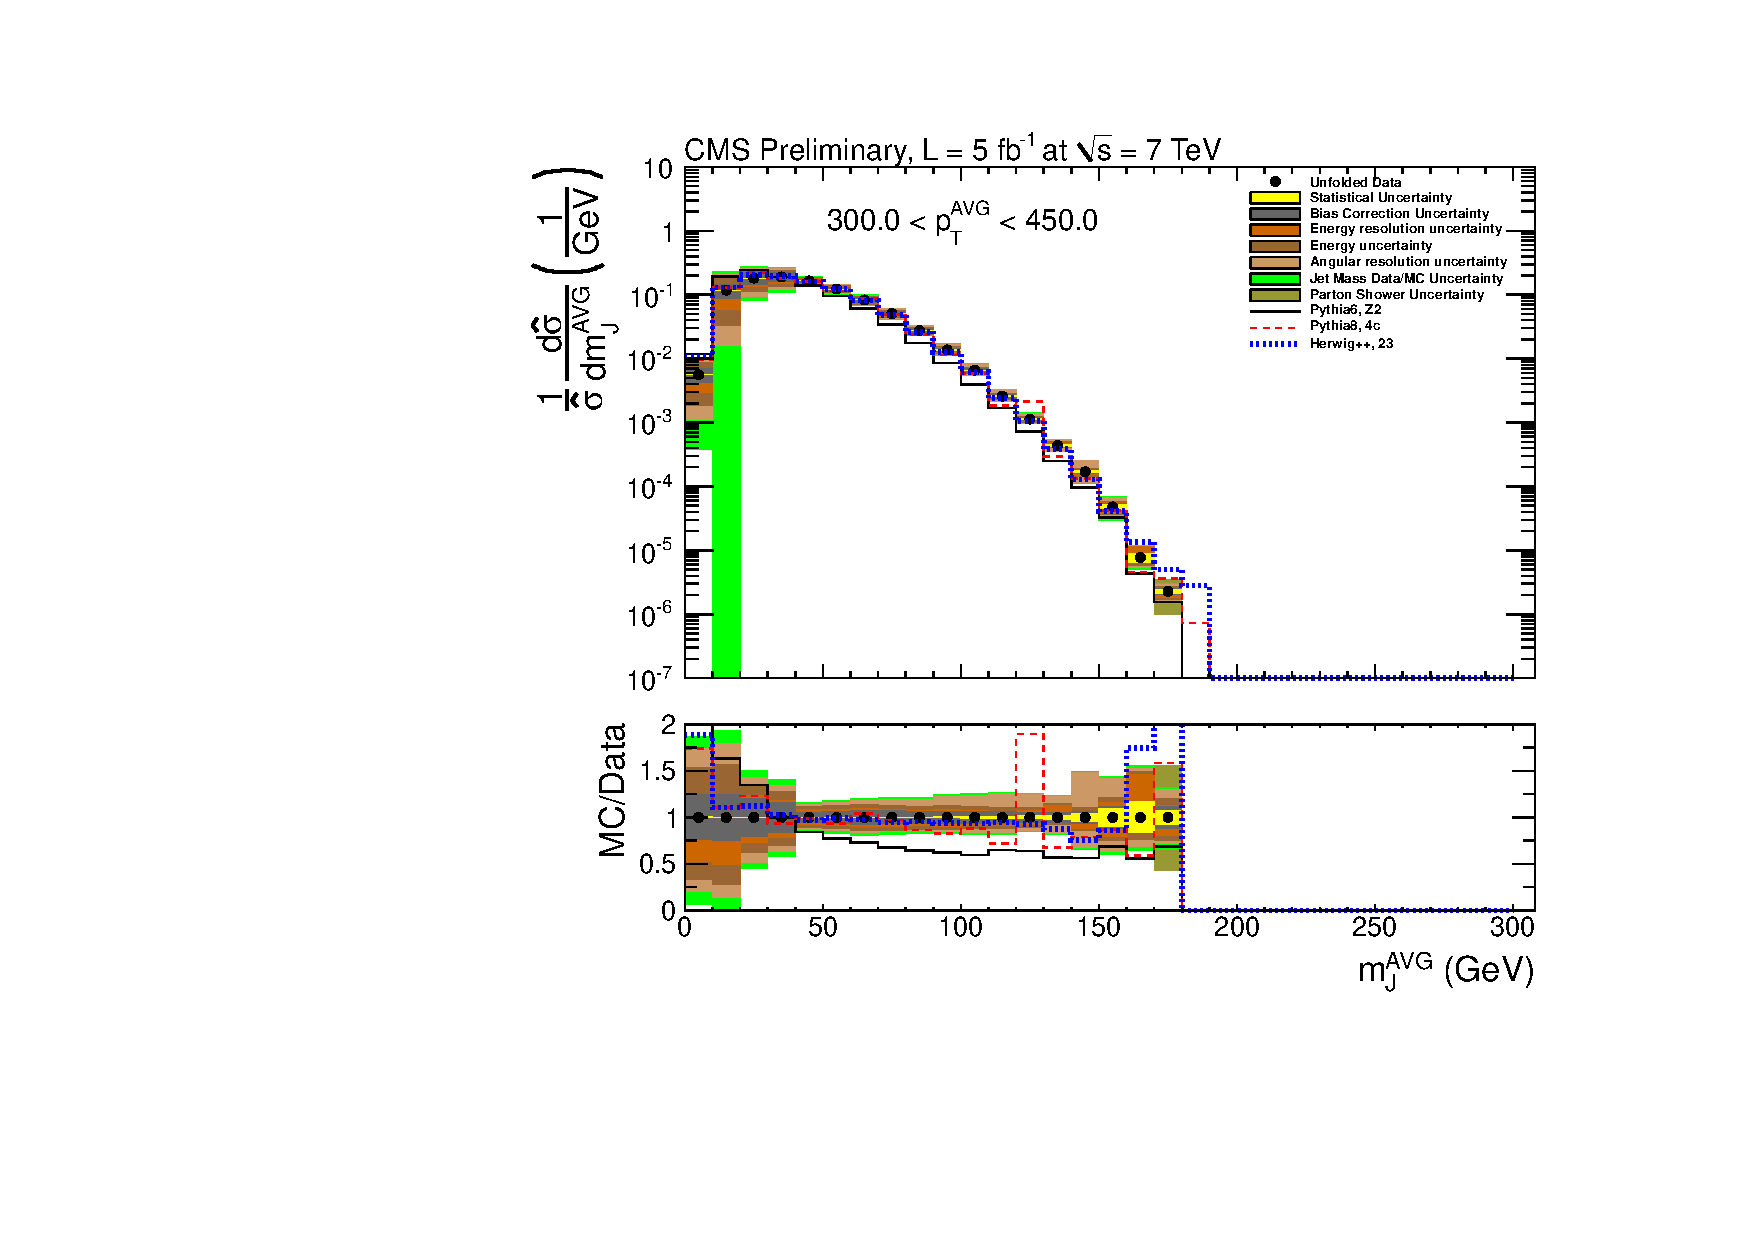
\includegraphics[width=0.95\textwidth]{figs/unfoldedMeasurementDijets_5_Trimmed_allsys}
\caption{Unfolded distributions of the jet mass for AK7 Trimmed jets,
for $300.0 < \pt^{AVG} < 450.0$ \GeVc. The data are shown in black
points. 
The statistical uncertainty is shown in light yellow, the uncertainties due to the jet-energy resolution, jet-energy scale, and jet-angular resolution are shown in shades of brown, the uncertainty due to pile-up is shown in green, and the uncertainty due to the parton shower are shown in dark yellow.
The simulated distribution from \PYTHIA is shown in solid black, 
the from \PYTHIAEIGHT in dashed red, and from \HERWIG in dotted blue. 
The bottom frame shows the ratio of the true distribution from
the simulation divided by the unfolded distribution, along with
the uncertainties in the unfolded distribution. 
\label{figs:unfoldedMeasurementDijets_5_Trimmed_allsys}}
\end{figure}



\begin{figure}[htbp]
\centering
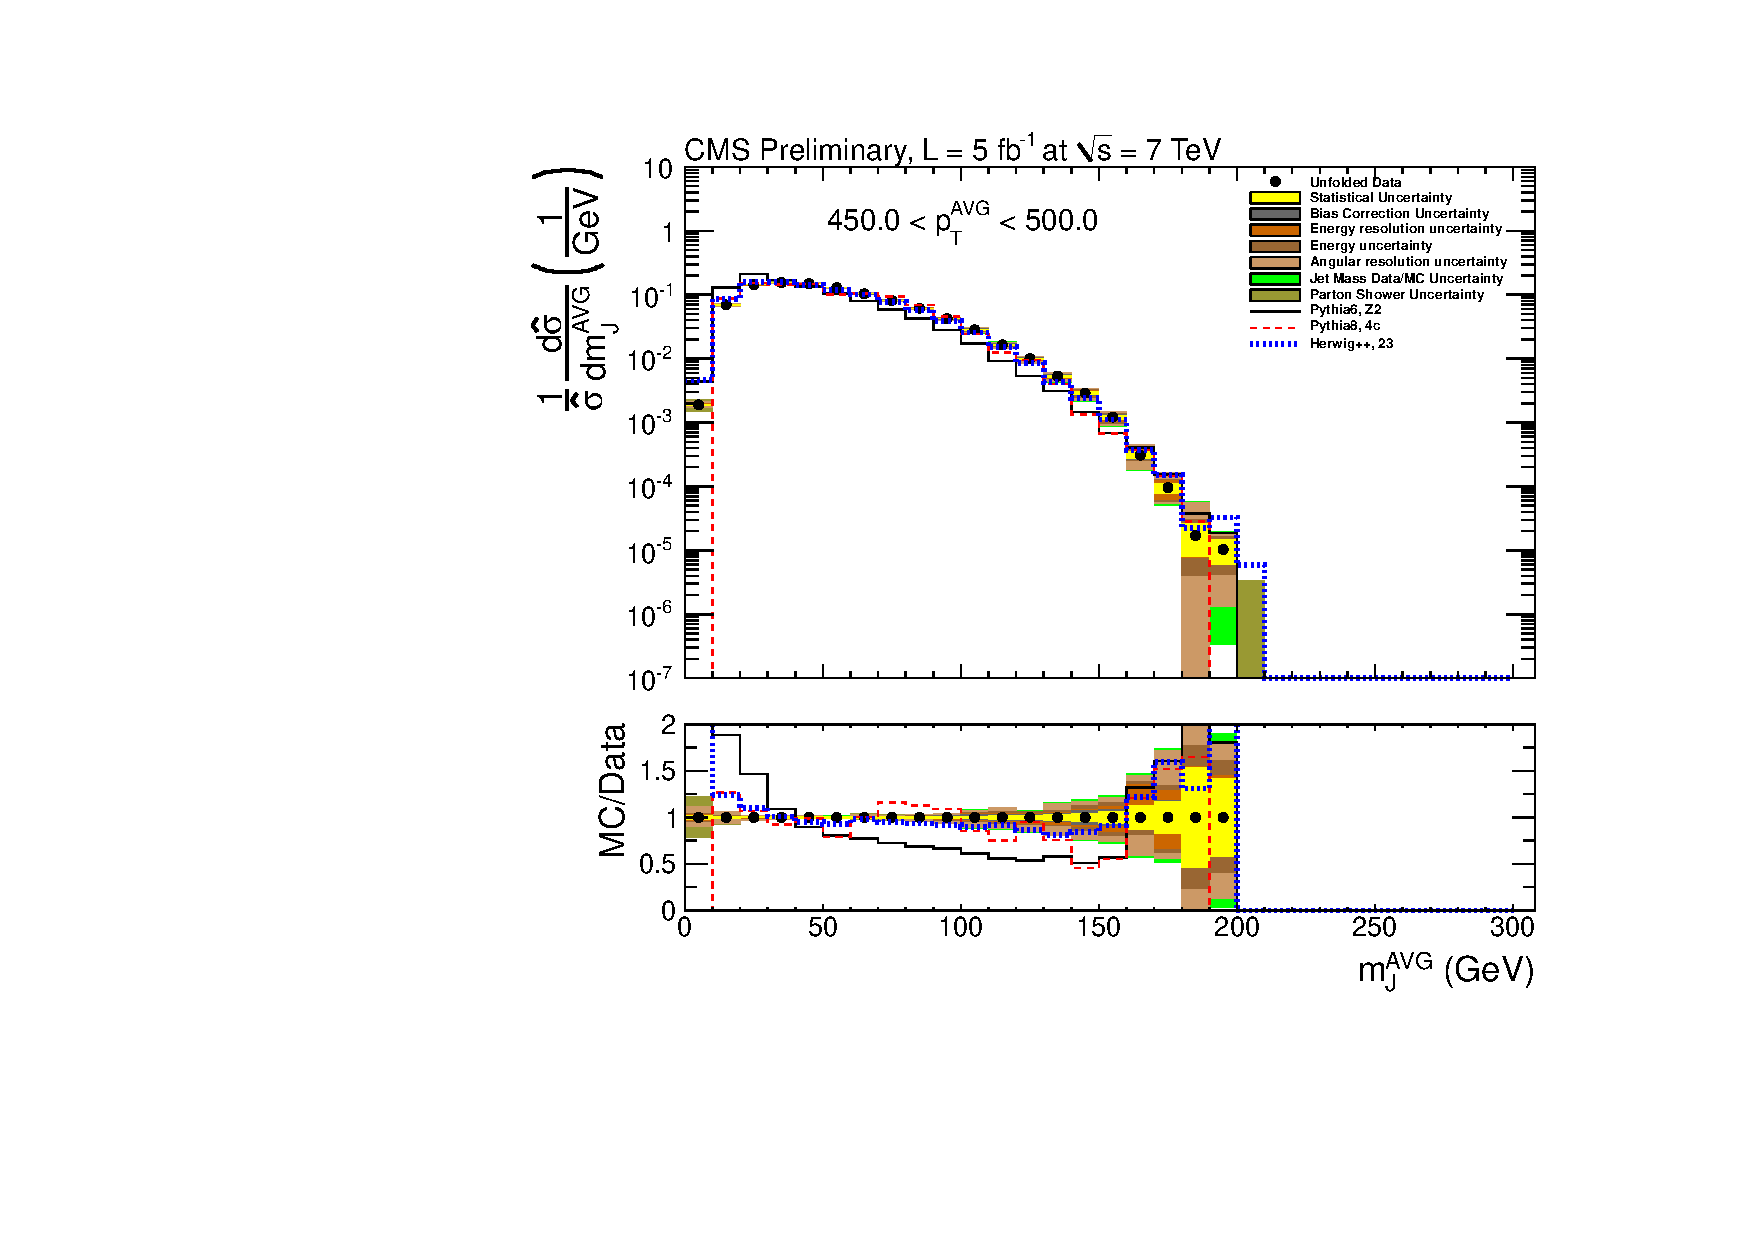
\includegraphics[width=0.95\textwidth]{figs/unfoldedMeasurementDijets_6_Trimmed_allsys}
\caption{Unfolded distributions of the jet mass for AK7 Trimmed jets,
for $450.0 < \pt^{AVG} < 500.0$ \GeVc. The data are shown in black
points. 
The statistical uncertainty is shown in light yellow, the uncertainties due to the jet-energy resolution, jet-energy scale, and jet-angular resolution are shown in shades of brown, the uncertainty due to pile-up is shown in green, and the uncertainty due to the parton shower are shown in dark yellow.
The simulated distribution from \PYTHIA is shown in solid black, 
the from \PYTHIAEIGHT in dashed red, and from \HERWIG in dotted blue. 
The bottom frame shows the ratio of the true distribution from
the simulation divided by the unfolded distribution, along with
the uncertainties in the unfolded distribution. 
\label{figs:unfoldedMeasurementDijets_6_Trimmed_allsys}}
\end{figure}



\begin{figure}[htbp]
\centering
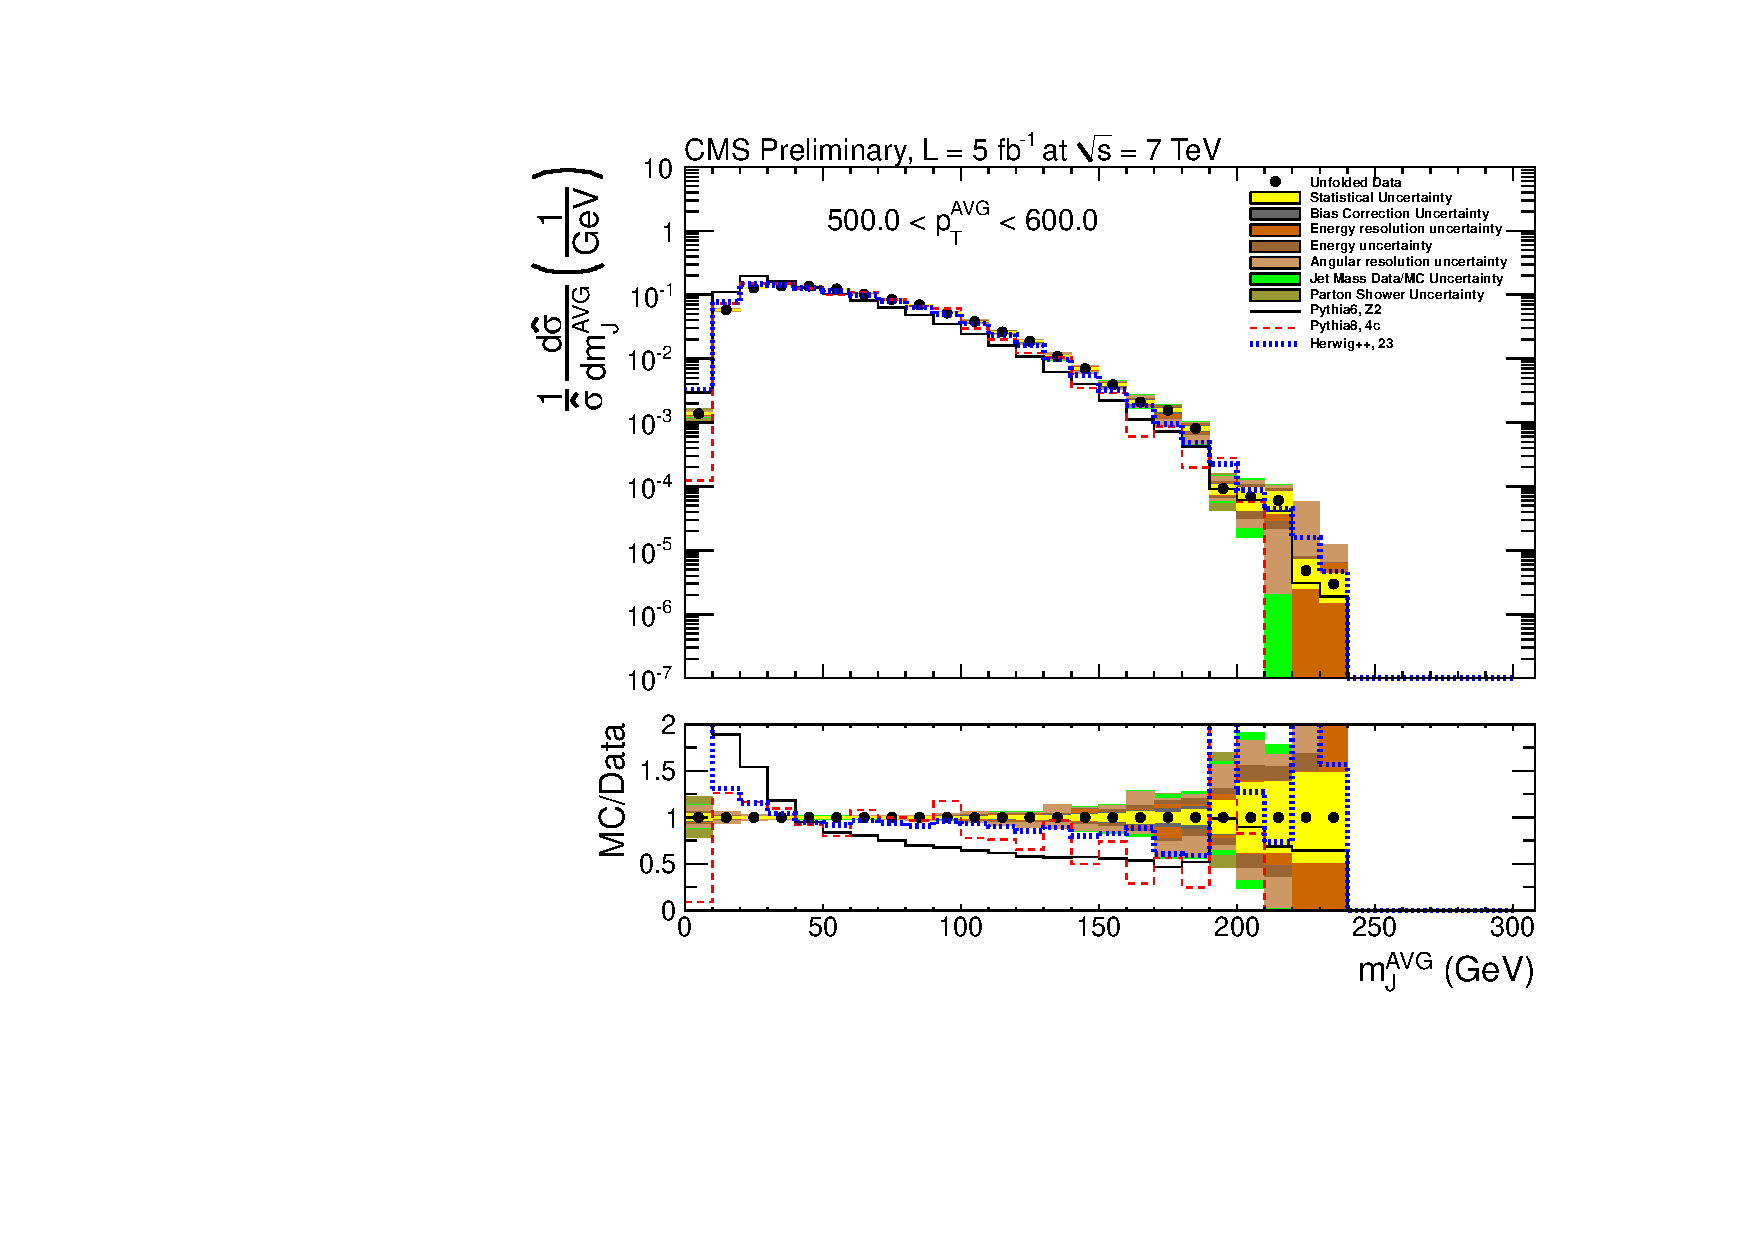
\includegraphics[width=0.95\textwidth]{figs/unfoldedMeasurementDijets_7_Trimmed_allsys}
\caption{Unfolded distributions of the jet mass for AK7 Trimmed jets,
for $500.0 < \pt^{AVG} < 600.0$ \GeVc. The data are shown in black
points. 
The statistical uncertainty is shown in light yellow, the uncertainties due to the jet-energy resolution, jet-energy scale, and jet-angular resolution are shown in shades of brown, the uncertainty due to pile-up is shown in green, and the uncertainty due to the parton shower are shown in dark yellow.
The simulated distribution from \PYTHIA is shown in solid black, 
the from \PYTHIAEIGHT in dashed red, and from \HERWIG in dotted blue. 
The bottom frame shows the ratio of the true distribution from
the simulation divided by the unfolded distribution, along with
the uncertainties in the unfolded distribution. 
\label{figs:unfoldedMeasurementDijets_7_Trimmed_allsys}}
\end{figure}



\begin{figure}[htbp]
\centering
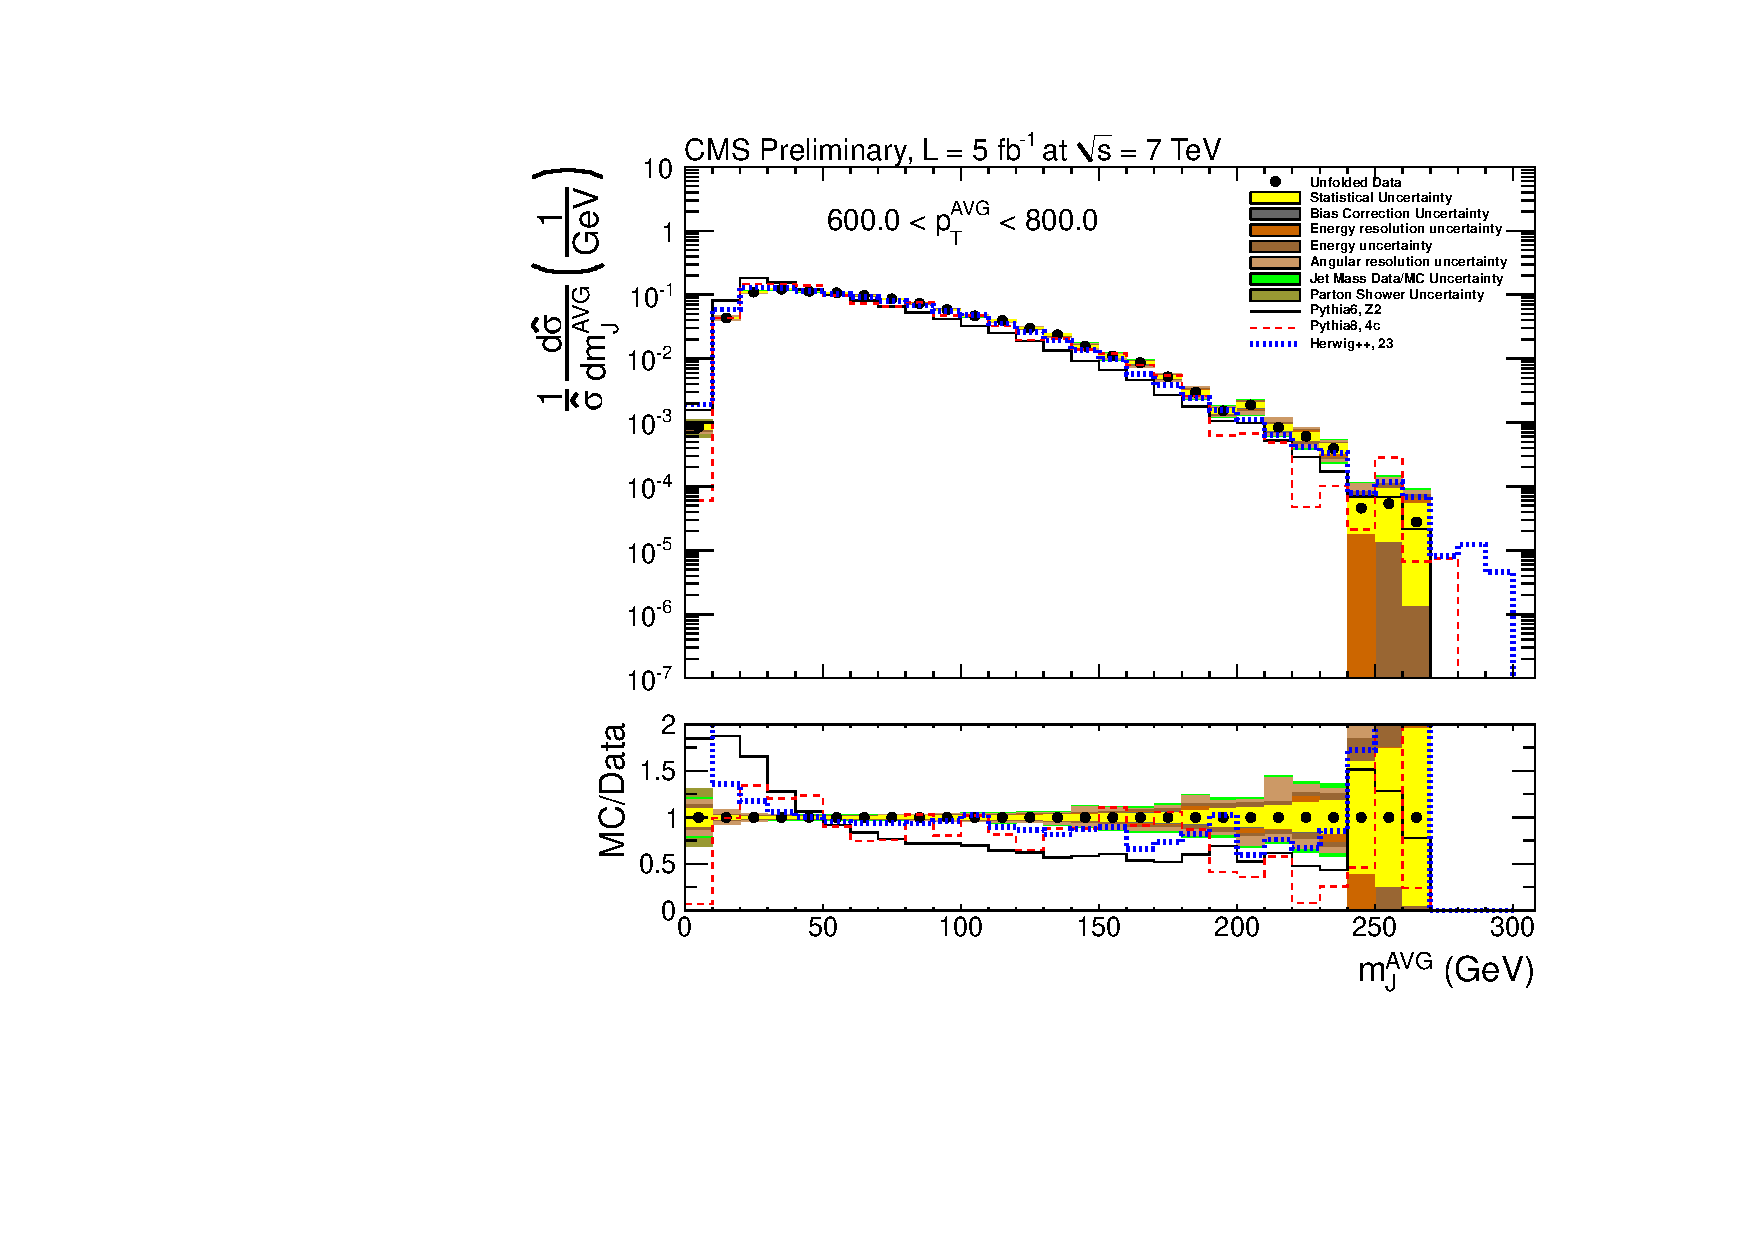
\includegraphics[width=0.95\textwidth]{figs/unfoldedMeasurementDijets_8_Trimmed_allsys}
\caption{Unfolded distributions of the jet mass for AK7 Trimmed jets,
for $600.0 < \pt^{AVG} < 800.0$ \GeVc. The data are shown in black
points. 
The statistical uncertainty is shown in light yellow, the uncertainties due to the jet-energy resolution, jet-energy scale, and jet-angular resolution are shown in shades of brown, the uncertainty due to pile-up is shown in green, and the uncertainty due to the parton shower are shown in dark yellow.
The simulated distribution from \PYTHIA is shown in solid black, 
the from \PYTHIAEIGHT in dashed red, and from \HERWIG in dotted blue. 
The bottom frame shows the ratio of the true distribution from
the simulation divided by the unfolded distribution, along with
the uncertainties in the unfolded distribution. 
\label{figs:unfoldedMeasurementDijets_8_Trimmed_allsys}}
\end{figure}



\begin{figure}[htbp]
\centering
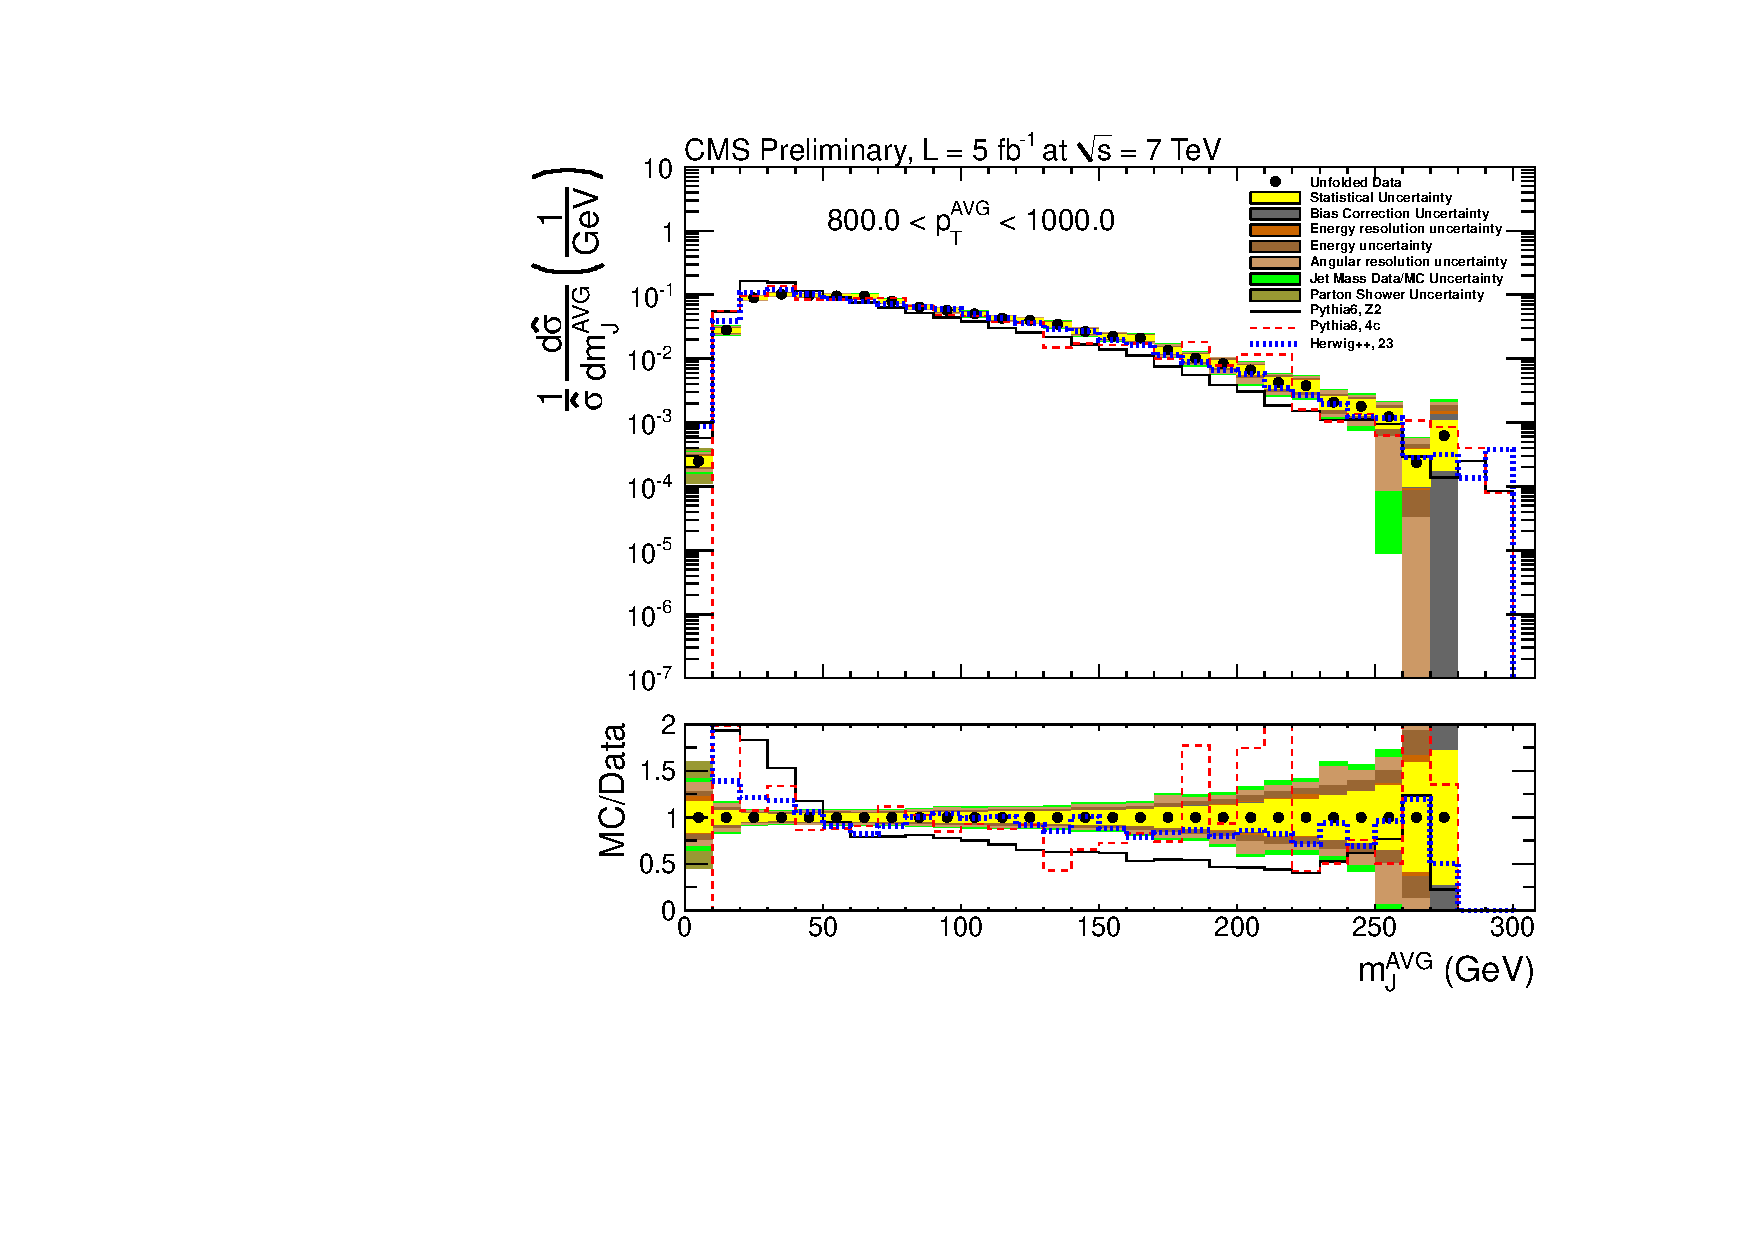
\includegraphics[width=0.95\textwidth]{figs/unfoldedMeasurementDijets_9_Trimmed_allsys}
\caption{Unfolded distributions of the jet mass for AK7 Trimmed jets,
for $800.0 < \pt^{AVG} < 1000.0$ \GeVc. The data are shown in black
points. 
The statistical uncertainty is shown in light yellow, the uncertainties due to the jet-energy resolution, jet-energy scale, and jet-angular resolution are shown in shades of brown, the uncertainty due to pile-up is shown in green, and the uncertainty due to the parton shower are shown in dark yellow.
The simulated distribution from \PYTHIA is shown in solid black, 
the from \PYTHIAEIGHT in dashed red, and from \HERWIG in dotted blue. 
The bottom frame shows the ratio of the true distribution from
the simulation divided by the unfolded distribution, along with
the uncertainties in the unfolded distribution. 
\label{figs:unfoldedMeasurementDijets_9_Trimmed_allsys}}
\end{figure}



\begin{figure}[htbp]
\centering
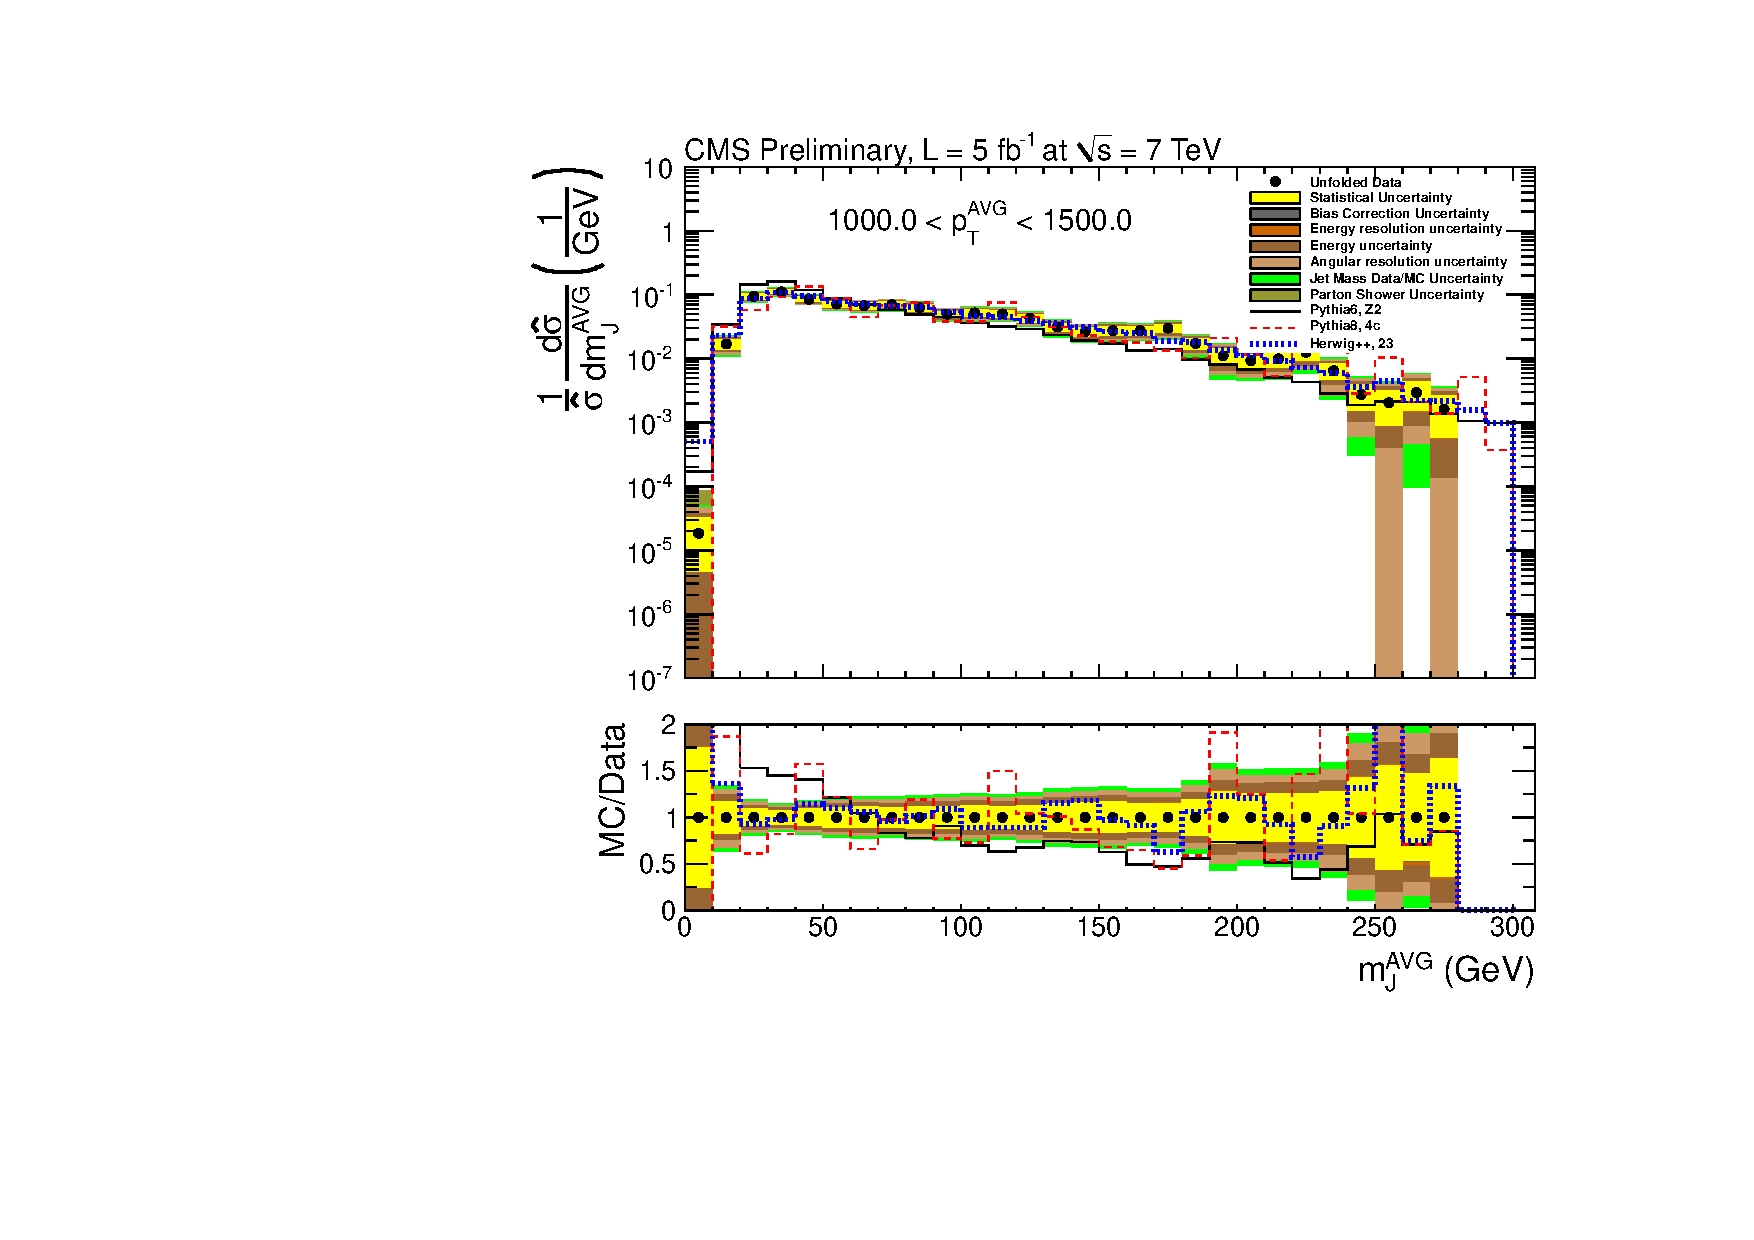
\includegraphics[width=0.95\textwidth]{figs/unfoldedMeasurementDijets_10_Trimmed_allsys}
\caption{Unfolded distributions of the jet mass for AK7 Trimmed jets,
for $1000.0 < \pt^{AVG} < 1500.0$ \GeVc. The data are shown in black
points. 
The statistical uncertainty is shown in light yellow, the uncertainties due to the jet-energy resolution, jet-energy scale, and jet-angular resolution are shown in shades of brown, the uncertainty due to pile-up is shown in green, and the uncertainty due to the parton shower are shown in dark yellow.
The simulated distribution from \PYTHIA is shown in solid black, 
the from \PYTHIAEIGHT in dashed red, and from \HERWIG in dotted blue. 
The bottom frame shows the ratio of the true distribution from
the simulation divided by the unfolded distribution, along with
the uncertainties in the unfolded distribution. 
\label{figs:unfoldedMeasurementDijets_10_Trimmed_allsys}}
\end{figure}

\clearpage

\begin{figure}[htbp]
\centering
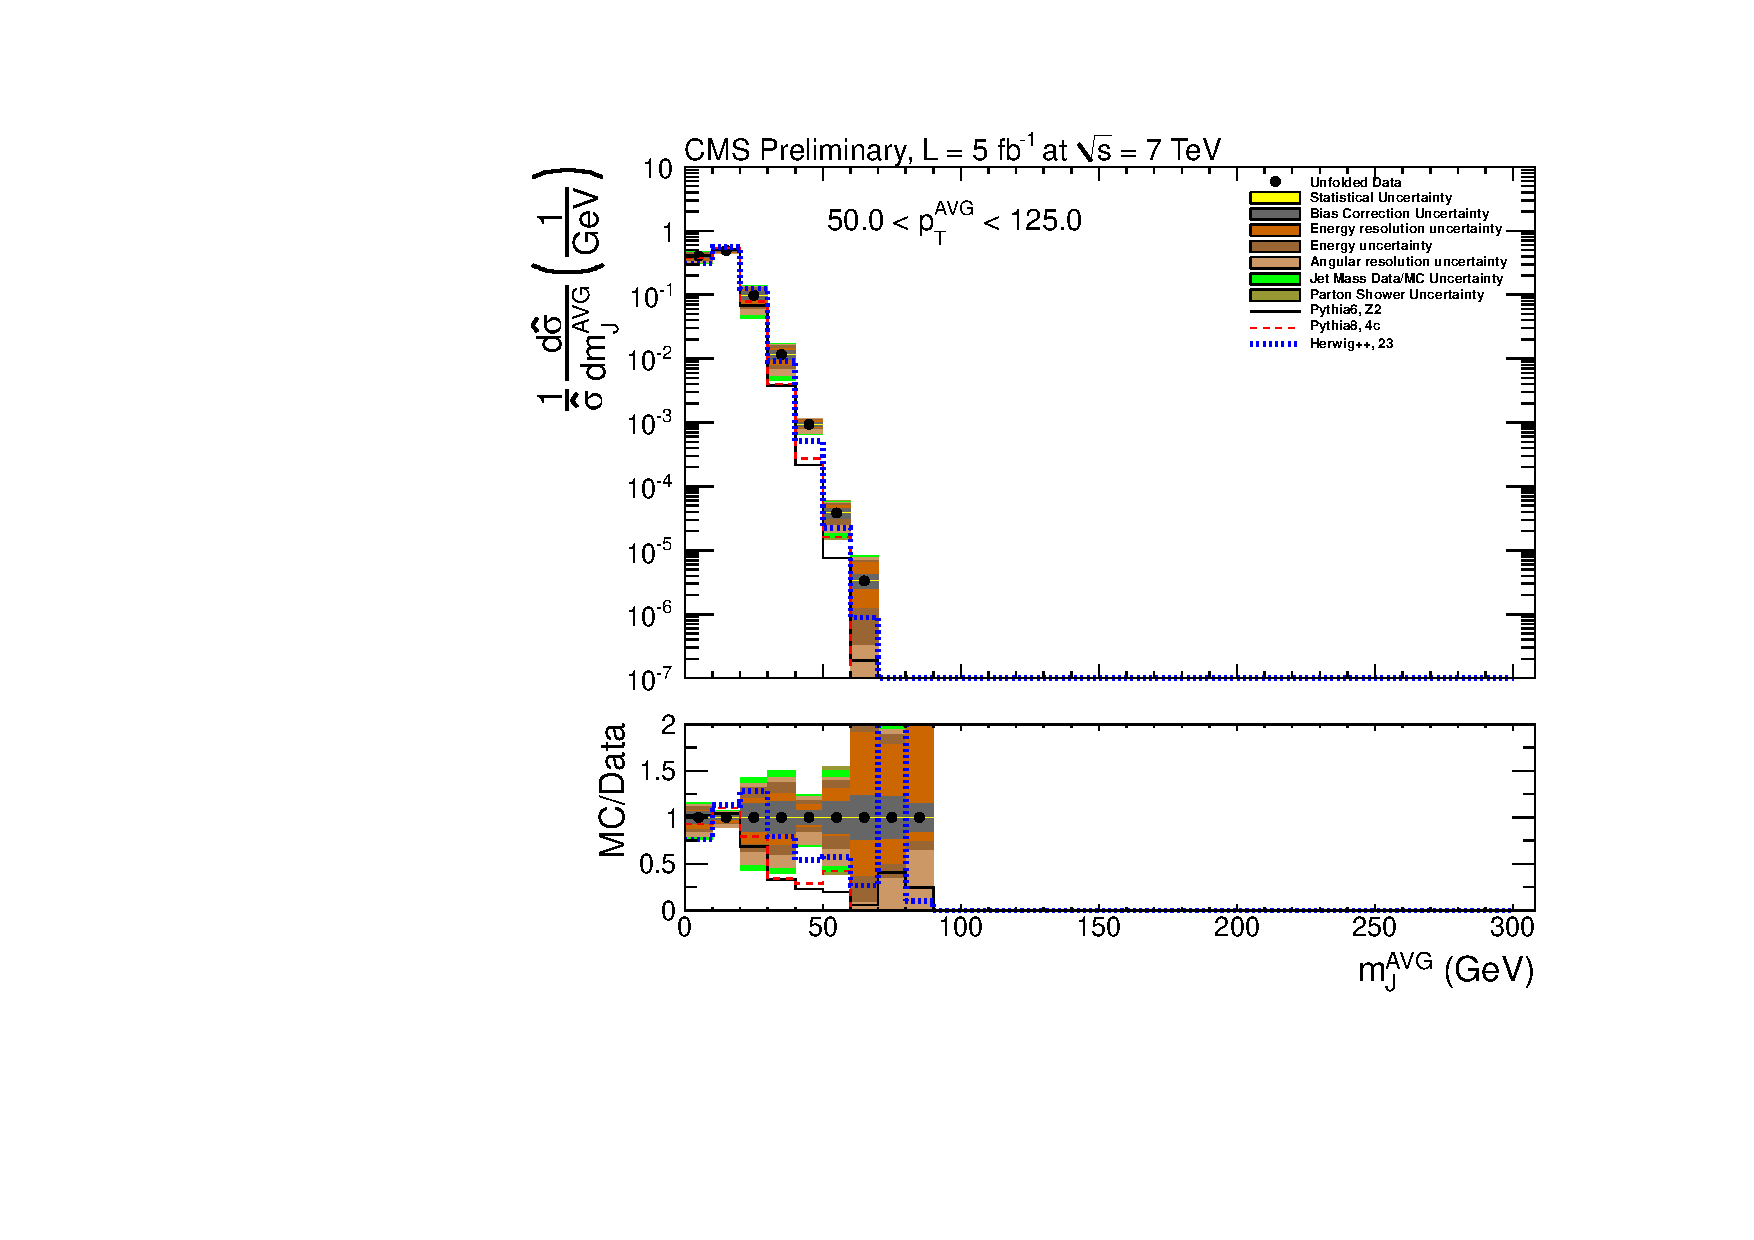
\includegraphics[width=0.95\textwidth]{figs/unfoldedMeasurementDijets_1_Pruned_allsys}
\caption{Unfolded distributions of the jet mass for AK7 Pruned jets,
for $50.0 < \pt^{AVG} < 125.0$ \GeVc. The data are shown in black
points. 
The statistical uncertainty is shown in light yellow, the uncertainties due to the jet-energy resolution, jet-energy scale, and jet-angular resolution are shown in shades of brown, the uncertainty due to pile-up is shown in green, and the uncertainty due to the parton shower are shown in dark yellow.
The simulated distribution from \PYTHIA is shown in solid black, 
the from \PYTHIAEIGHT in dashed red, and from \HERWIG in dotted blue. 
The bottom frame shows the ratio of the true distribution from
the simulation divided by the unfolded distribution, along with
the uncertainties in the unfolded distribution. 
\label{figs:unfoldedMeasurementDijets_1_Pruned_allsys}}
\end{figure}



\begin{figure}[htbp]
\centering
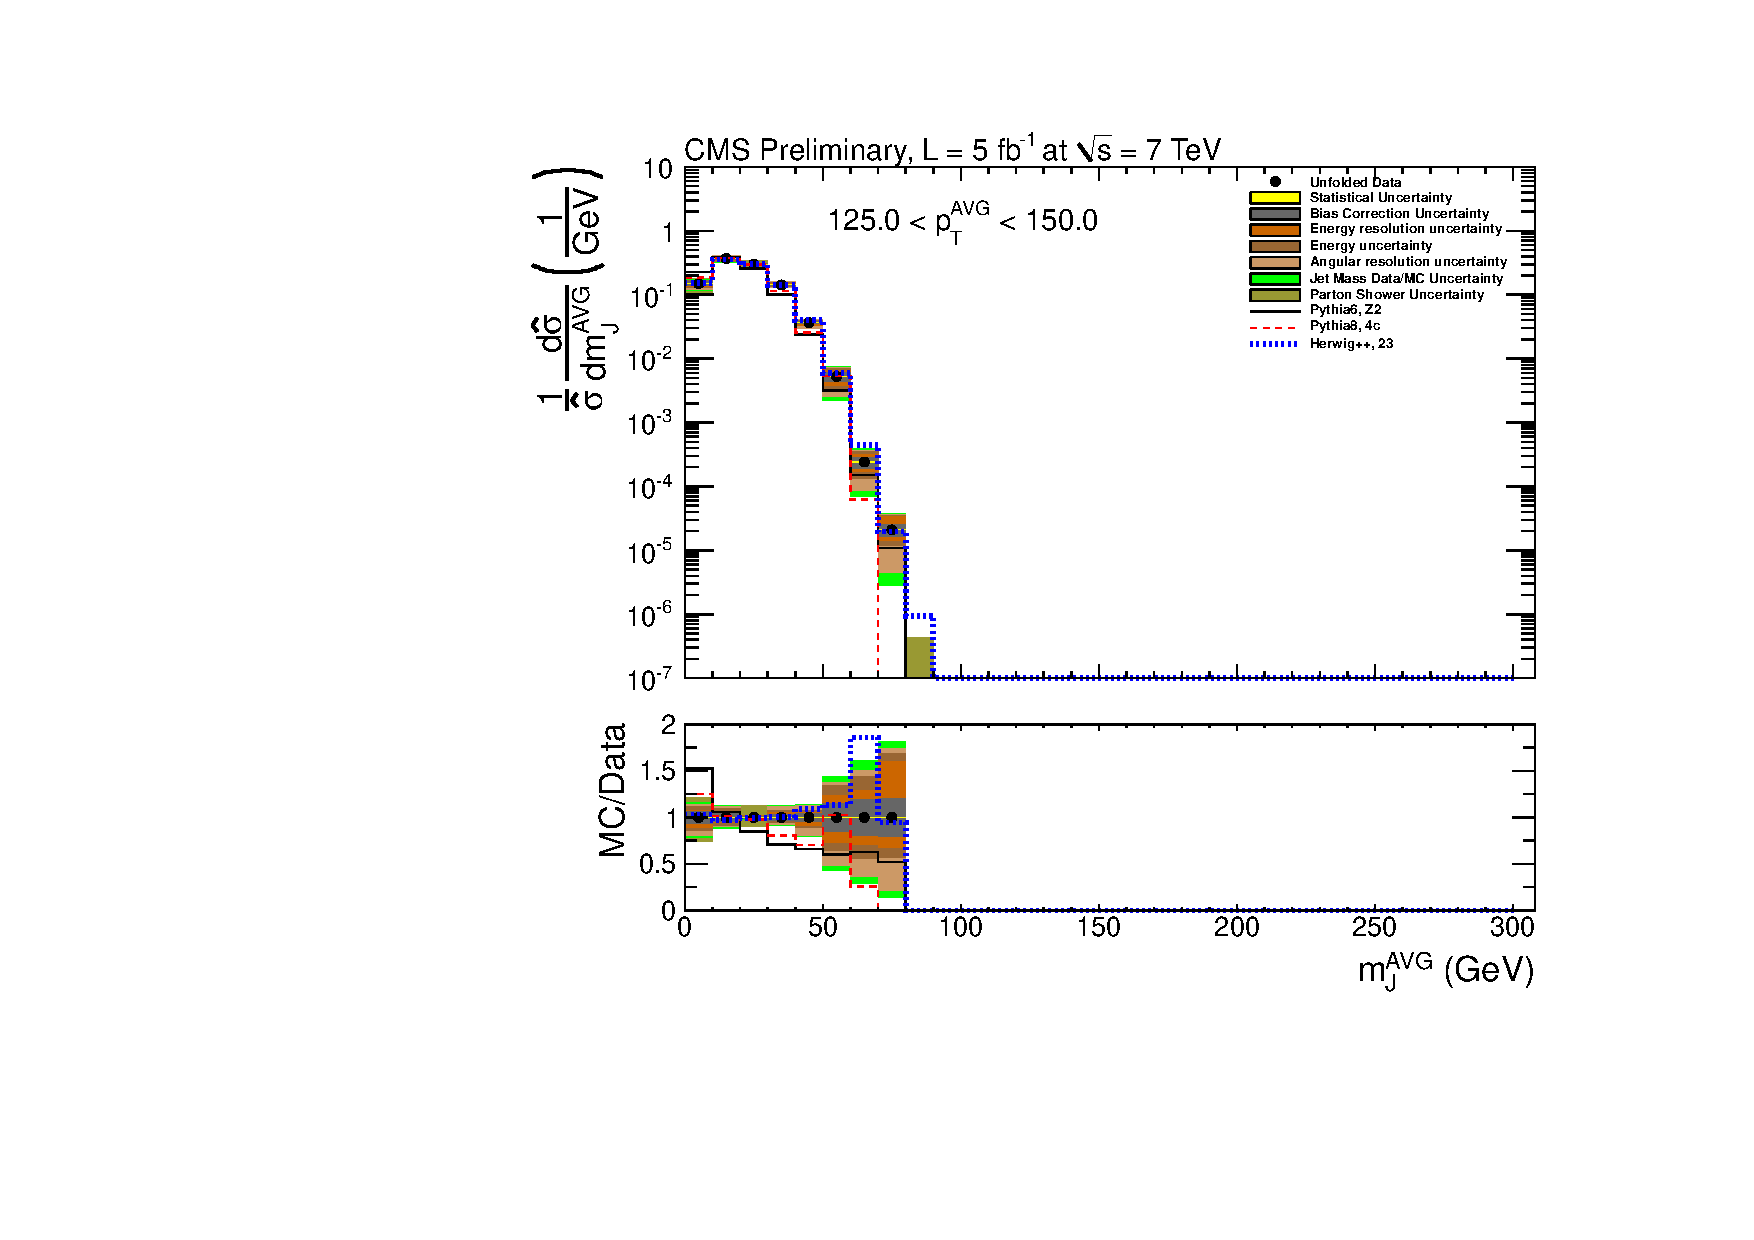
\includegraphics[width=0.95\textwidth]{figs/unfoldedMeasurementDijets_2_Pruned_allsys}
\caption{Unfolded distributions of the jet mass for AK7 Pruned jets,
for $125.0 < \pt^{AVG} < 150.0$ \GeVc. The data are shown in black
points. 
The statistical uncertainty is shown in light yellow, the uncertainties due to the jet-energy resolution, jet-energy scale, and jet-angular resolution are shown in shades of brown, the uncertainty due to pile-up is shown in green, and the uncertainty due to the parton shower are shown in dark yellow.
The simulated distribution from \PYTHIA is shown in solid black, 
the from \PYTHIAEIGHT in dashed red, and from \HERWIG in dotted blue. 
The bottom frame shows the ratio of the true distribution from
the simulation divided by the unfolded distribution, along with
the uncertainties in the unfolded distribution. 
\label{figs:unfoldedMeasurementDijets_2_Pruned_allsys}}
\end{figure}



\begin{figure}[htbp]
\centering
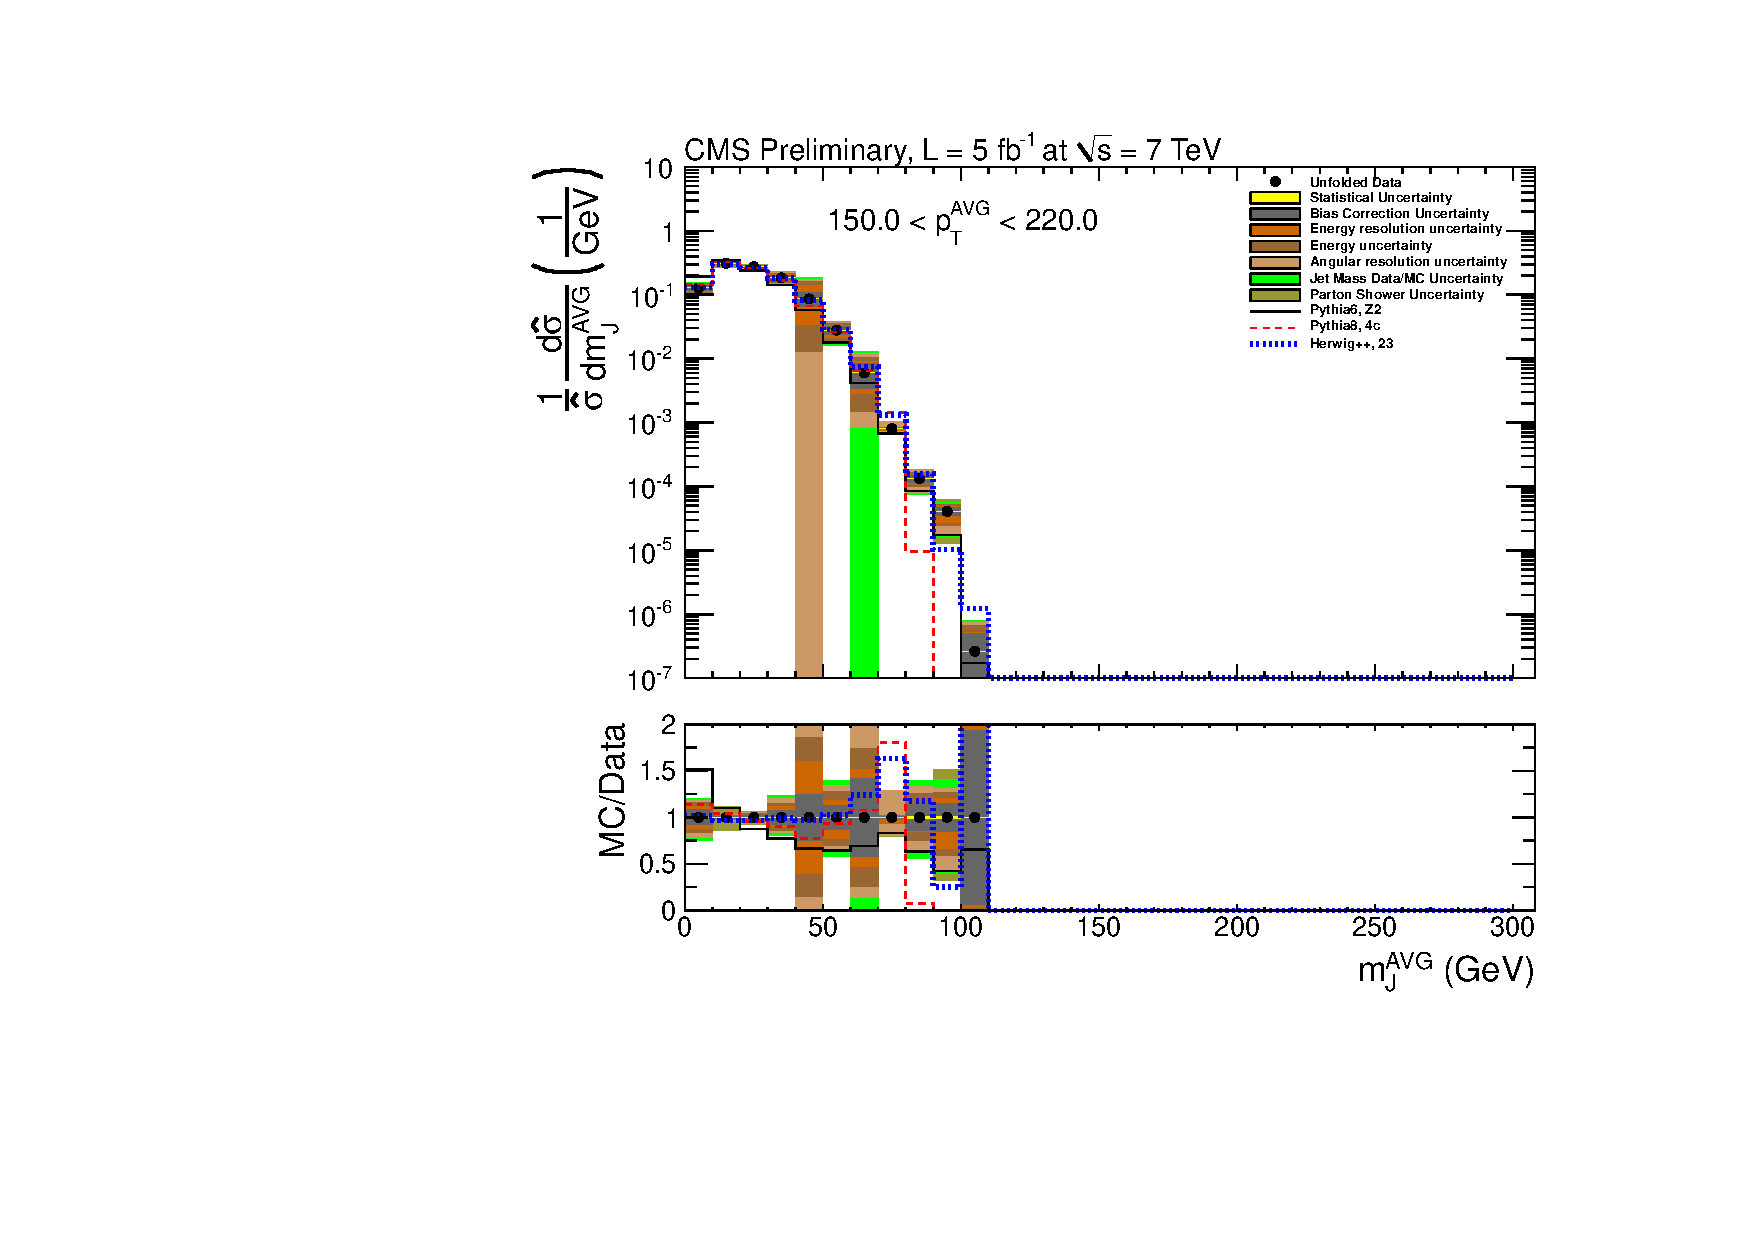
\includegraphics[width=0.95\textwidth]{figs/unfoldedMeasurementDijets_3_Pruned_allsys}
\caption{Unfolded distributions of the jet mass for AK7 Pruned jets,
for $150.0 < \pt^{AVG} < 220.0$ \GeVc. The data are shown in black
points. 
The statistical uncertainty is shown in light yellow, the uncertainties due to the jet-energy resolution, jet-energy scale, and jet-angular resolution are shown in shades of brown, the uncertainty due to pile-up is shown in green, and the uncertainty due to the parton shower are shown in dark yellow.
The simulated distribution from \PYTHIA is shown in solid black, 
the from \PYTHIAEIGHT in dashed red, and from \HERWIG in dotted blue. 
The bottom frame shows the ratio of the true distribution from
the simulation divided by the unfolded distribution, along with
the uncertainties in the unfolded distribution. 
\label{figs:unfoldedMeasurementDijets_3_Pruned_allsys}}
\end{figure}



\begin{figure}[htbp]
\centering
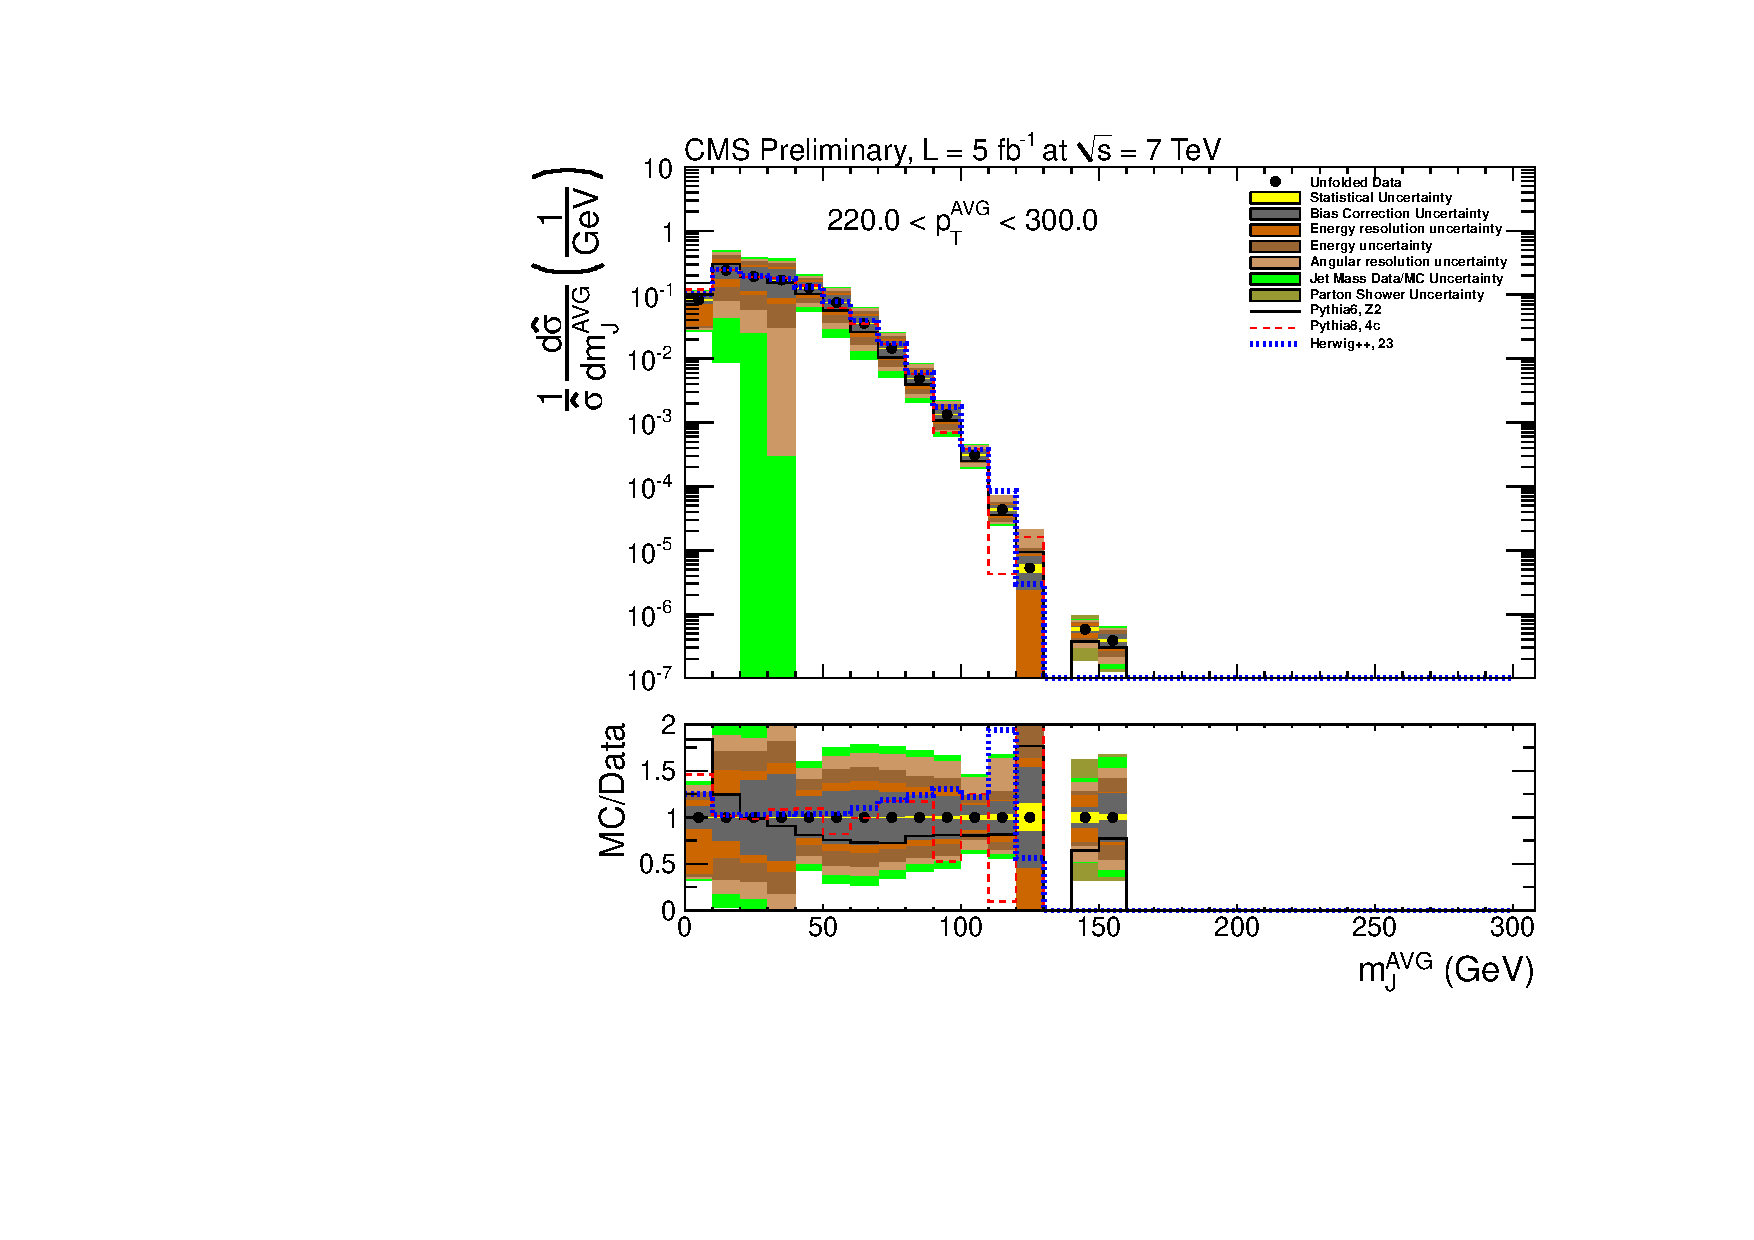
\includegraphics[width=0.95\textwidth]{figs/unfoldedMeasurementDijets_4_Pruned_allsys}
\caption{Unfolded distributions of the jet mass for AK7 Pruned jets,
for $220.0 < \pt^{AVG} < 300.0$ \GeVc. The data are shown in black
points. 
The statistical uncertainty is shown in light yellow, the uncertainties due to the jet-energy resolution, jet-energy scale, and jet-angular resolution are shown in shades of brown, the uncertainty due to pile-up is shown in green, and the uncertainty due to the parton shower are shown in dark yellow.
The simulated distribution from \PYTHIA is shown in solid black, 
the from \PYTHIAEIGHT in dashed red, and from \HERWIG in dotted blue. 
The bottom frame shows the ratio of the true distribution from
the simulation divided by the unfolded distribution, along with
the uncertainties in the unfolded distribution. 
\label{figs:unfoldedMeasurementDijets_4_Pruned_allsys}}
\end{figure}



\begin{figure}[htbp]
\centering
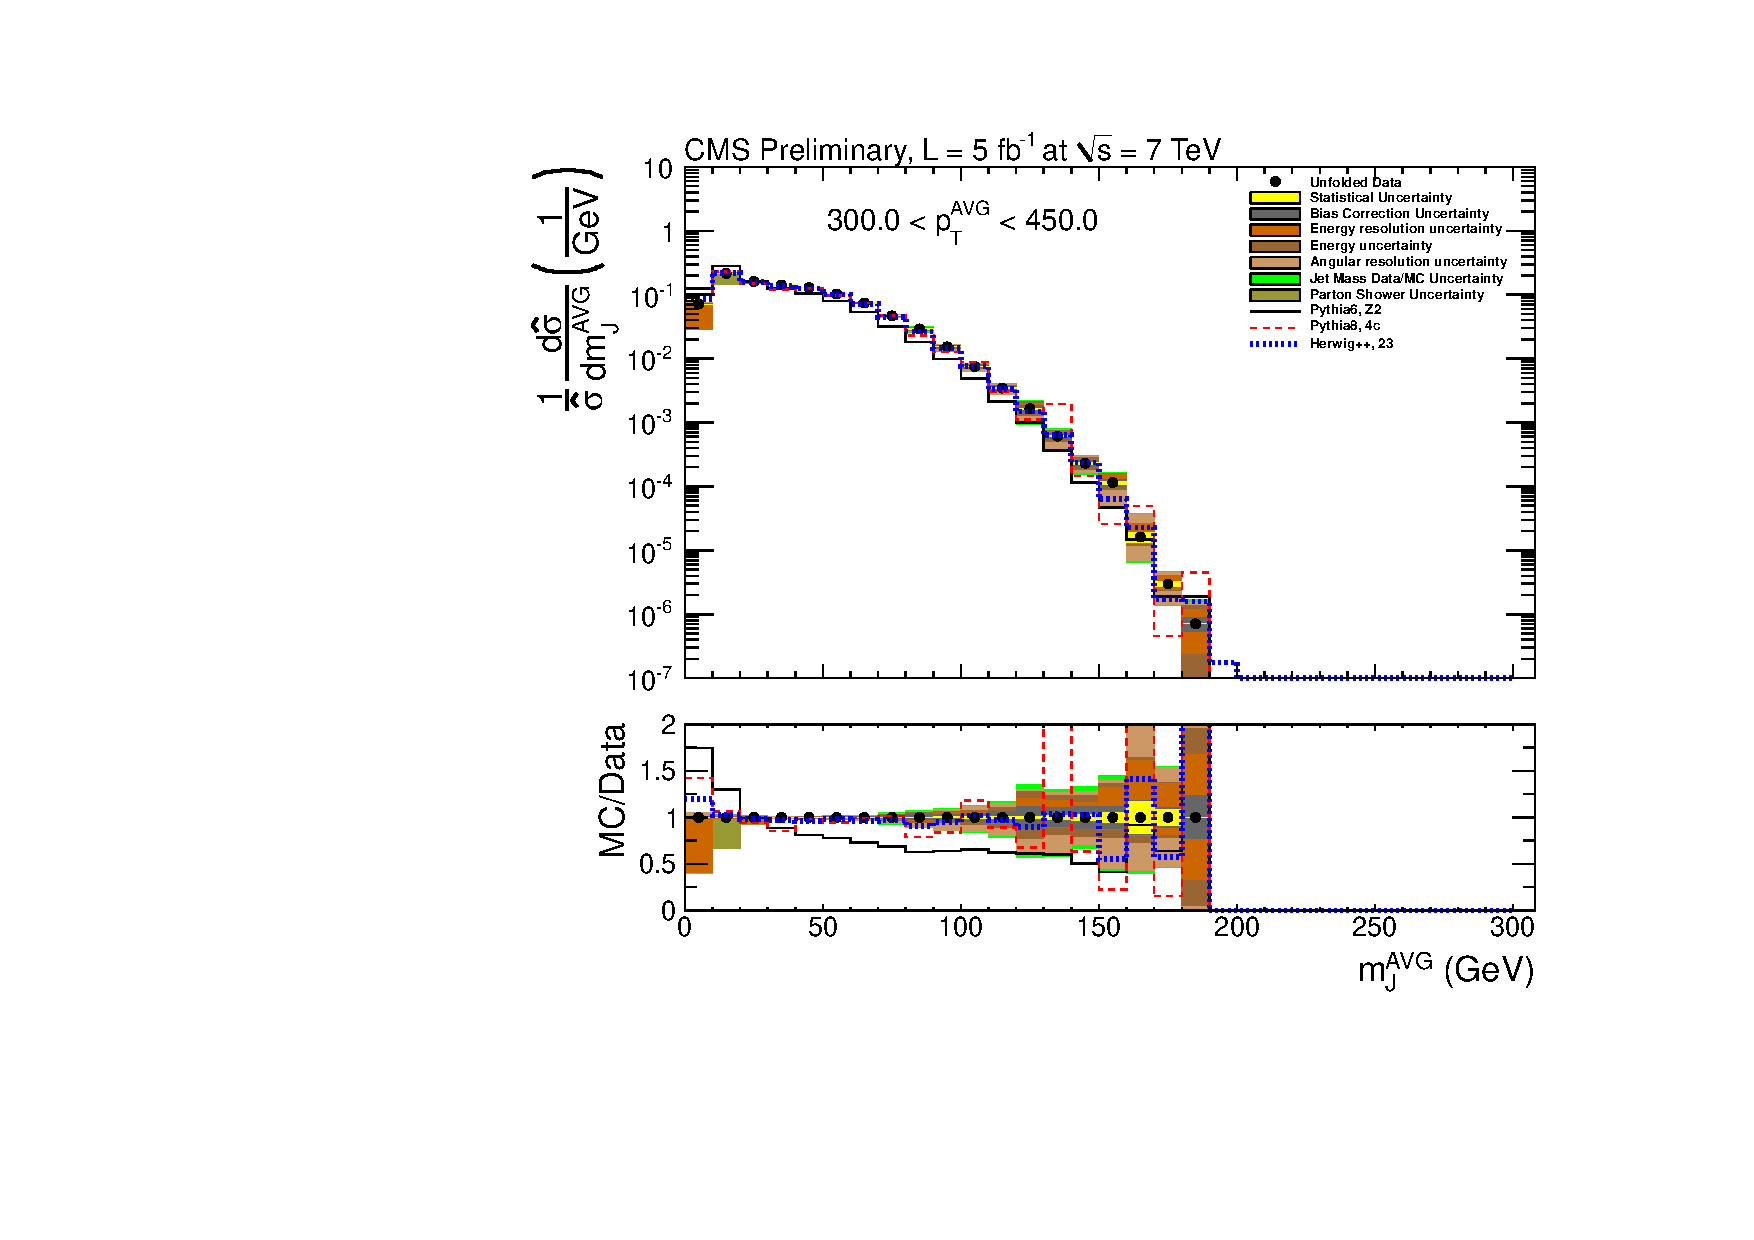
\includegraphics[width=0.95\textwidth]{figs/unfoldedMeasurementDijets_5_Pruned_allsys}
\caption{Unfolded distributions of the jet mass for AK7 Pruned jets,
for $300.0 < \pt^{AVG} < 450.0$ \GeVc. The data are shown in black
points. 
The statistical uncertainty is shown in light yellow, the uncertainties due to the jet-energy resolution, jet-energy scale, and jet-angular resolution are shown in shades of brown, the uncertainty due to pile-up is shown in green, and the uncertainty due to the parton shower are shown in dark yellow.
The simulated distribution from \PYTHIA is shown in solid black, 
the from \PYTHIAEIGHT in dashed red, and from \HERWIG in dotted blue. 
The bottom frame shows the ratio of the true distribution from
the simulation divided by the unfolded distribution, along with
the uncertainties in the unfolded distribution. 
\label{figs:unfoldedMeasurementDijets_5_Pruned_allsys}}
\end{figure}



\begin{figure}[htbp]
\centering
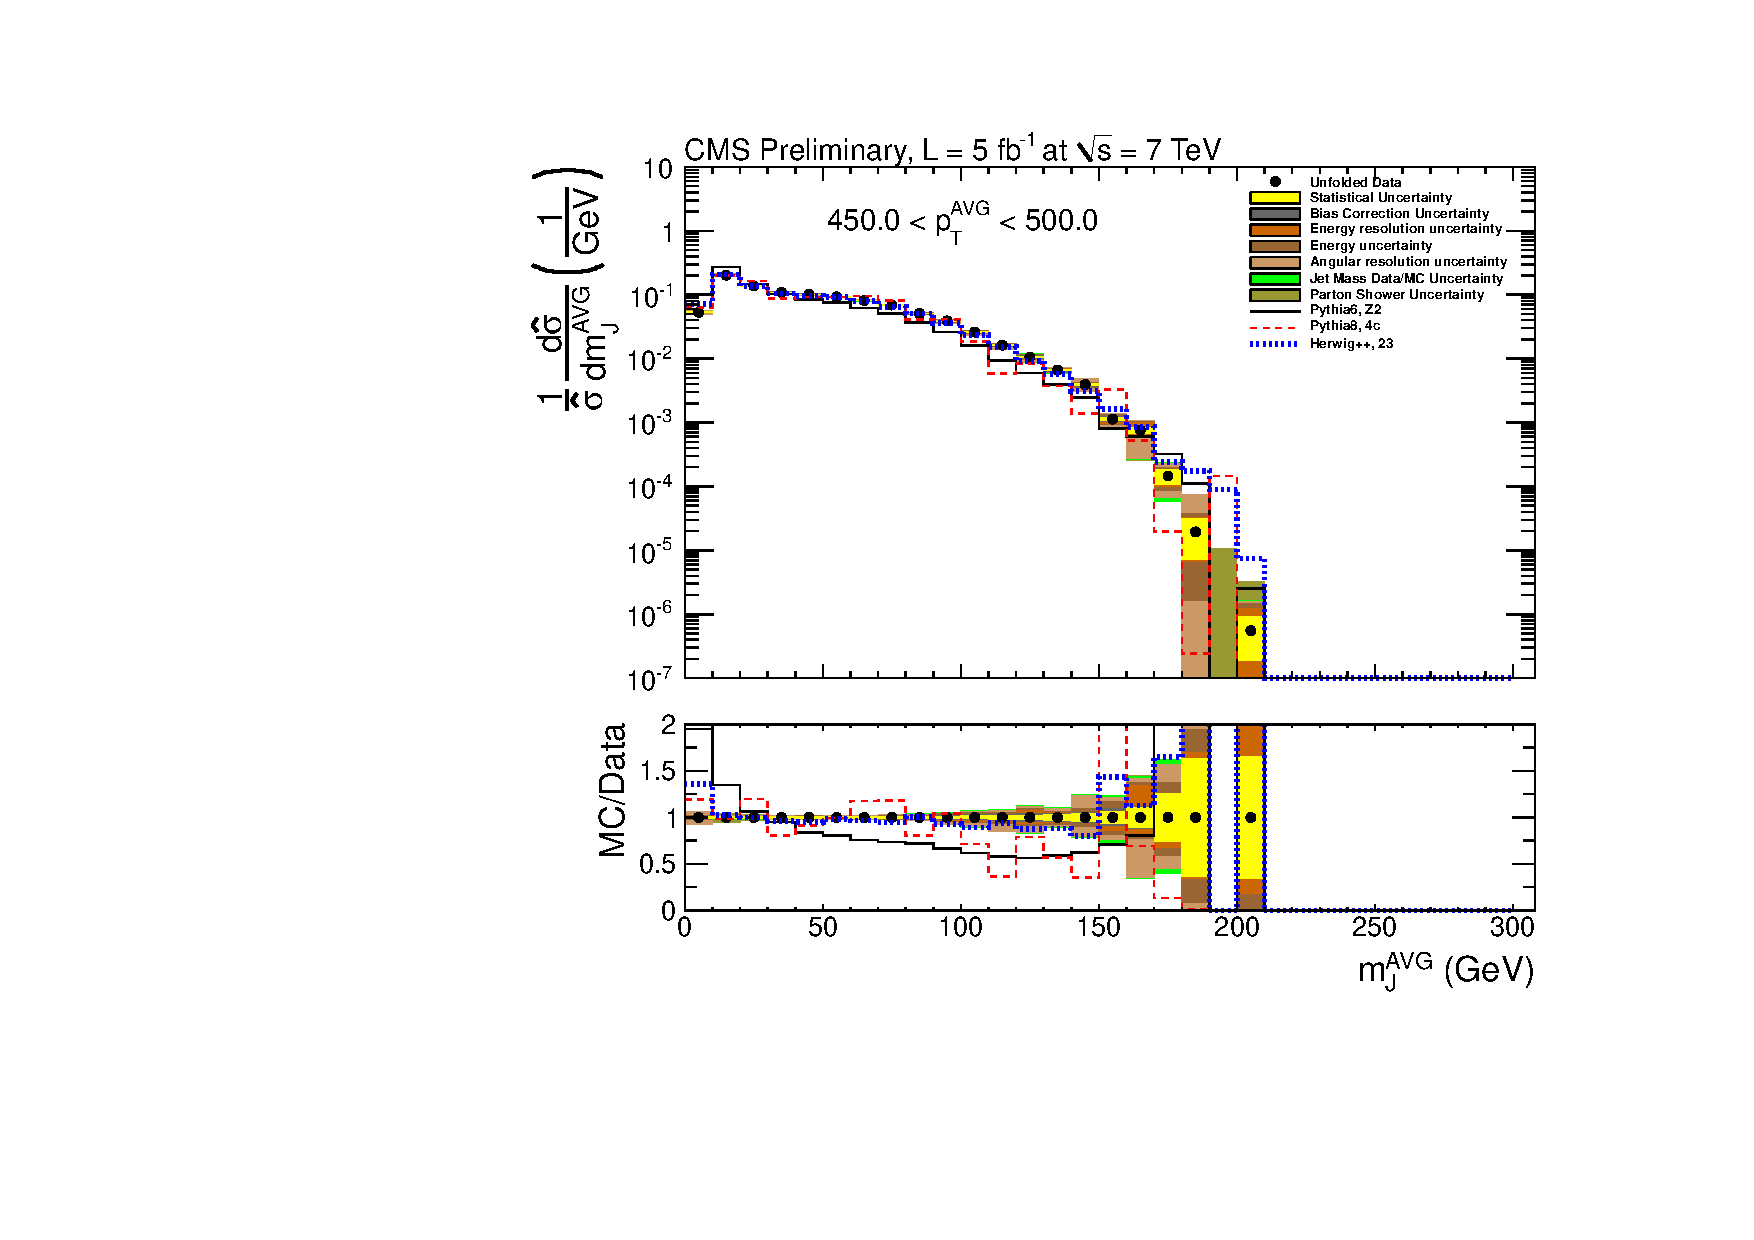
\includegraphics[width=0.95\textwidth]{figs/unfoldedMeasurementDijets_6_Pruned_allsys}
\caption{Unfolded distributions of the jet mass for AK7 Pruned jets,
for $450.0 < \pt^{AVG} < 500.0$ \GeVc. The data are shown in black
points. 
The statistical uncertainty is shown in light yellow, the uncertainties due to the jet-energy resolution, jet-energy scale, and jet-angular resolution are shown in shades of brown, the uncertainty due to pile-up is shown in green, and the uncertainty due to the parton shower are shown in dark yellow.
The simulated distribution from \PYTHIA is shown in solid black, 
the from \PYTHIAEIGHT in dashed red, and from \HERWIG in dotted blue. 
The bottom frame shows the ratio of the true distribution from
the simulation divided by the unfolded distribution, along with
the uncertainties in the unfolded distribution. 
\label{figs:unfoldedMeasurementDijets_6_Pruned_allsys}}
\end{figure}



\begin{figure}[htbp]
\centering
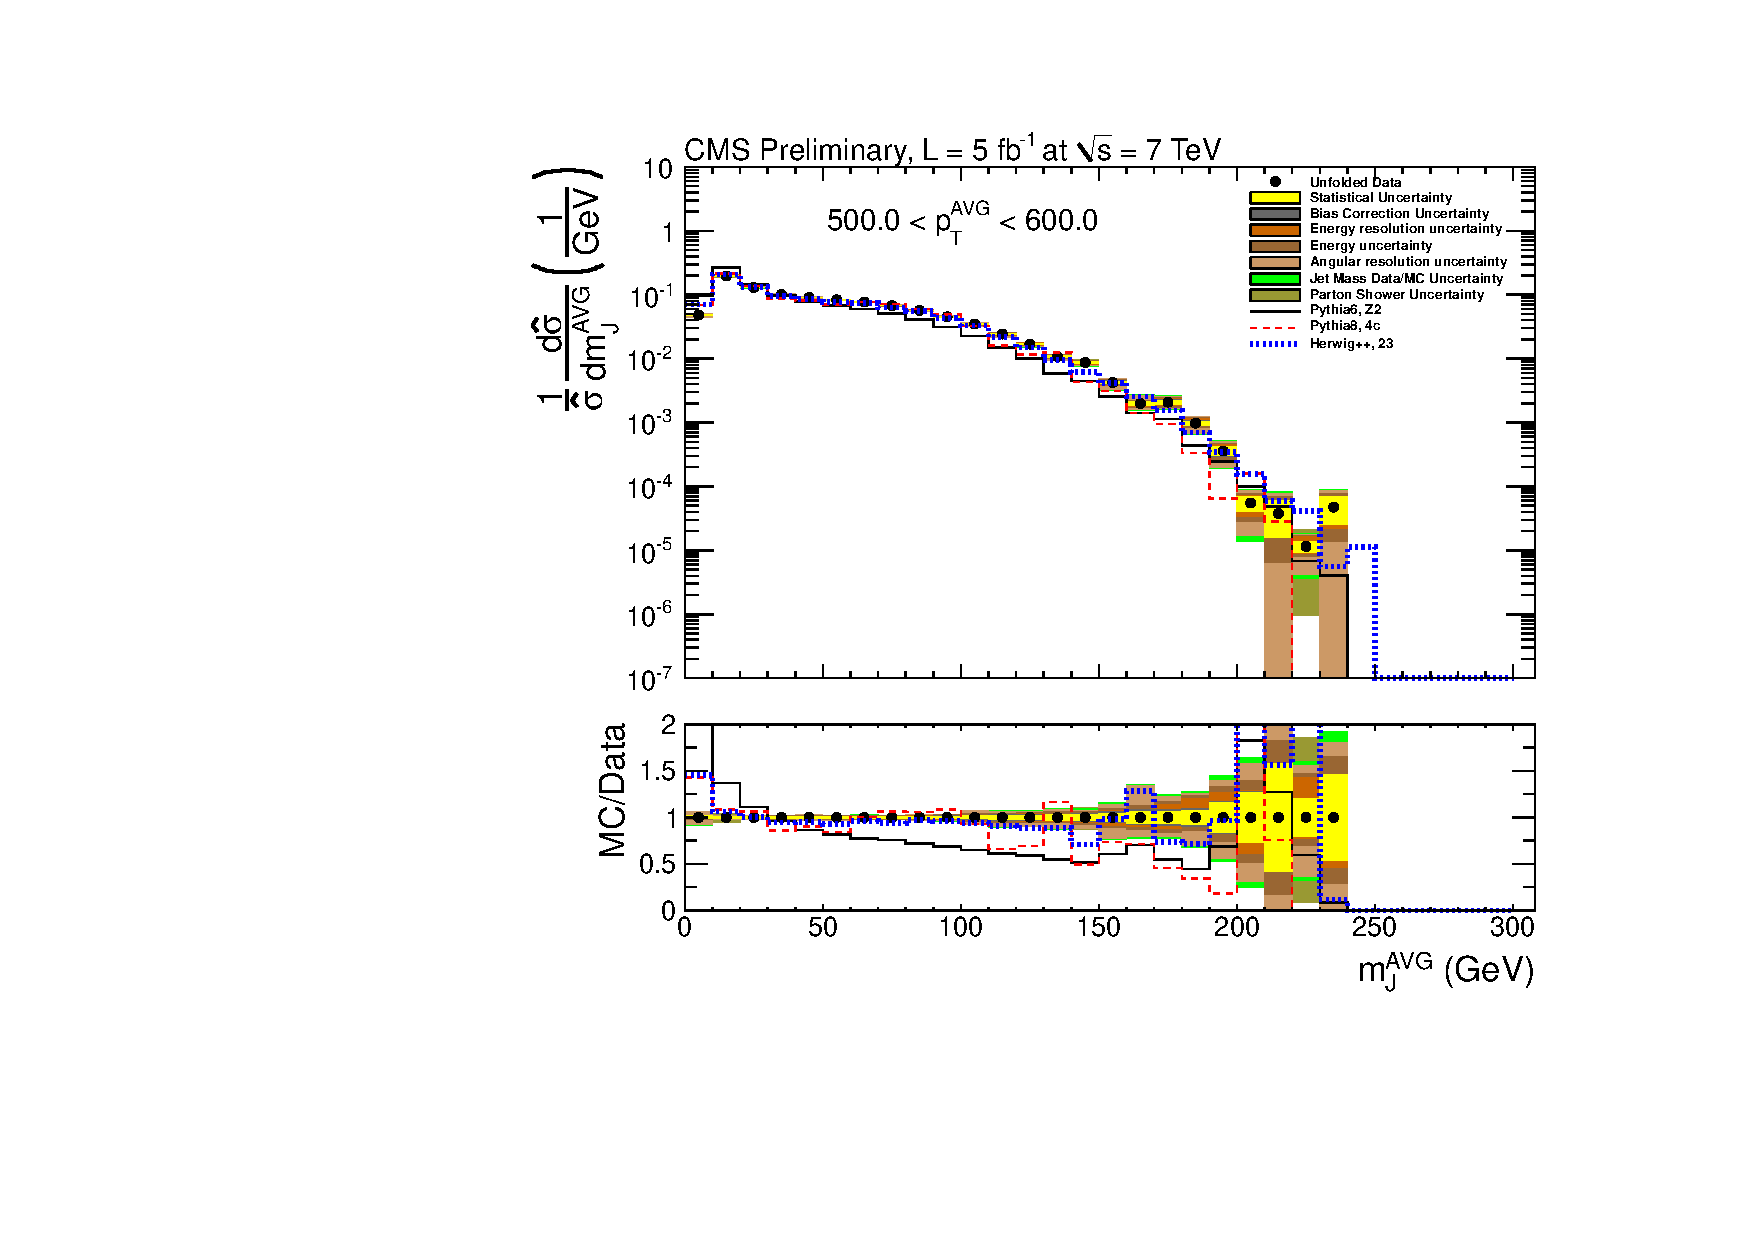
\includegraphics[width=0.95\textwidth]{figs/unfoldedMeasurementDijets_7_Pruned_allsys}
\caption{Unfolded distributions of the jet mass for AK7 Pruned jets,
for $500.0 < \pt^{AVG} < 600.0$ \GeVc. The data are shown in black
points. 
The statistical uncertainty is shown in light yellow, the uncertainties due to the jet-energy resolution, jet-energy scale, and jet-angular resolution are shown in shades of brown, the uncertainty due to pile-up is shown in green, and the uncertainty due to the parton shower are shown in dark yellow.
The simulated distribution from \PYTHIA is shown in solid black, 
the from \PYTHIAEIGHT in dashed red, and from \HERWIG in dotted blue. 
The bottom frame shows the ratio of the true distribution from
the simulation divided by the unfolded distribution, along with
the uncertainties in the unfolded distribution. 
\label{figs:unfoldedMeasurementDijets_7_Pruned_allsys}}
\end{figure}



\begin{figure}[htbp]
\centering
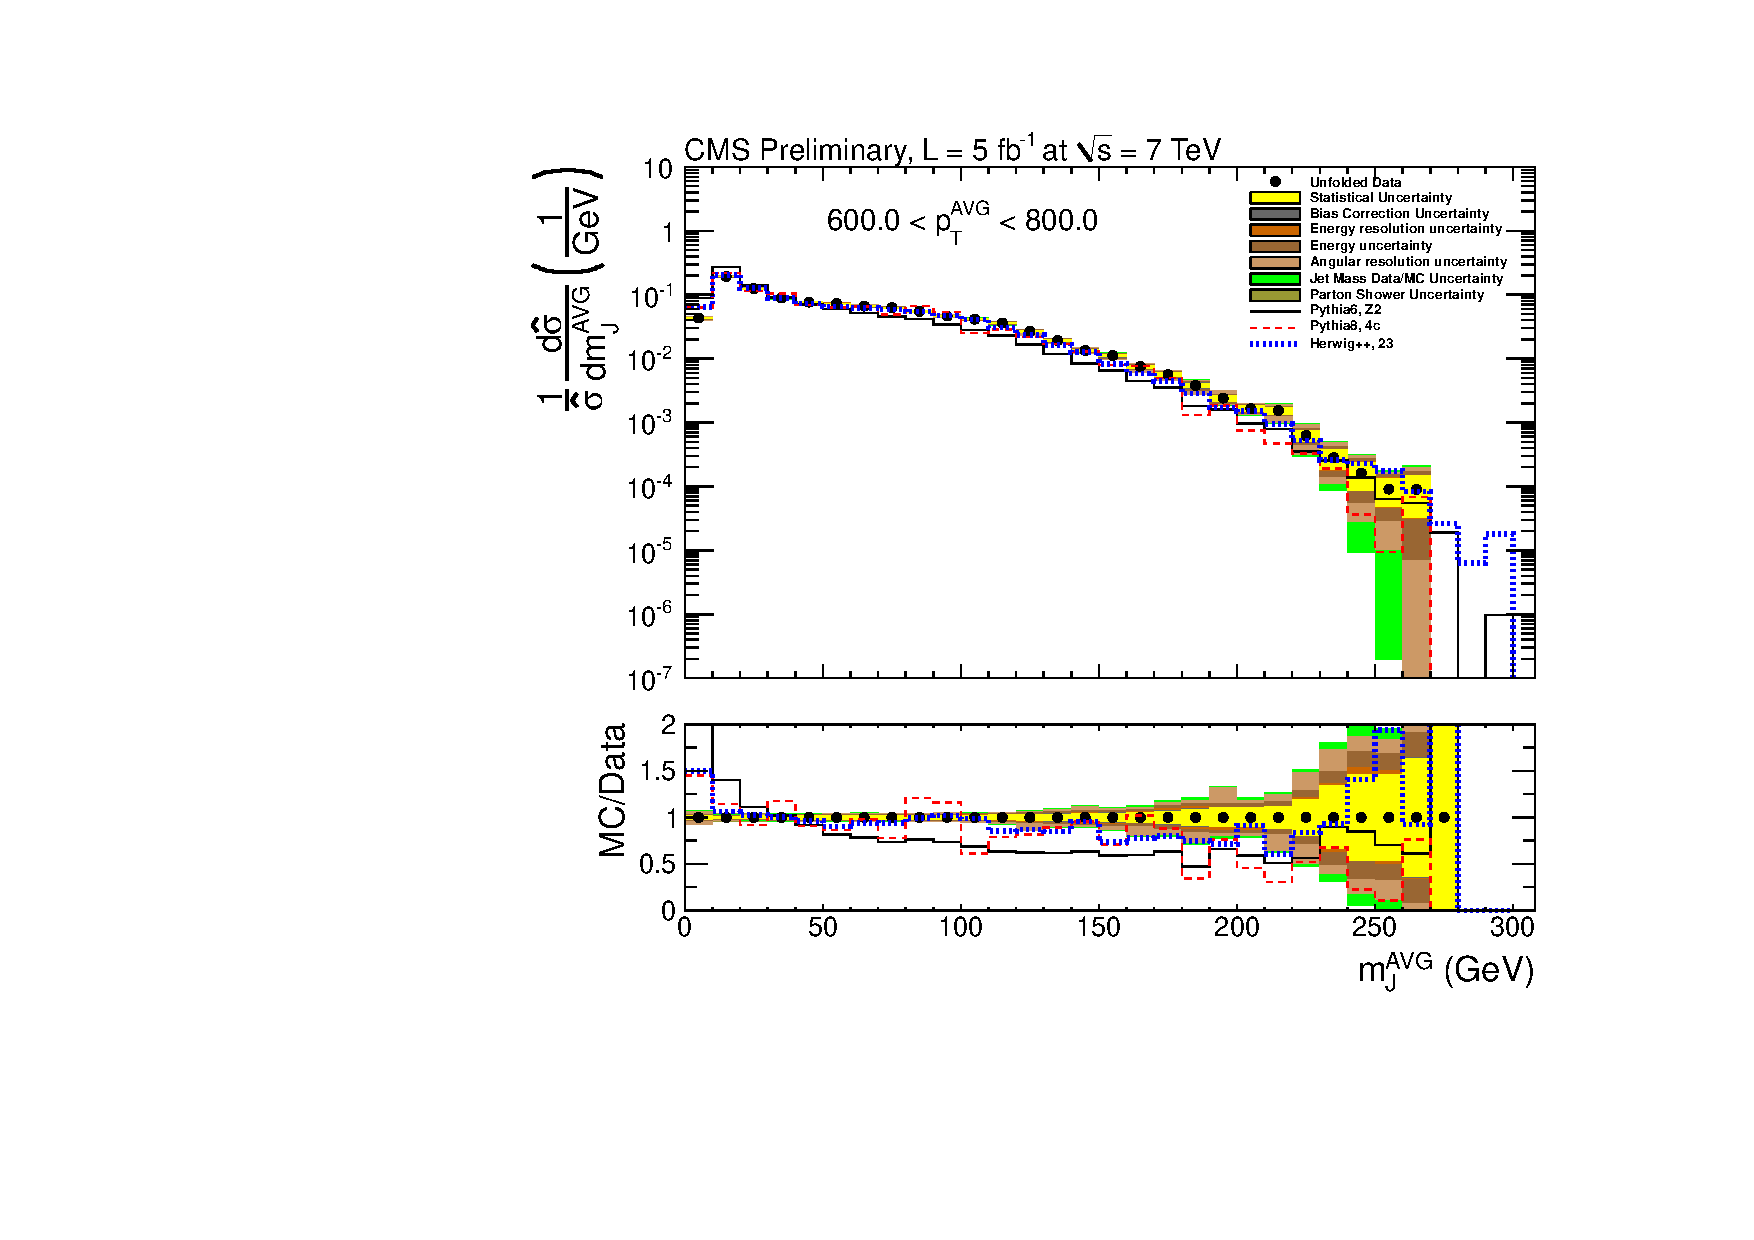
\includegraphics[width=0.95\textwidth]{figs/unfoldedMeasurementDijets_8_Pruned_allsys}
\caption{Unfolded distributions of the jet mass for AK7 Pruned jets,
for $600.0 < \pt^{AVG} < 800.0$ \GeVc. The data are shown in black
points. 
The statistical uncertainty is shown in light yellow, the uncertainties due to the jet-energy resolution, jet-energy scale, and jet-angular resolution are shown in shades of brown, the uncertainty due to pile-up is shown in green, and the uncertainty due to the parton shower are shown in dark yellow.
The simulated distribution from \PYTHIA is shown in solid black, 
the from \PYTHIAEIGHT in dashed red, and from \HERWIG in dotted blue. 
The bottom frame shows the ratio of the true distribution from
the simulation divided by the unfolded distribution, along with
the uncertainties in the unfolded distribution. 
\label{figs:unfoldedMeasurementDijets_8_Pruned_allsys}}
\end{figure}



\begin{figure}[htbp]
\centering
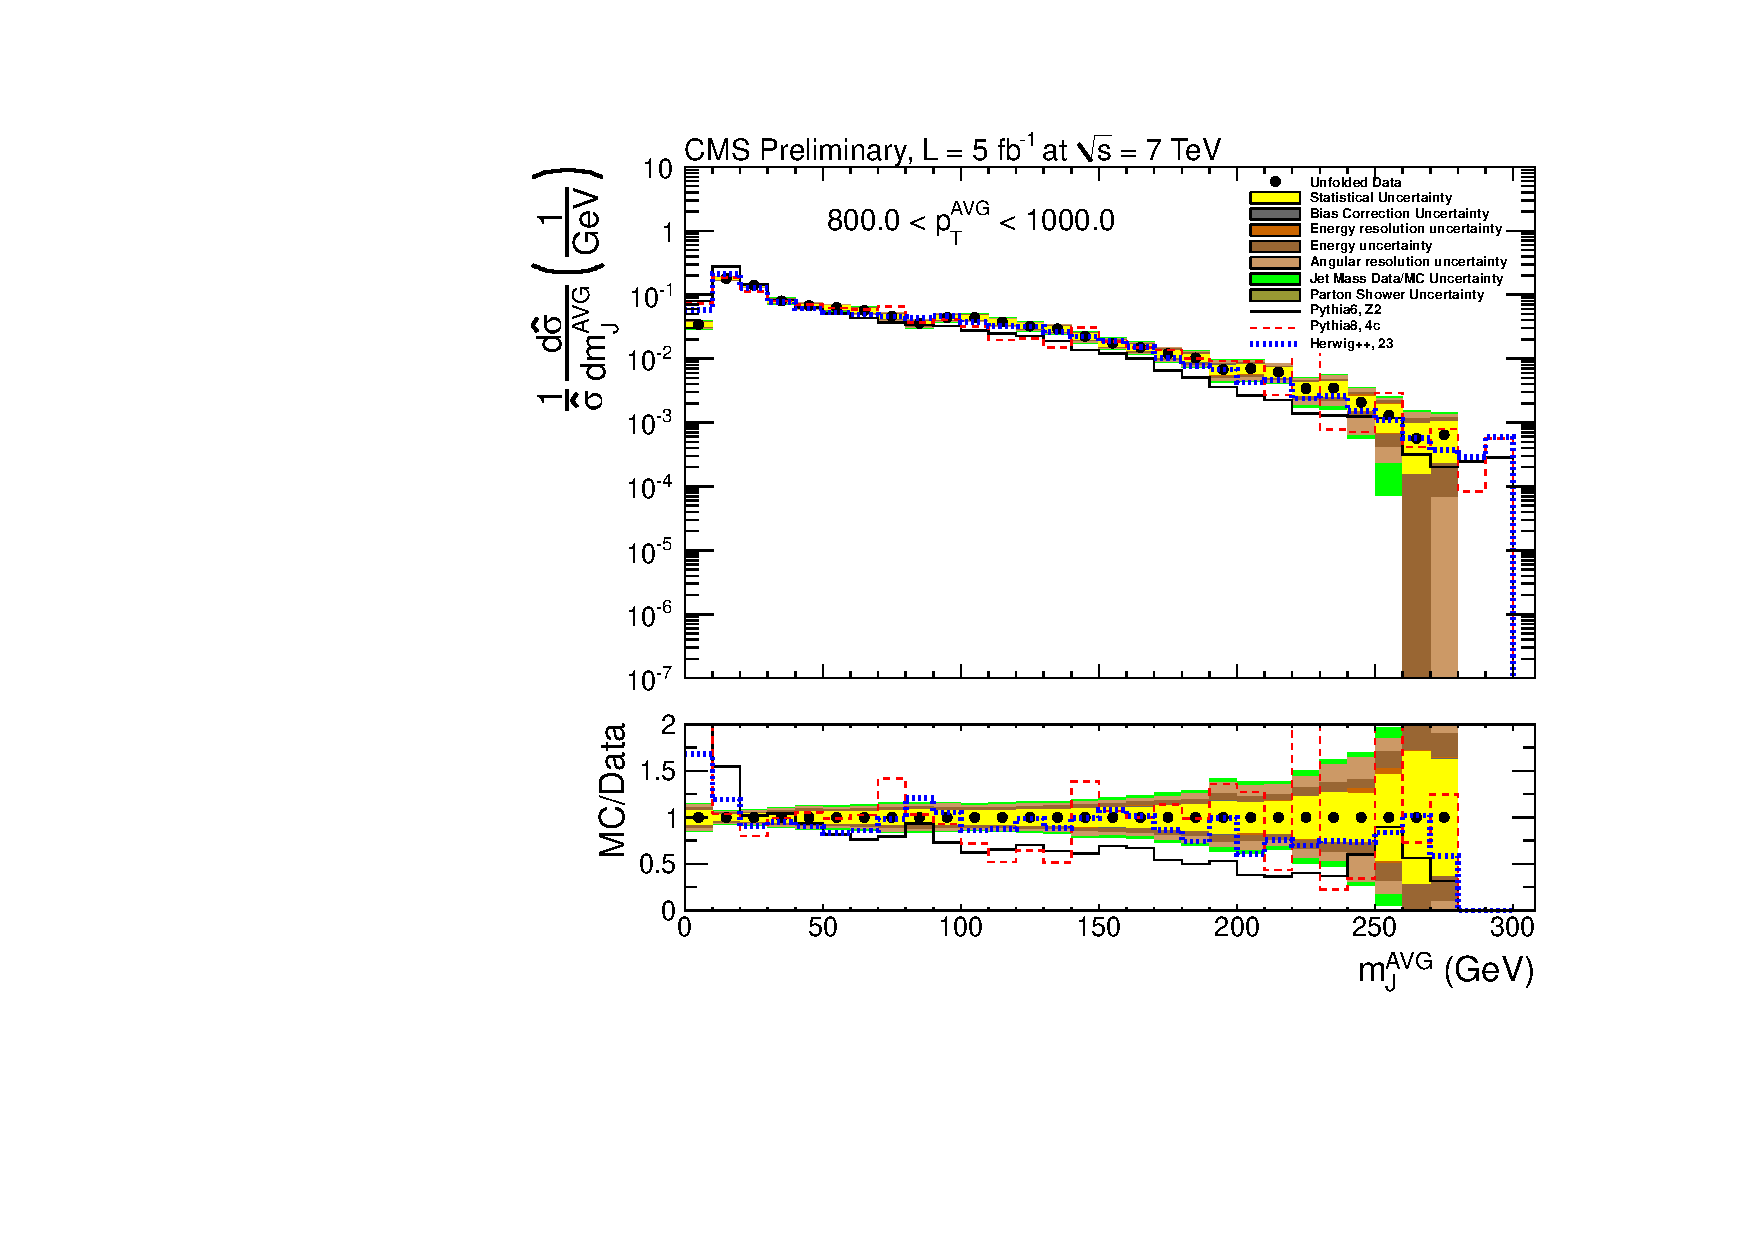
\includegraphics[width=0.95\textwidth]{figs/unfoldedMeasurementDijets_9_Pruned_allsys}
\caption{Unfolded distributions of the jet mass for AK7 Pruned jets,
for $800.0 < \pt^{AVG} < 1000.0$ \GeVc. The data are shown in black
points. 
The statistical uncertainty is shown in light yellow, the uncertainties due to the jet-energy resolution, jet-energy scale, and jet-angular resolution are shown in shades of brown, the uncertainty due to pile-up is shown in green, and the uncertainty due to the parton shower are shown in dark yellow.
The simulated distribution from \PYTHIA is shown in solid black, 
the from \PYTHIAEIGHT in dashed red, and from \HERWIG in dotted blue. 
The bottom frame shows the ratio of the true distribution from
the simulation divided by the unfolded distribution, along with
the uncertainties in the unfolded distribution. 
\label{figs:unfoldedMeasurementDijets_9_Pruned_allsys}}
\end{figure}



\begin{figure}[htbp]
\centering
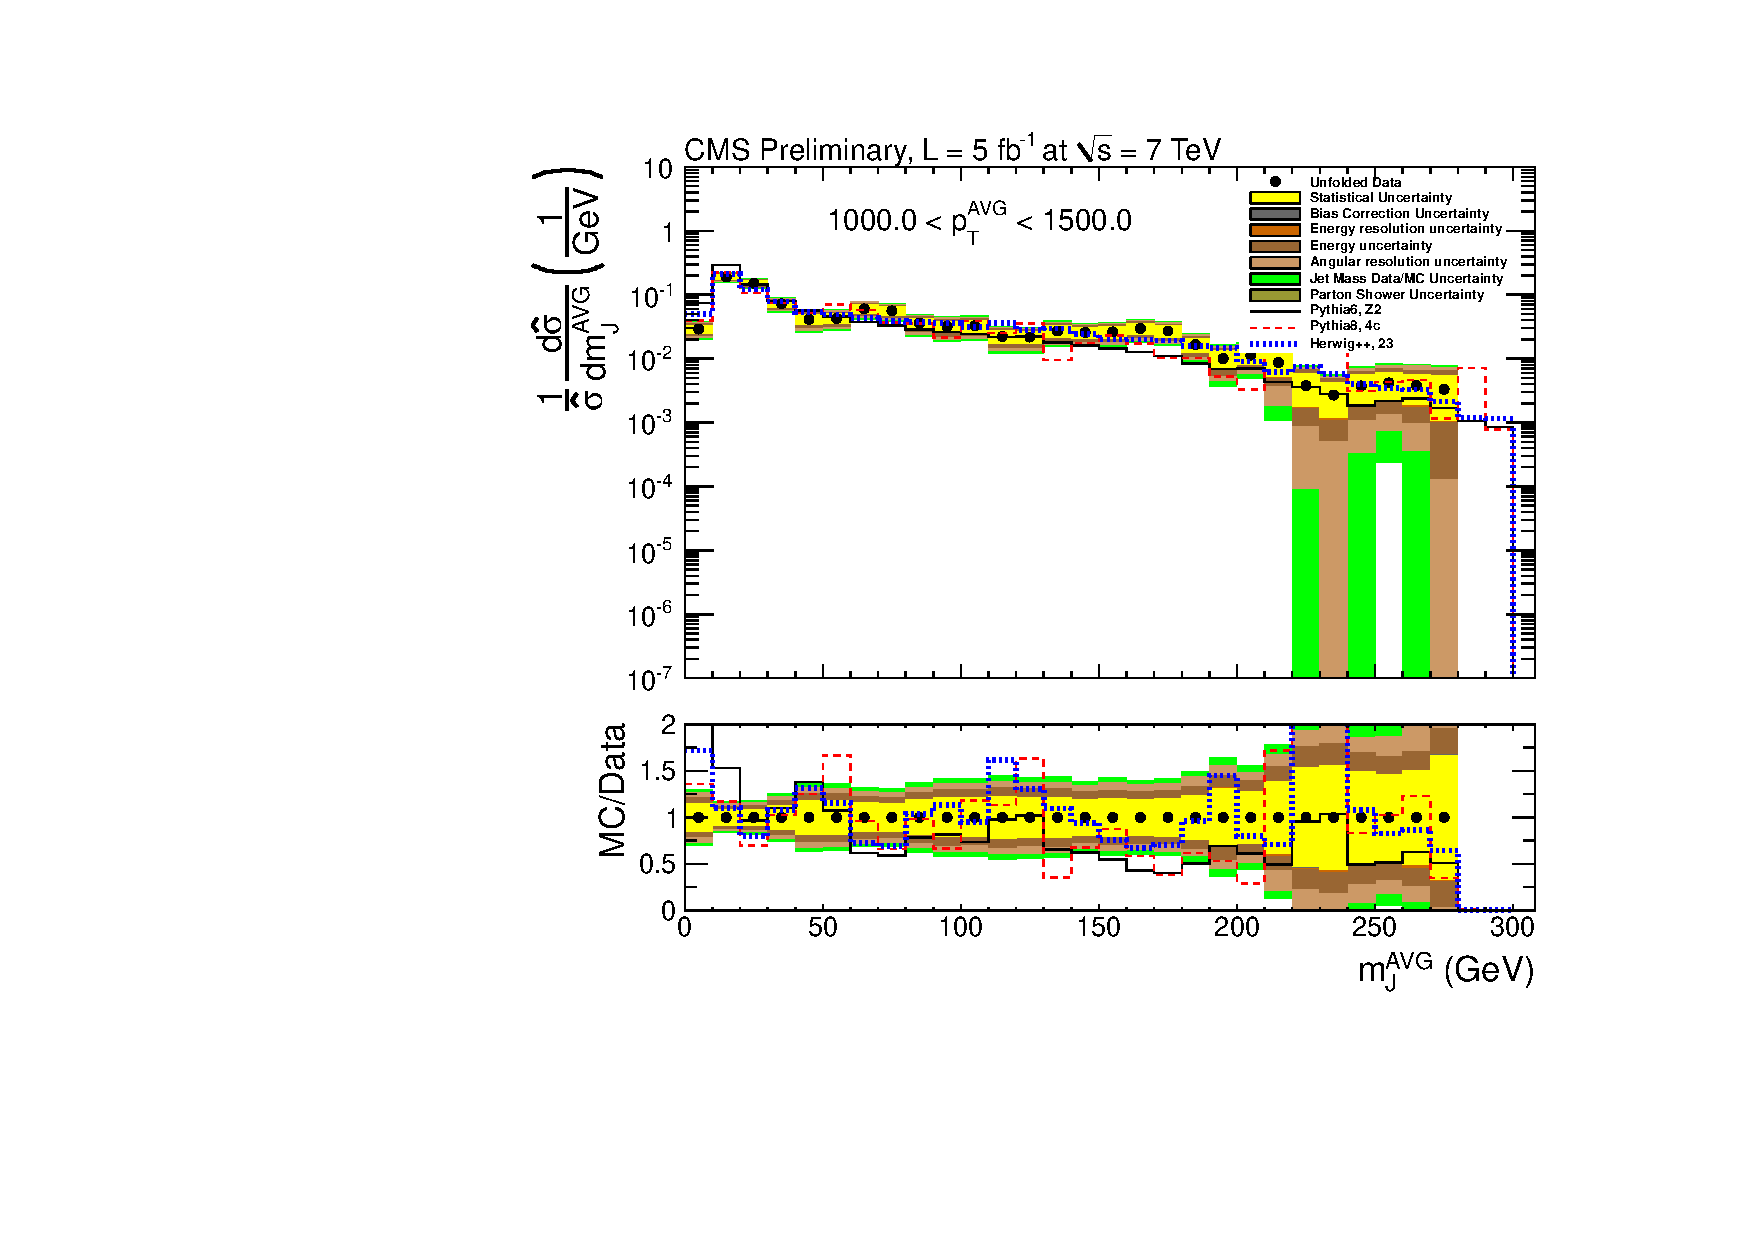
\includegraphics[width=0.95\textwidth]{figs/unfoldedMeasurementDijets_10_Pruned_allsys}
\caption{Unfolded distributions of the jet mass for AK7 Pruned jets,
for $1000.0 < \pt^{AVG} < 1500.0$ \GeVc. The data are shown in black
points. 
The statistical uncertainty is shown in light yellow, the uncertainties due to the jet-energy resolution, jet-energy scale, and jet-angular resolution are shown in shades of brown, the uncertainty due to pile-up is shown in green, and the uncertainty due to the parton shower are shown in dark yellow.
The simulated distribution from \PYTHIA is shown in solid black, 
the from \PYTHIAEIGHT in dashed red, and from \HERWIG in dotted blue. 
The bottom frame shows the ratio of the true distribution from
the simulation divided by the unfolded distribution, along with
the uncertainties in the unfolded distribution. 
\label{figs:unfoldedMeasurementDijets_10_Pruned_allsys}}
\end{figure}

\clearpage

\fi


\ifnpas

\begin{figure}[htbp]
\centering
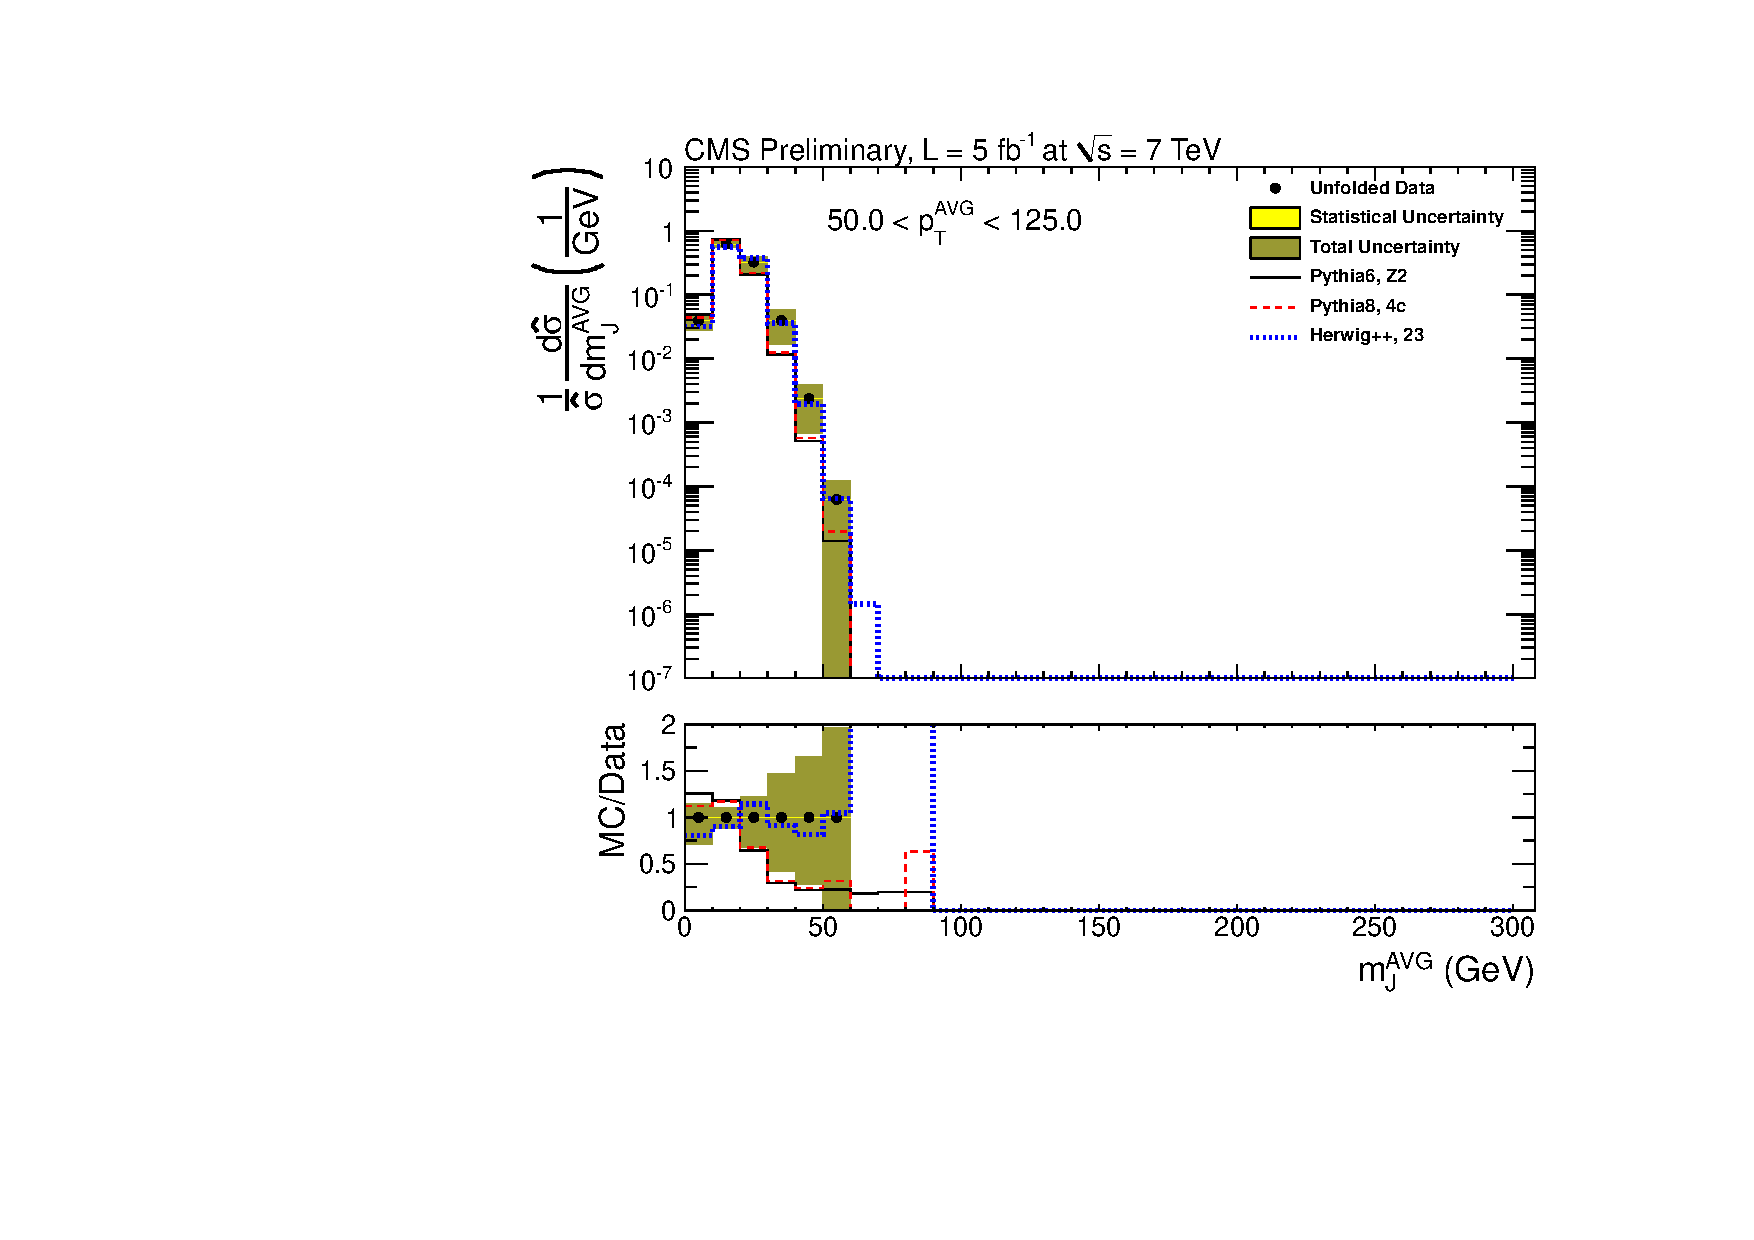
\includegraphics[width=0.95\textwidth]{figs/unfoldedMeasurementDijets_1}
\caption{Unfolded distributions of the jet mass for AK7 jets,
for $50.0 < \pt^{AVG} < 125.0$ \GeVc. The data are shown in black
points. 
The statistical uncertainty is shown in light yellow (light gray), and the statistical plus systematic uncertainty is shown in dark yellow (dark gray).
The simulated distribution from \PYTHIA is shown in solid black, 
the from \PYTHIAEIGHT in dashed red, and from \HERWIG in dotted blue. 
The bottom frame shows the ratio of the true distribution from
the simulation divided by the unfolded distribution, along with
the uncertainties in the unfolded distribution. 
\label{figs:unfoldedMeasurementDijets_1}}
\end{figure}

\fi

\begin{figure}[htbp]
\centering
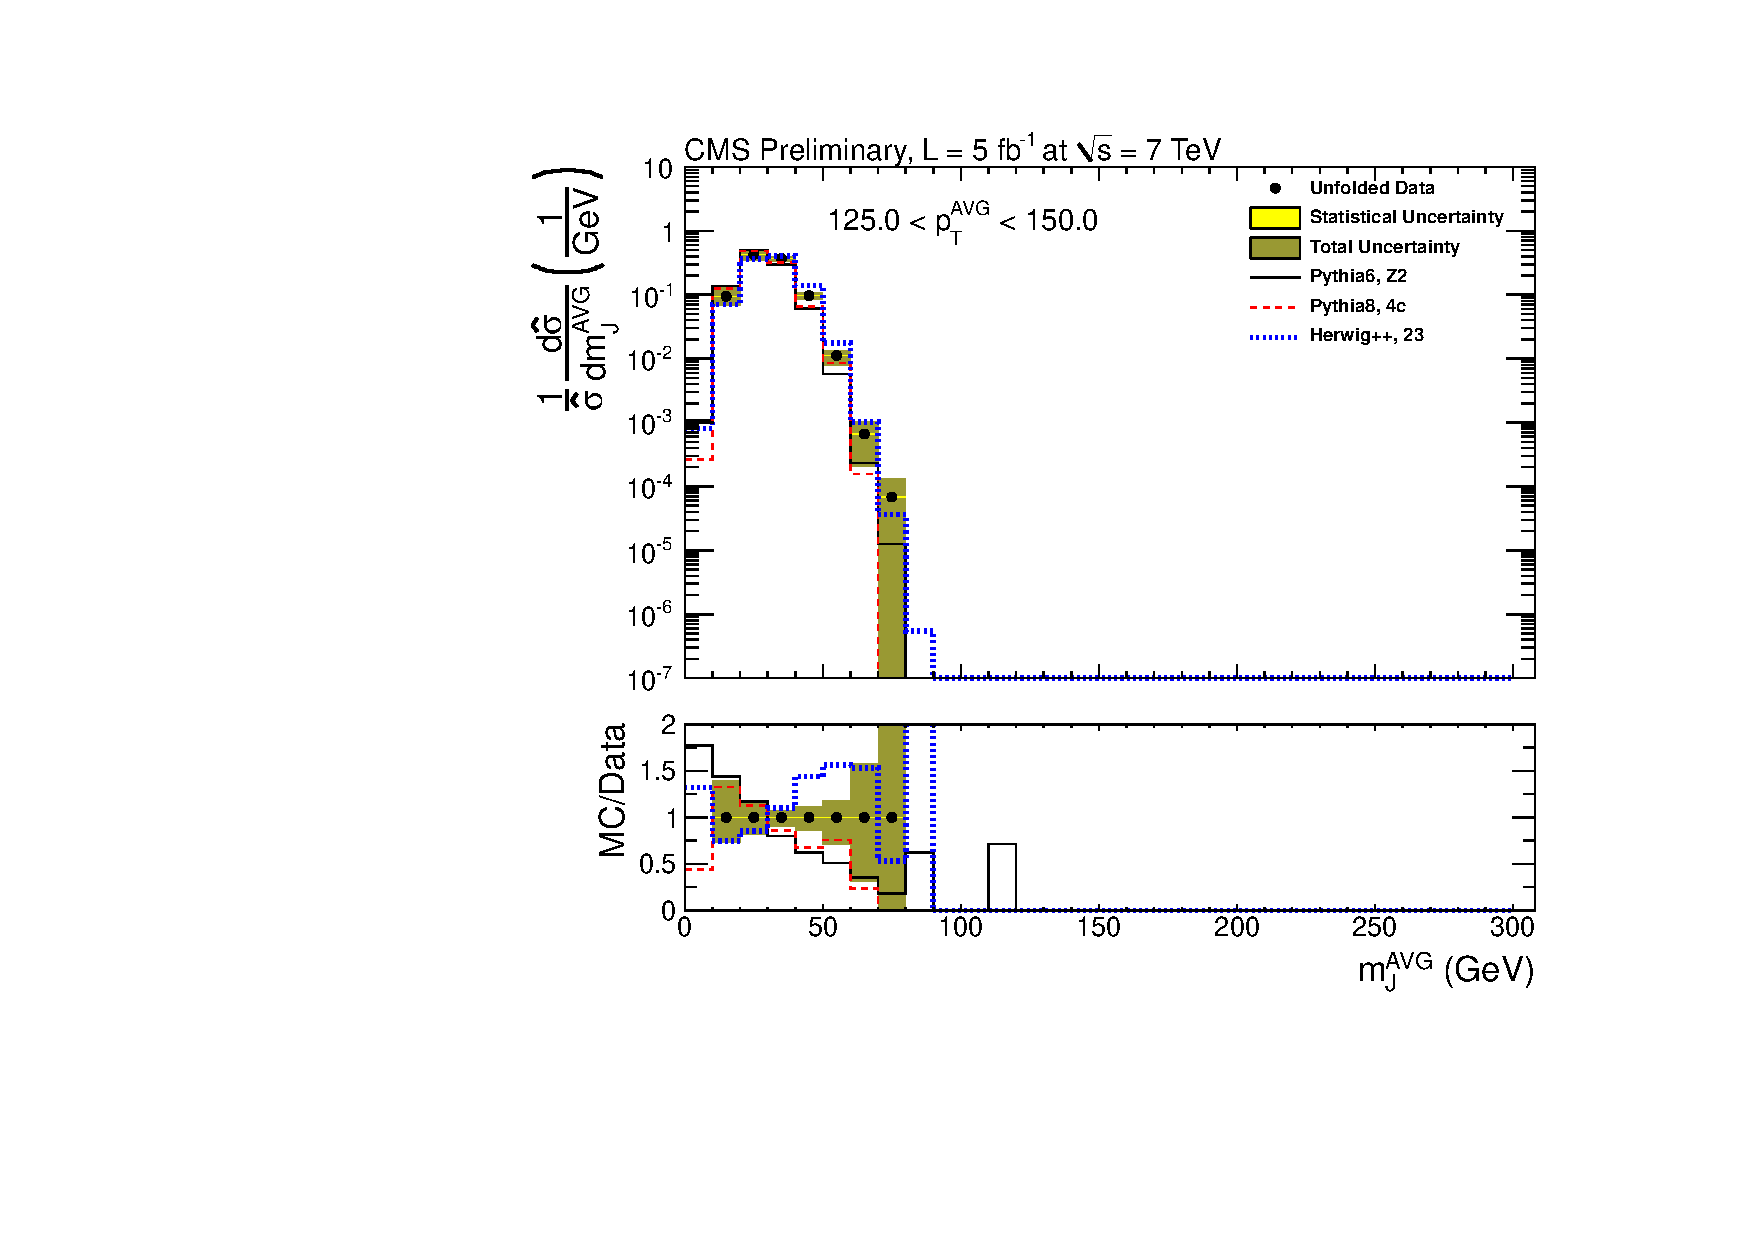
\includegraphics[width=0.49\textwidth]{figs/unfoldedMeasurementDijets_2}
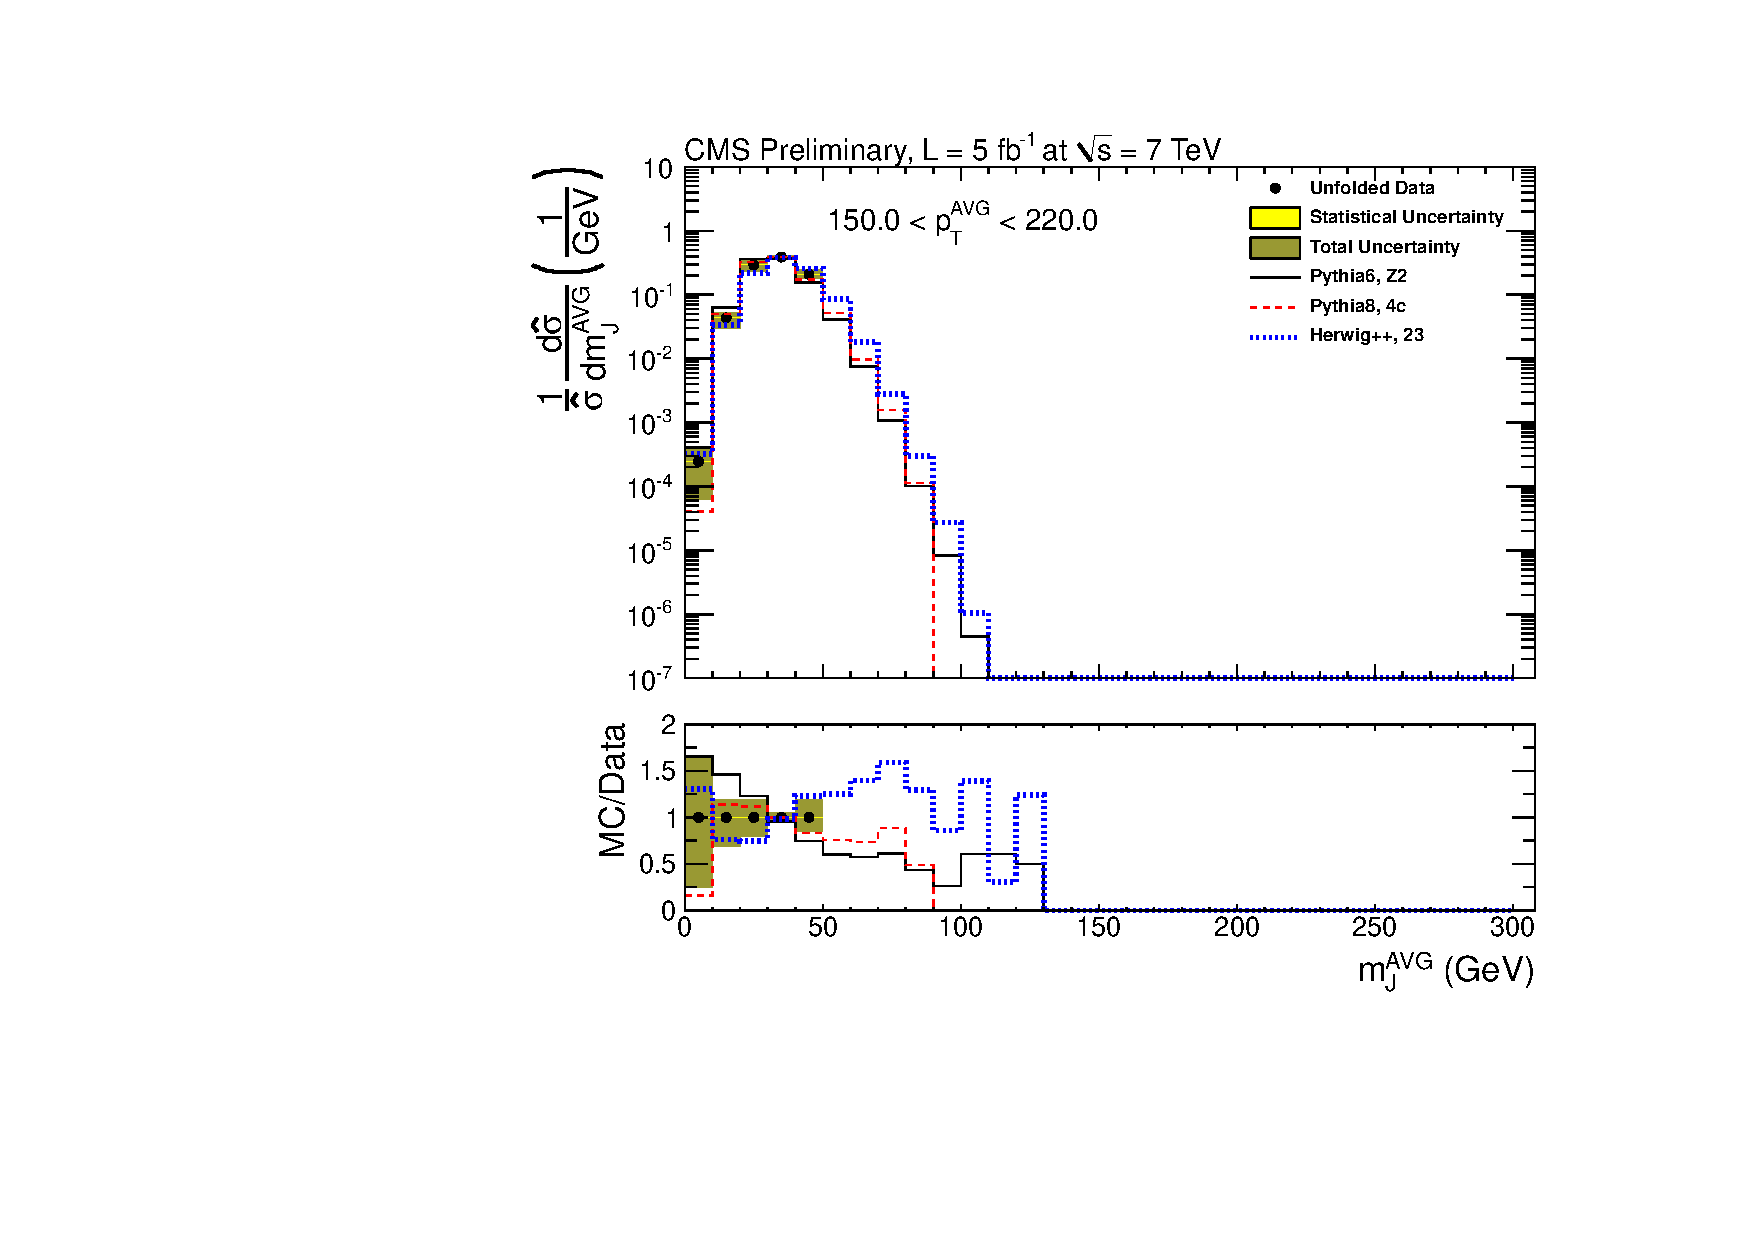
\includegraphics[width=0.49\textwidth]{figs/unfoldedMeasurementDijets_3}
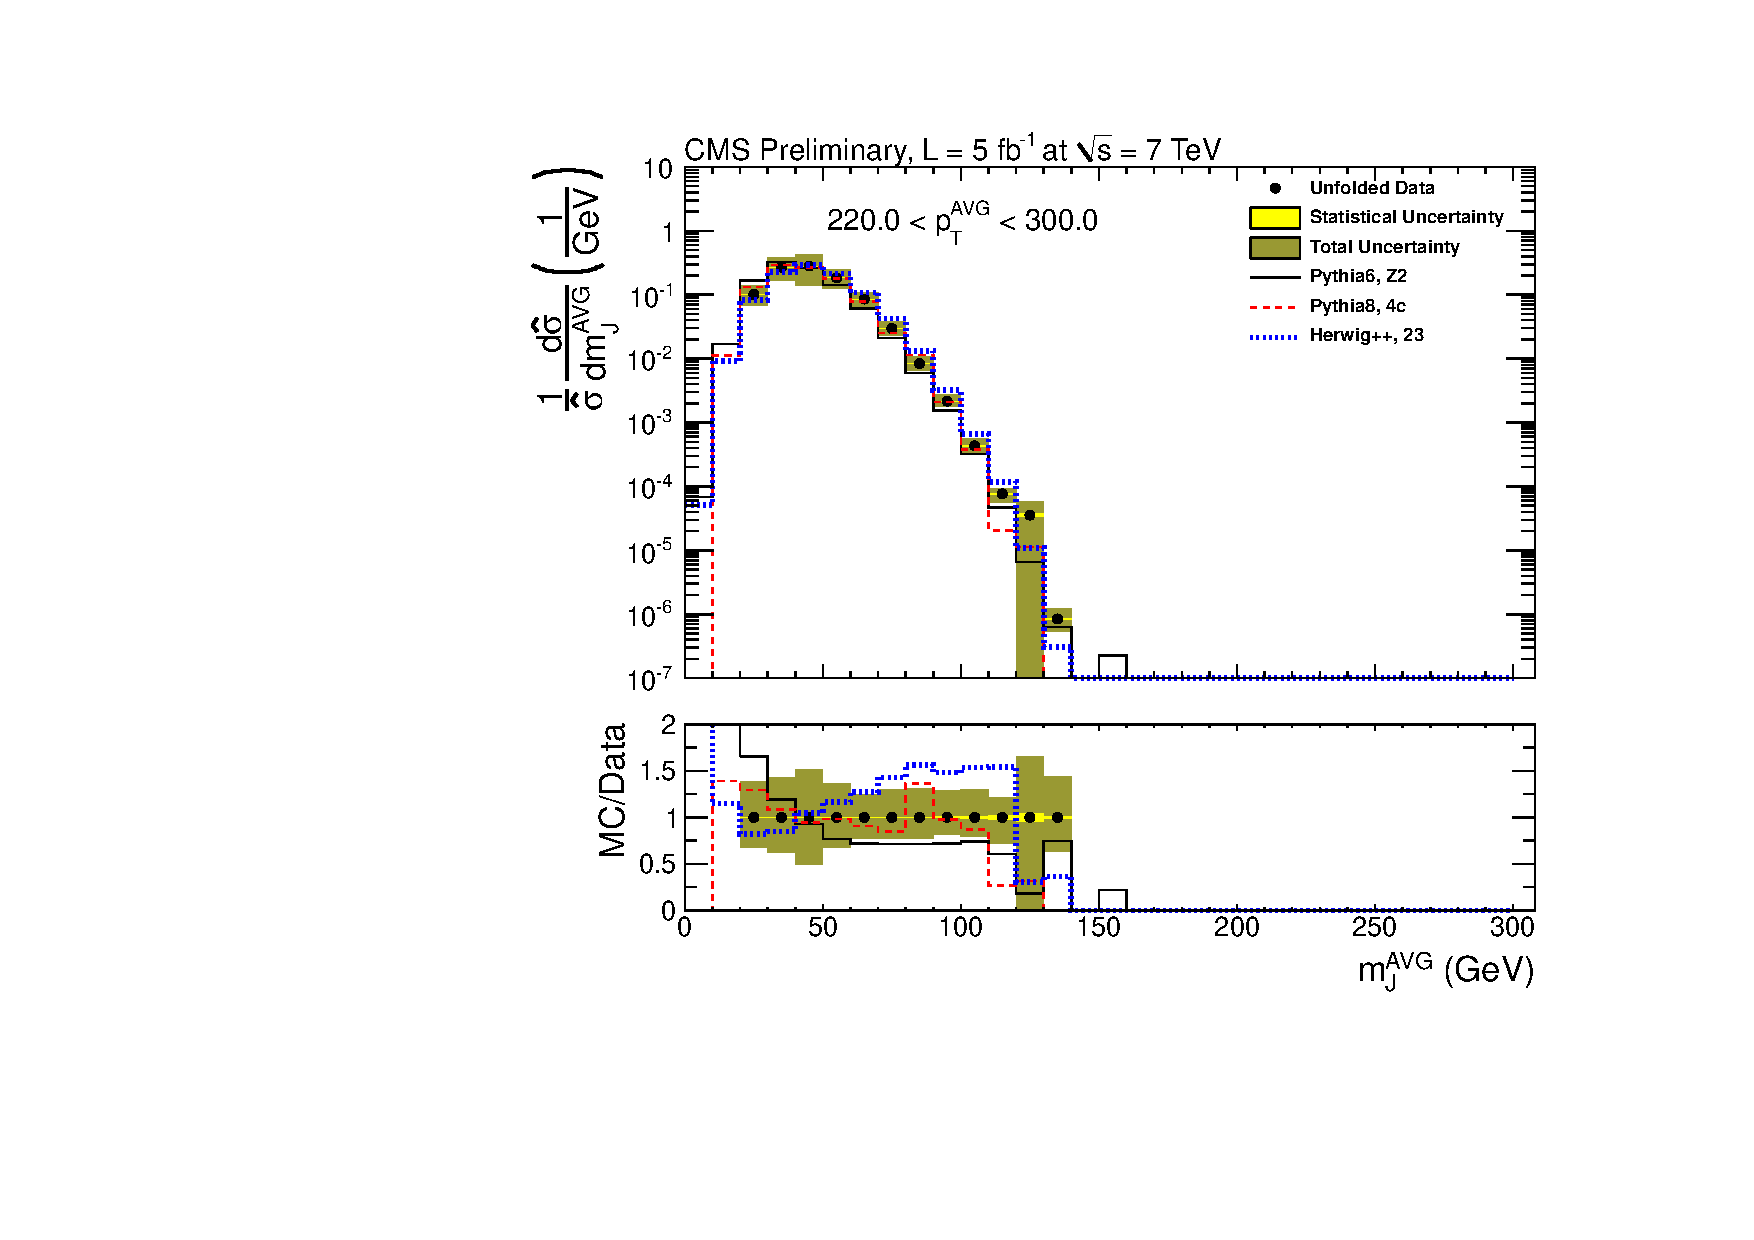
\includegraphics[width=0.49\textwidth]{figs/unfoldedMeasurementDijets_4}
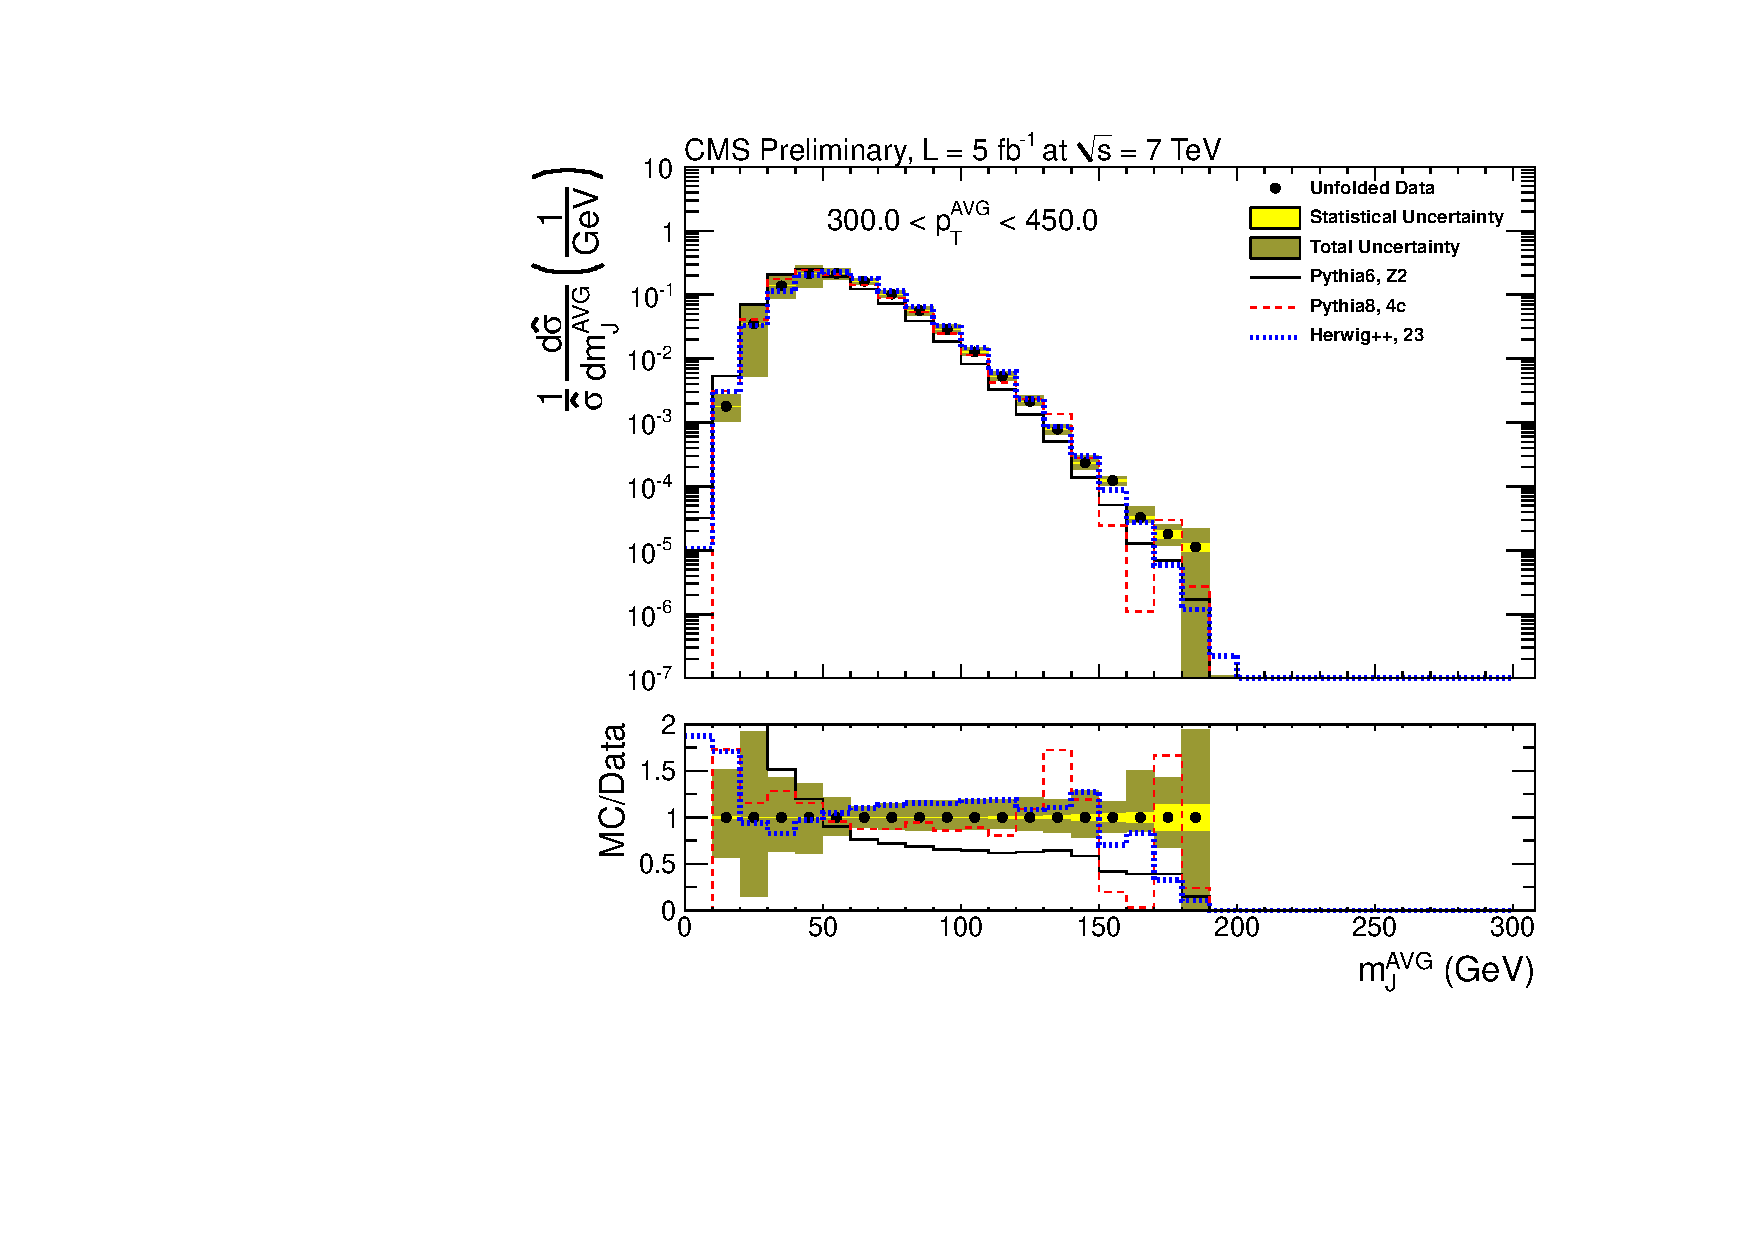
\includegraphics[width=0.49\textwidth]{figs/unfoldedMeasurementDijets_5}
\caption{Unfolded distributions of the jet mass for AK7 jets,
%for $125.0 < \pt^{AVG} < 150.0$ \GeVc. The data are shown in black
for several $\pt^{AVG}$ bins. The data are shown in black
points. 
The statistical uncertainty is shown in light yellow (light gray), and the statistical plus systematic uncertainty is shown in dark yellow (dark gray).
The simulated distribution from \PYTHIA is shown in solid black, 
the from \PYTHIAEIGHT in dashed red, and from \HERWIG in dotted blue. 
The bottom frame shows the ratio of the true distribution from
the simulation divided by the unfolded distribution, along with
the uncertainties in the unfolded distribution. 
\label{figs:unfoldedMeasurementDijets_2}}
\end{figure}

%%%%
\ifnpas

\begin{figure}[htbp]
\centering
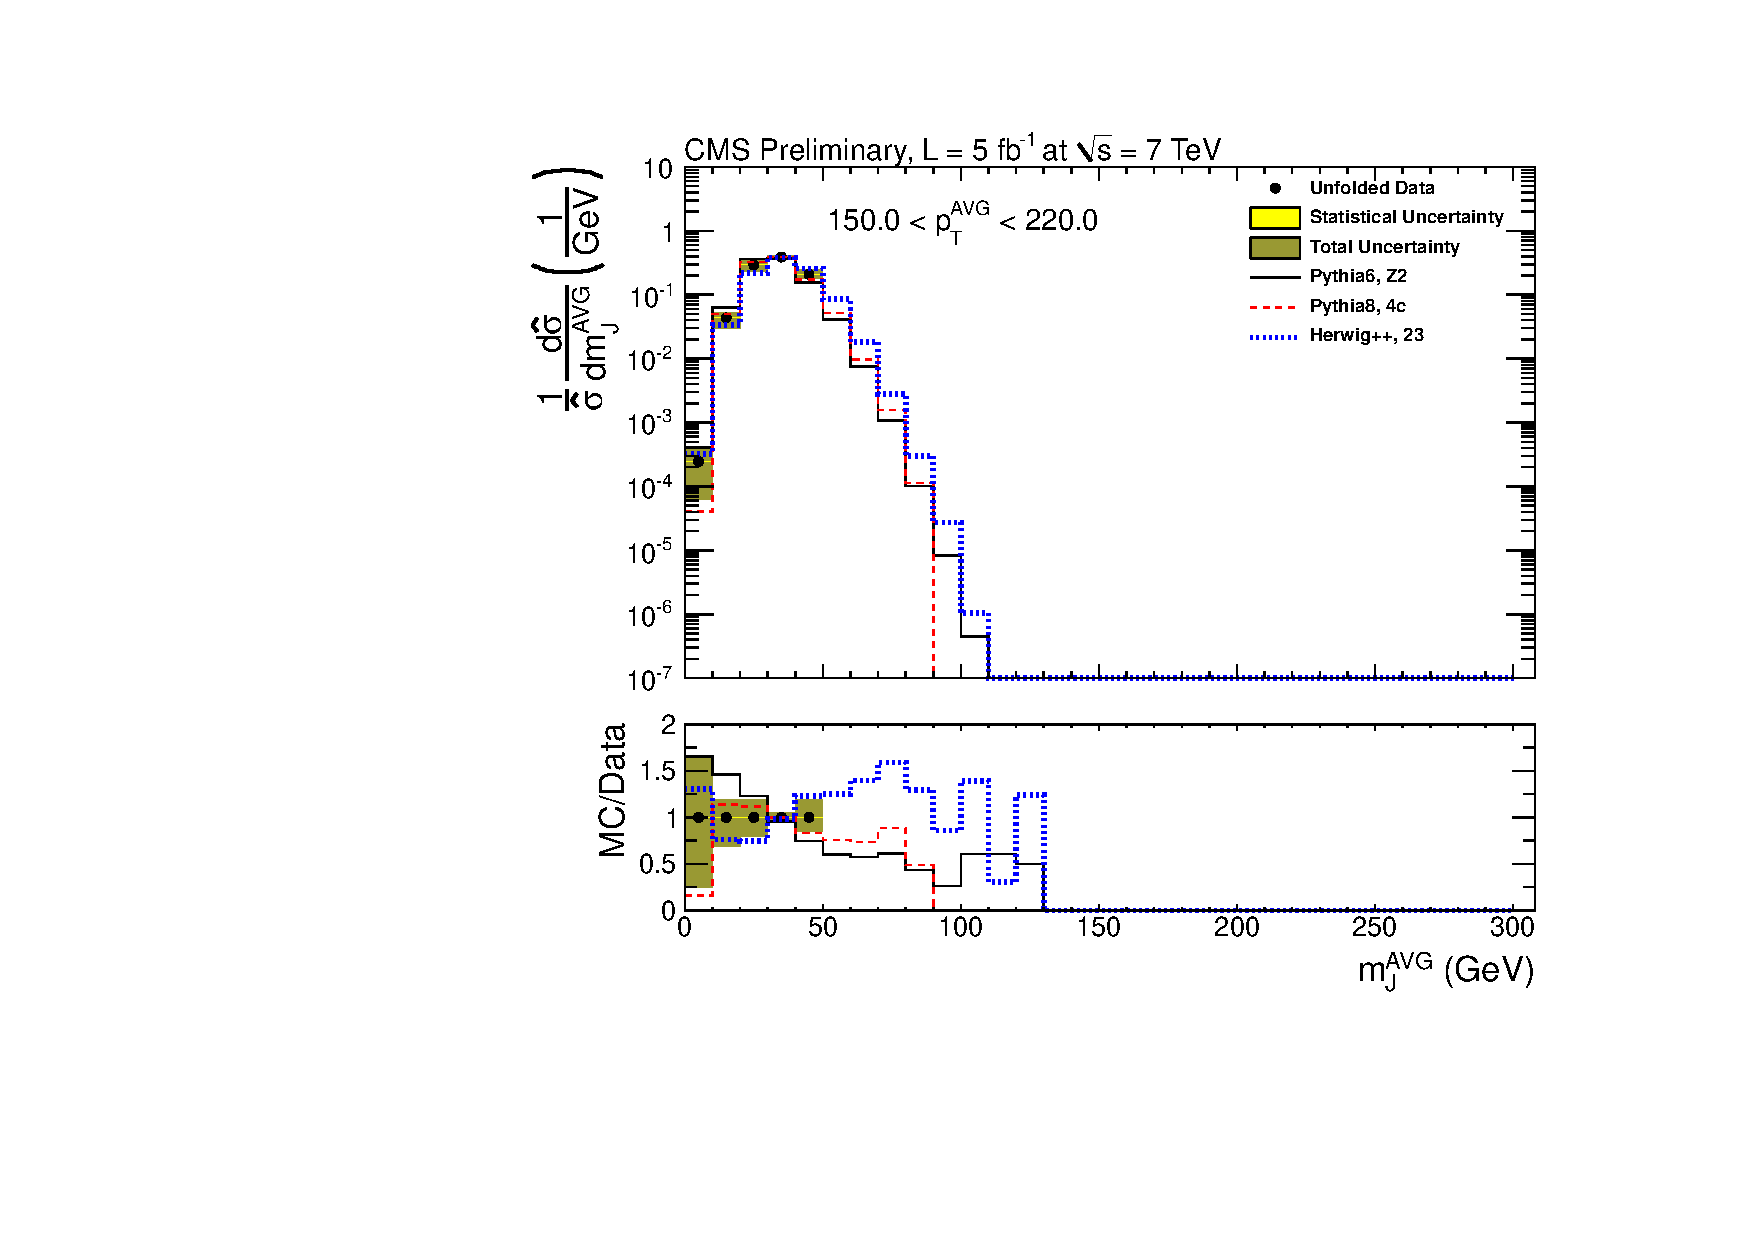
\includegraphics[width=0.95\textwidth]{figs/unfoldedMeasurementDijets_3}
\caption{Unfolded distributions of the jet mass for AK7 jets,
for $150.0 < \pt^{AVG} < 220.0$ \GeVc. The data are shown in black
points. 
The statistical uncertainty is shown in light yellow (light gray), and the statistical plus systematic uncertainty is shown in dark yellow (dark gray).
The simulated distribution from \PYTHIA is shown in solid black, 
the from \PYTHIAEIGHT in dashed red, and from \HERWIG in dotted blue. 
The bottom frame shows the ratio of the true distribution from
the simulation divided by the unfolded distribution, along with
the uncertainties in the unfolded distribution. 
\label{figs:unfoldedMeasurementDijets_3}}
\end{figure}



\begin{figure}[htbp]
\centering
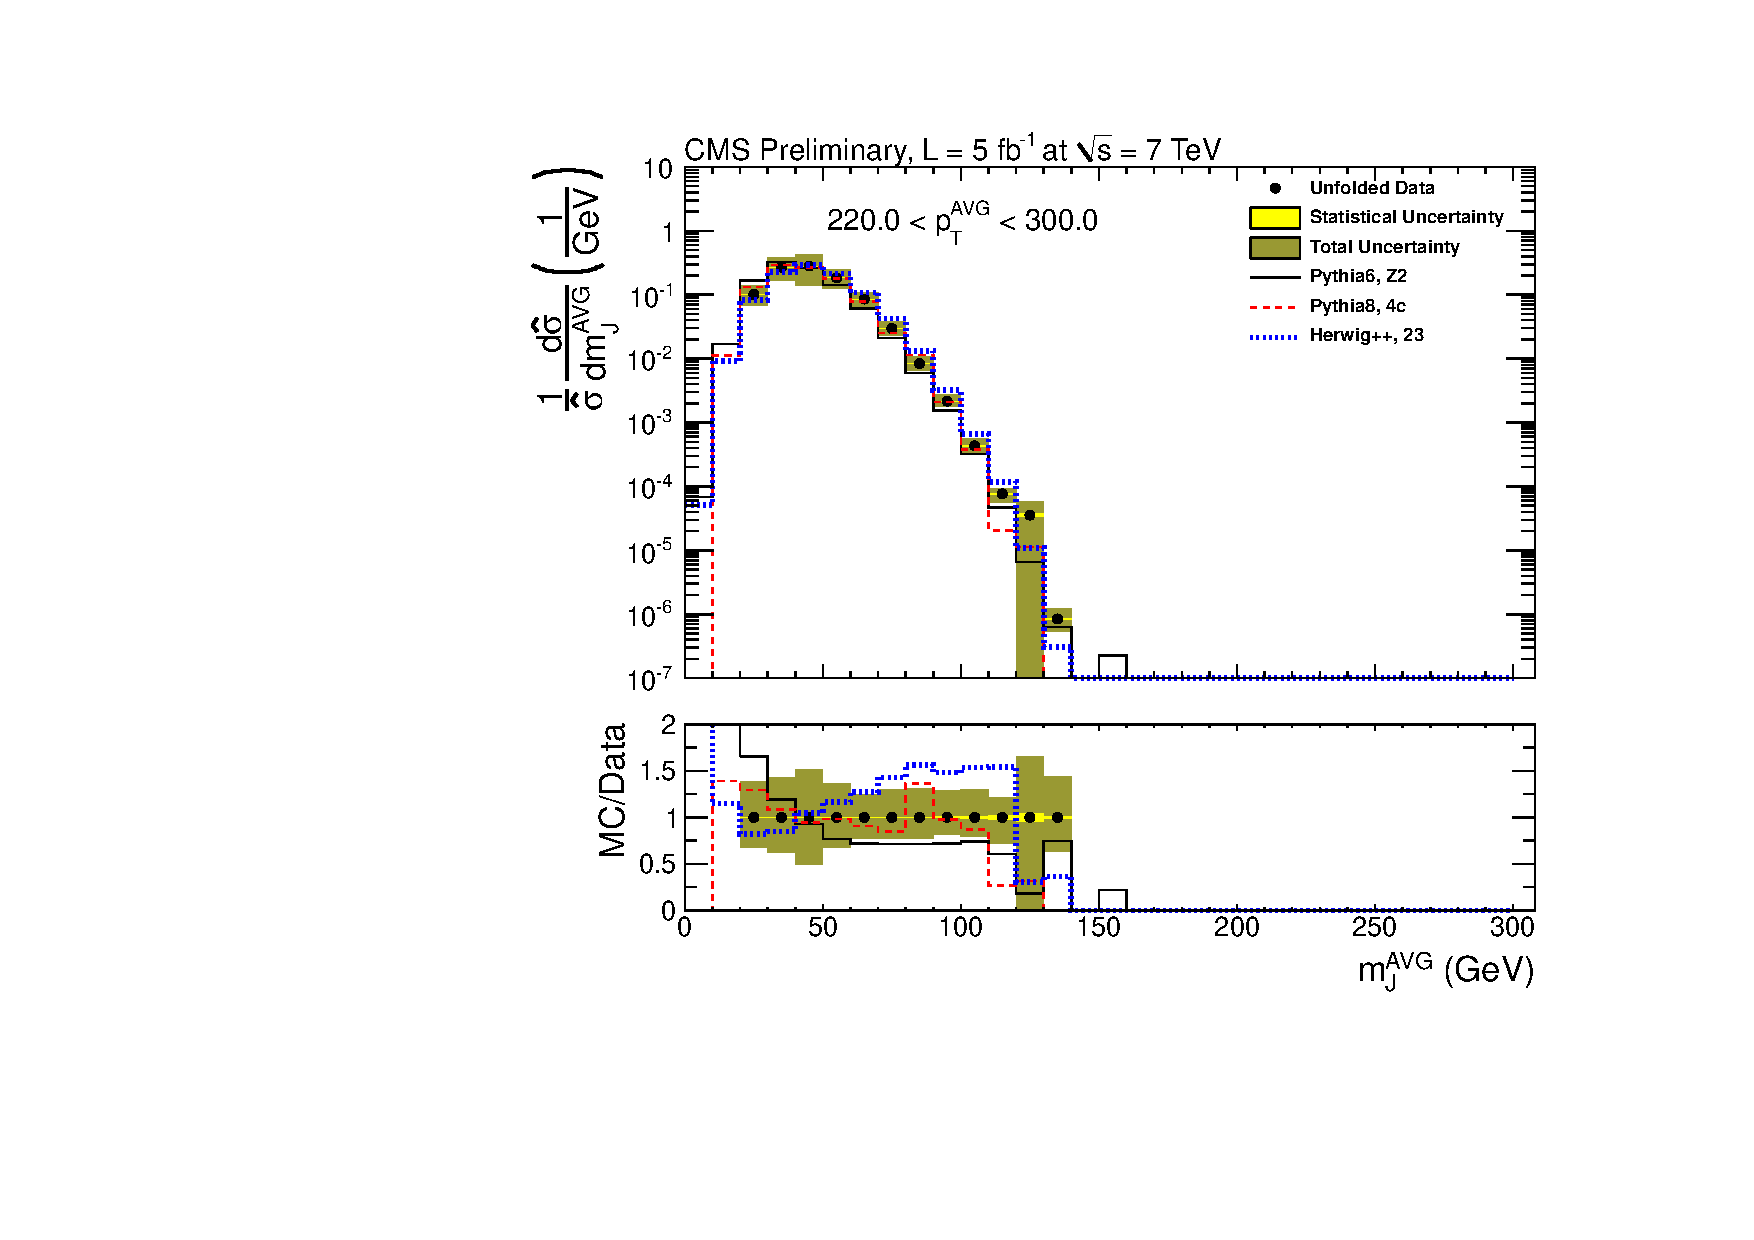
\includegraphics[width=0.95\textwidth]{figs/unfoldedMeasurementDijets_4}
\caption{Unfolded distributions of the jet mass for AK7 jets,
for $220.0 < \pt^{AVG} < 300.0$ \GeVc. The data are shown in black
points. 
The statistical uncertainty is shown in light yellow (light gray), and the statistical plus systematic uncertainty is shown in dark yellow (dark gray).
The simulated distribution from \PYTHIA is shown in solid black, 
the from \PYTHIAEIGHT in dashed red, and from \HERWIG in dotted blue. 
The bottom frame shows the ratio of the true distribution from
the simulation divided by the unfolded distribution, along with
the uncertainties in the unfolded distribution. 
\label{figs:unfoldedMeasurementDijets_4}}
\end{figure}



\begin{figure}[htbp]
\centering
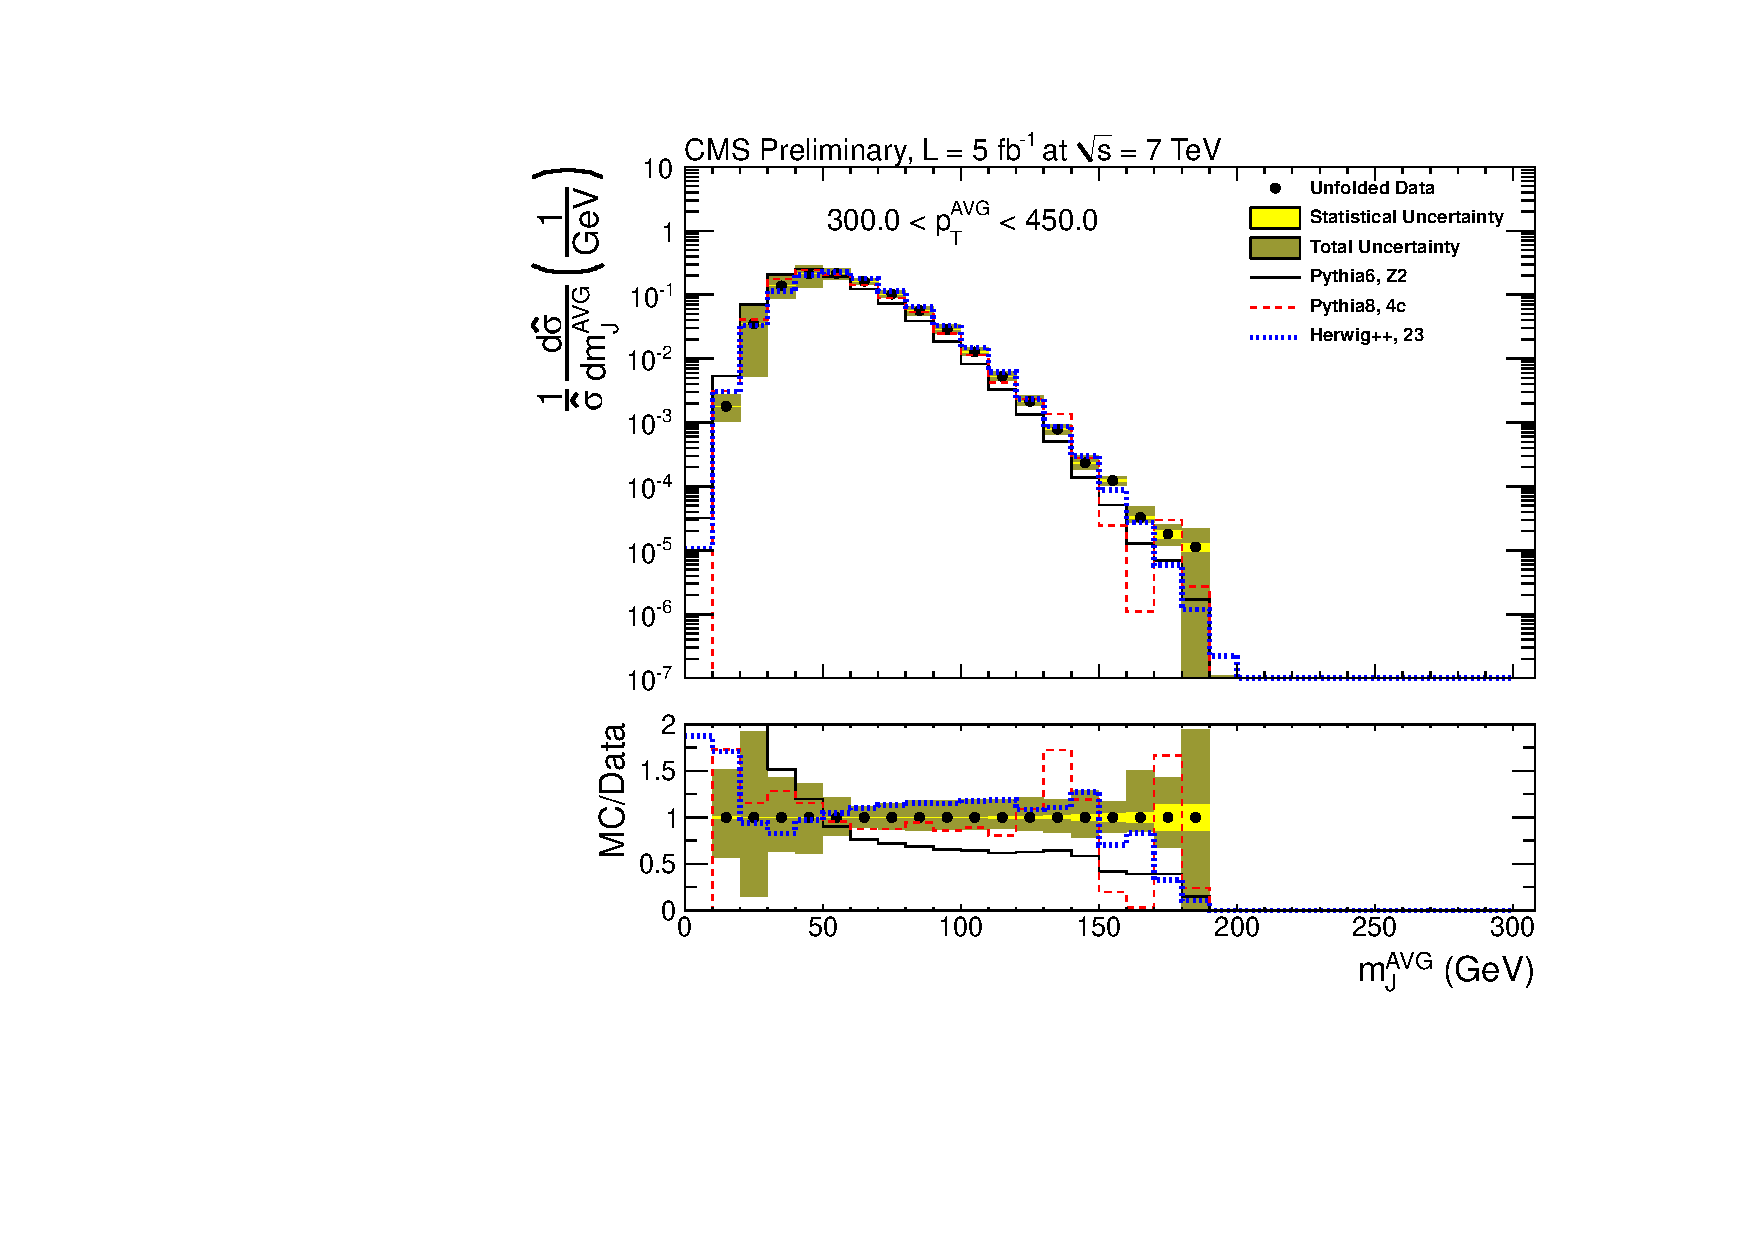
\includegraphics[width=0.95\textwidth]{figs/unfoldedMeasurementDijets_5}
\caption{Unfolded distributions of the jet mass for AK7 jets,
for $300.0 < \pt^{AVG} < 450.0$ \GeVc. The data are shown in black
points. 
The statistical uncertainty is shown in light yellow (light gray), and the statistical plus systematic uncertainty is shown in dark yellow (dark gray).
The simulated distribution from \PYTHIA is shown in solid black, 
the from \PYTHIAEIGHT in dashed red, and from \HERWIG in dotted blue. 
The bottom frame shows the ratio of the true distribution from
the simulation divided by the unfolded distribution, along with
the uncertainties in the unfolded distribution. 
\label{figs:unfoldedMeasurementDijets_5}}
\end{figure}

\fi
%%%%

\ifnpas

\begin{figure}[htbp]
\centering
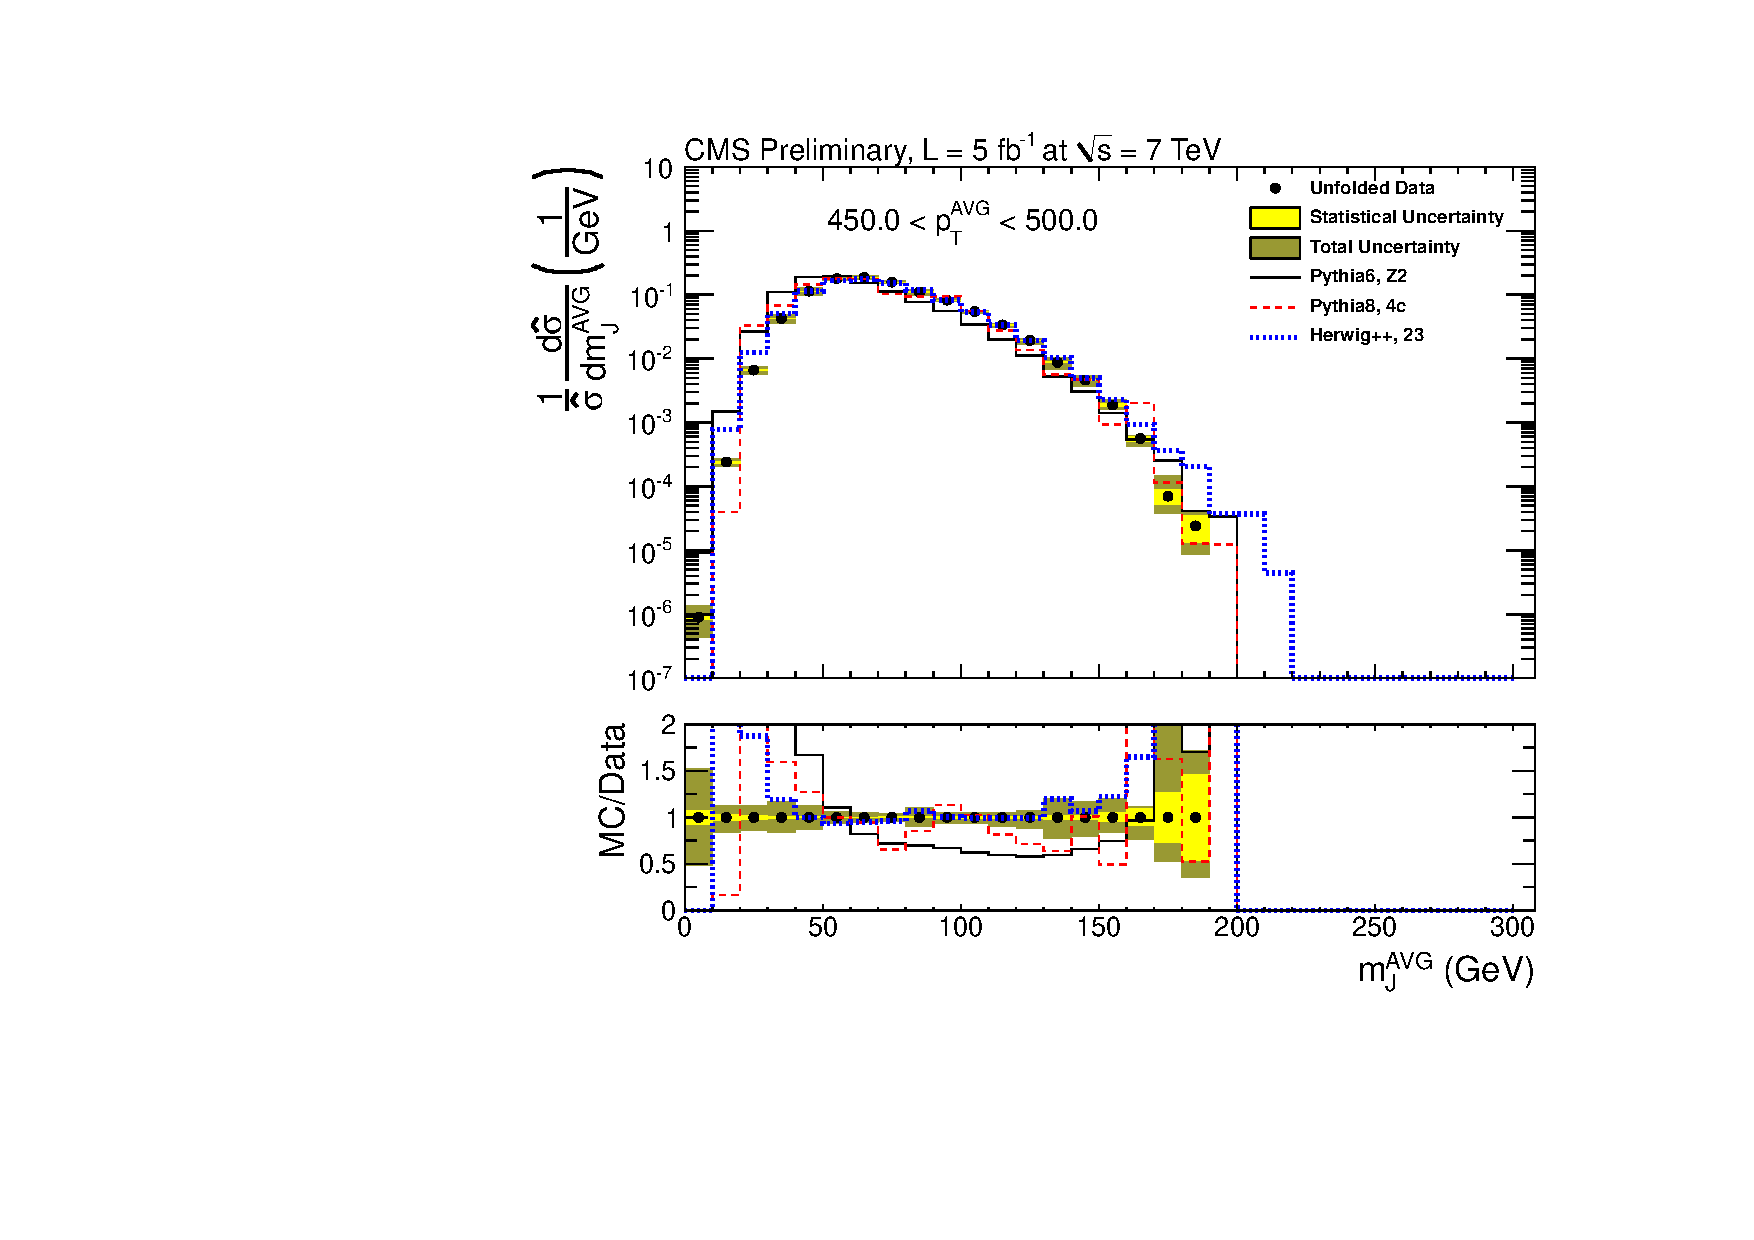
\includegraphics[width=0.95\textwidth]{figs/unfoldedMeasurementDijets_6}
\caption{Unfolded distributions of the jet mass for AK7 jets,
for $450.0 < \pt^{AVG} < 500.0$ \GeVc. The data are shown in black
points. 
The statistical uncertainty is shown in light yellow (light gray), and the statistical plus systematic uncertainty is shown in dark yellow (dark gray).
The simulated distribution from \PYTHIA is shown in solid black, 
the from \PYTHIAEIGHT in dashed red, and from \HERWIG in dotted blue. 
The bottom frame shows the ratio of the true distribution from
the simulation divided by the unfolded distribution, along with
the uncertainties in the unfolded distribution. 
\label{figs:unfoldedMeasurementDijets_6}}
\end{figure}



\begin{figure}[htbp]
\centering
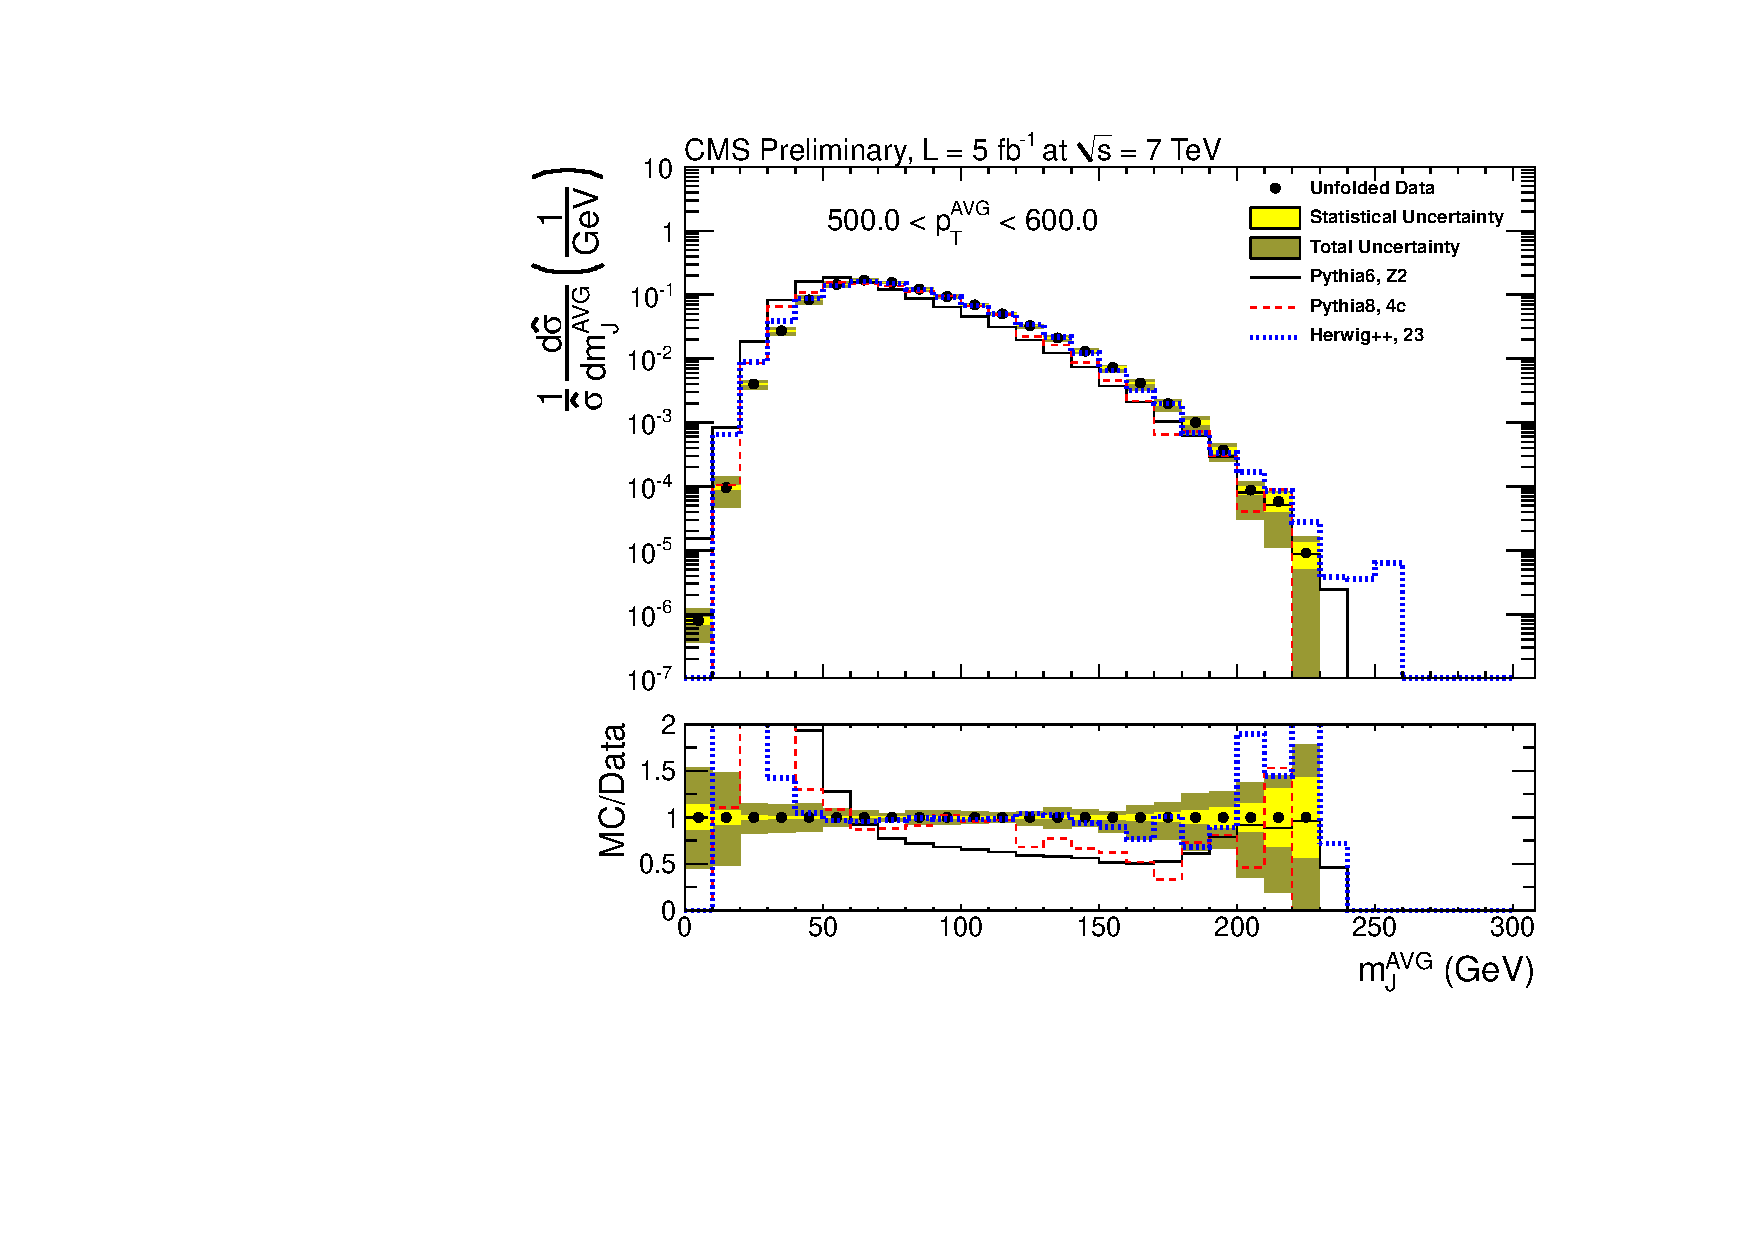
\includegraphics[width=0.95\textwidth]{figs/unfoldedMeasurementDijets_7}
\caption{Unfolded distributions of the jet mass for AK7 jets,
for $500.0 < \pt^{AVG} < 600.0$ \GeVc. The data are shown in black
points. 
The statistical uncertainty is shown in light yellow (light gray), and the statistical plus systematic uncertainty is shown in dark yellow (dark gray).
The simulated distribution from \PYTHIA is shown in solid black, 
the from \PYTHIAEIGHT in dashed red, and from \HERWIG in dotted blue. 
The bottom frame shows the ratio of the true distribution from
the simulation divided by the unfolded distribution, along with
the uncertainties in the unfolded distribution. 
\label{figs:unfoldedMeasurementDijets_7}}
\end{figure}



\begin{figure}[htbp]
\centering
\includegraphics[width=0.95\textwidth]{figs/unfoldedMeasurementDijets_8}
\caption{Unfolded distributions of the jet mass for AK7 jets,
for $600.0 < \pt^{AVG} < 800.0$ \GeVc. The data are shown in black
points. 
The statistical uncertainty is shown in light yellow (light gray), and the statistical plus systematic uncertainty is shown in dark yellow (dark gray).
The simulated distribution from \PYTHIA is shown in solid black, 
the from \PYTHIAEIGHT in dashed red, and from \HERWIG in dotted blue. 
The bottom frame shows the ratio of the true distribution from
the simulation divided by the unfolded distribution, along with
the uncertainties in the unfolded distribution. 
\label{figs:unfoldedMeasurementDijets_8}}
\end{figure}



\begin{figure}[htbp]
\centering
\includegraphics[width=0.95\textwidth]{figs/unfoldedMeasurementDijets_9}
\caption{Unfolded distributions of the jet mass for AK7 jets,
for $800.0 < \pt^{AVG} < 1000.0$ \GeVc. The data are shown in black
points. 
The statistical uncertainty is shown in light yellow (light gray), and the statistical plus systematic uncertainty is shown in dark yellow (dark gray).
The simulated distribution from \PYTHIA is shown in solid black, 
the from \PYTHIAEIGHT in dashed red, and from \HERWIG in dotted blue. 
The bottom frame shows the ratio of the true distribution from
the simulation divided by the unfolded distribution, along with
the uncertainties in the unfolded distribution. 
\label{figs:unfoldedMeasurementDijets_9}}
\end{figure}



\begin{figure}[htbp]
\centering
\includegraphics[width=0.95\textwidth]{figs/unfoldedMeasurementDijets_10}
\caption{Unfolded distributions of the jet mass for AK7 jets,
for $1000.0 < \pt^{AVG} < 1500.0$ \GeVc. The data are shown in black
points. 
The statistical uncertainty is shown in light yellow (light gray), and the statistical plus systematic uncertainty is shown in dark yellow (dark gray).
The simulated distribution from \PYTHIA is shown in solid black, 
the from \PYTHIAEIGHT in dashed red, and from \HERWIG in dotted blue. 
The bottom frame shows the ratio of the true distribution from
the simulation divided by the unfolded distribution, along with
the uncertainties in the unfolded distribution. 
\label{figs:unfoldedMeasurementDijets_10}}
\end{figure}
\fi

\clearpage

\ifnpas
\begin{figure}[htbp]
\centering
\includegraphics[width=0.95\textwidth]{figs/unfoldedMeasurementDijets_1_Filtered}
\caption{Unfolded distributions of the jet mass for AK7 Filtered jets,
for $50.0 < \pt^{AVG} < 125.0$ \GeVc. The data are shown in black
points. 
The statistical uncertainty is shown in light yellow (light gray), and the statistical plus systematic uncertainty is shown in dark yellow (dark gray).
The simulated distribution from \PYTHIA is shown in solid black, 
the from \PYTHIAEIGHT in dashed red, and from \HERWIG in dotted blue. 
The bottom frame shows the ratio of the true distribution from
the simulation divided by the unfolded distribution, along with
the uncertainties in the unfolded distribution. 
\label{figs:unfoldedMeasurementDijets_1_Filtered}}
\end{figure}
\fi


\begin{figure}[htbp]
\centering
\includegraphics[width=0.49\textwidth]{figs/unfoldedMeasurementDijets_2_Filtered}
\includegraphics[width=0.49\textwidth]{figs/unfoldedMeasurementDijets_3_Filtered}
\includegraphics[width=0.49\textwidth]{figs/unfoldedMeasurementDijets_4_Filtered}
\includegraphics[width=0.49\textwidth]{figs/unfoldedMeasurementDijets_5_Filtered}
\caption{Unfolded distributions of the jet mass for AK7 Filtered jets,
for several $\pt^{AVG}$ bins. The data are shown in black
%for $125.0 < \pt^{AVG} < 150.0$ \GeVc. The data are shown in black
points. 
The statistical uncertainty is shown in light yellow (light gray), and the statistical plus systematic uncertainty is shown in dark yellow (dark gray).
The simulated distribution from \PYTHIA is shown in solid black, 
the from \PYTHIAEIGHT in dashed red, and from \HERWIG in dotted blue. 
The bottom frame shows the ratio of the true distribution from
the simulation divided by the unfolded distribution, along with
the uncertainties in the unfolded distribution. 
\label{figs:unfoldedMeasurementDijets_2_Filtered}}
\end{figure}

%%%%%%%
\ifnpas

\begin{figure}[htbp]
\centering
\includegraphics[width=0.95\textwidth]{figs/unfoldedMeasurementDijets_3_Filtered}
\caption{Unfolded distributions of the jet mass for AK7 Filtered jets,
for $150.0 < \pt^{AVG} < 220.0$ \GeVc. The data are shown in black
points. 
The statistical uncertainty is shown in light yellow (light gray), and the statistical plus systematic uncertainty is shown in dark yellow (dark gray).
The simulated distribution from \PYTHIA is shown in solid black, 
the from \PYTHIAEIGHT in dashed red, and from \HERWIG in dotted blue. 
The bottom frame shows the ratio of the true distribution from
the simulation divided by the unfolded distribution, along with
the uncertainties in the unfolded distribution. 
\label{figs:unfoldedMeasurementDijets_3_Filtered}}
\end{figure}



\begin{figure}[htbp]
\centering
\includegraphics[width=0.95\textwidth]{figs/unfoldedMeasurementDijets_4_Filtered}
\caption{Unfolded distributions of the jet mass for AK7 Filtered jets,
for $220.0 < \pt^{AVG} < 300.0$ \GeVc. The data are shown in black
points. 
The statistical uncertainty is shown in light yellow (light gray), and the statistical plus systematic uncertainty is shown in dark yellow (dark gray).
The simulated distribution from \PYTHIA is shown in solid black, 
the from \PYTHIAEIGHT in dashed red, and from \HERWIG in dotted blue. 
The bottom frame shows the ratio of the true distribution from
the simulation divided by the unfolded distribution, along with
the uncertainties in the unfolded distribution. 
\label{figs:unfoldedMeasurementDijets_4_Filtered}}
\end{figure}



\begin{figure}[htbp]
\centering
\includegraphics[width=0.95\textwidth]{figs/unfoldedMeasurementDijets_5_Filtered}
\caption{Unfolded distributions of the jet mass for AK7 Filtered jets,
for $300.0 < \pt^{AVG} < 450.0$ \GeVc. The data are shown in black
points. 
The statistical uncertainty is shown in light yellow (light gray), and the statistical plus systematic uncertainty is shown in dark yellow (dark gray).
The simulated distribution from \PYTHIA is shown in solid black, 
the from \PYTHIAEIGHT in dashed red, and from \HERWIG in dotted blue. 
The bottom frame shows the ratio of the true distribution from
the simulation divided by the unfolded distribution, along with
the uncertainties in the unfolded distribution. 
\label{figs:unfoldedMeasurementDijets_5_Filtered}}
\end{figure}

\fi
%%%%%

\ifnpas

\begin{figure}[htbp]
\centering
\includegraphics[width=0.95\textwidth]{figs/unfoldedMeasurementDijets_6_Filtered}
\caption{Unfolded distributions of the jet mass for AK7 Filtered jets,
for $450.0 < \pt^{AVG} < 500.0$ \GeVc. The data are shown in black
points. 
The statistical uncertainty is shown in light yellow (light gray), and the statistical plus systematic uncertainty is shown in dark yellow (dark gray).
The simulated distribution from \PYTHIA is shown in solid black, 
the from \PYTHIAEIGHT in dashed red, and from \HERWIG in dotted blue. 
The bottom frame shows the ratio of the true distribution from
the simulation divided by the unfolded distribution, along with
the uncertainties in the unfolded distribution. 
\label{figs:unfoldedMeasurementDijets_6_Filtered}}
\end{figure}



\begin{figure}[htbp]
\centering
\includegraphics[width=0.95\textwidth]{figs/unfoldedMeasurementDijets_7_Filtered}
\caption{Unfolded distributions of the jet mass for AK7 Filtered jets,
for $500.0 < \pt^{AVG} < 600.0$ \GeVc. The data are shown in black
points. 
The statistical uncertainty is shown in light yellow (light gray), and the statistical plus systematic uncertainty is shown in dark yellow (dark gray).
The simulated distribution from \PYTHIA is shown in solid black, 
the from \PYTHIAEIGHT in dashed red, and from \HERWIG in dotted blue. 
The bottom frame shows the ratio of the true distribution from
the simulation divided by the unfolded distribution, along with
the uncertainties in the unfolded distribution. 
\label{figs:unfoldedMeasurementDijets_7_Filtered}}
\end{figure}



\begin{figure}[htbp]
\centering
\includegraphics[width=0.95\textwidth]{figs/unfoldedMeasurementDijets_8_Filtered}
\caption{Unfolded distributions of the jet mass for AK7 Filtered jets,
for $600.0 < \pt^{AVG} < 800.0$ \GeVc. The data are shown in black
points. 
The statistical uncertainty is shown in light yellow (light gray), and the statistical plus systematic uncertainty is shown in dark yellow (dark gray).
The simulated distribution from \PYTHIA is shown in solid black, 
the from \PYTHIAEIGHT in dashed red, and from \HERWIG in dotted blue. 
The bottom frame shows the ratio of the true distribution from
the simulation divided by the unfolded distribution, along with
the uncertainties in the unfolded distribution. 
\label{figs:unfoldedMeasurementDijets_8_Filtered}}
\end{figure}



\begin{figure}[htbp]
\centering
\includegraphics[width=0.95\textwidth]{figs/unfoldedMeasurementDijets_9_Filtered}
\caption{Unfolded distributions of the jet mass for AK7 Filtered jets,
for $800.0 < \pt^{AVG} < 1000.0$ \GeVc. The data are shown in black
points. 
The statistical uncertainty is shown in light yellow (light gray), and the statistical plus systematic uncertainty is shown in dark yellow (dark gray).
The simulated distribution from \PYTHIA is shown in solid black, 
the from \PYTHIAEIGHT in dashed red, and from \HERWIG in dotted blue. 
The bottom frame shows the ratio of the true distribution from
the simulation divided by the unfolded distribution, along with
the uncertainties in the unfolded distribution. 
\label{figs:unfoldedMeasurementDijets_9_Filtered}}
\end{figure}



\begin{figure}[htbp]
\centering
\includegraphics[width=0.95\textwidth]{figs/unfoldedMeasurementDijets_10_Filtered}
\caption{Unfolded distributions of the jet mass for AK7 Filtered jets,
for $1000.0 < \pt^{AVG} < 1500.0$ \GeVc. The data are shown in black
points. 
The statistical uncertainty is shown in light yellow (light gray), and the statistical plus systematic uncertainty is shown in dark yellow (dark gray).
The simulated distribution from \PYTHIA is shown in solid black, 
the from \PYTHIAEIGHT in dashed red, and from \HERWIG in dotted blue. 
The bottom frame shows the ratio of the true distribution from
the simulation divided by the unfolded distribution, along with
the uncertainties in the unfolded distribution. 
\label{figs:unfoldedMeasurementDijets_10_Filtered}}
\end{figure}
\fi

\clearpage

\ifnpas

\begin{figure}[htbp]
\centering
\includegraphics[width=0.95\textwidth]{figs/unfoldedMeasurementDijets_1_Trimmed}
\caption{Unfolded distributions of the jet mass for AK7 Trimmed jets,
for $50.0 < \pt^{AVG} < 125.0$ \GeVc. The data are shown in black
points. 
The statistical uncertainty is shown in light yellow (light gray), and the statistical plus systematic uncertainty is shown in dark yellow (dark gray).
The simulated distribution from \PYTHIA is shown in solid black, 
the from \PYTHIAEIGHT in dashed red, and from \HERWIG in dotted blue. 
The bottom frame shows the ratio of the true distribution from
the simulation divided by the unfolded distribution, along with
the uncertainties in the unfolded distribution. 
\label{figs:unfoldedMeasurementDijets_1_Trimmed}}
\end{figure}

\fi

\begin{figure}[htbp]
\centering
\includegraphics[width=0.49\textwidth]{figs/unfoldedMeasurementDijets_2_Trimmed}
\includegraphics[width=0.49\textwidth]{figs/unfoldedMeasurementDijets_3_Trimmed}
\includegraphics[width=0.49\textwidth]{figs/unfoldedMeasurementDijets_4_Trimmed}
\includegraphics[width=0.49\textwidth]{figs/unfoldedMeasurementDijets_5_Trimmed}
\caption{Unfolded distributions of the jet mass for AK7 Trimmed jets,
%for $125.0 < \pt^{AVG} < 150.0$ \GeVc. The data are shown in black
for several $\pt^{AVG}$ bins. The data are shown in black
points. 
The statistical uncertainty is shown in light yellow (light gray), and the statistical plus systematic uncertainty is shown in dark yellow (dark gray).
The simulated distribution from \PYTHIA is shown in solid black, 
the from \PYTHIAEIGHT in dashed red, and from \HERWIG in dotted blue. 
The bottom frame shows the ratio of the true distribution from
the simulation divided by the unfolded distribution, along with
the uncertainties in the unfolded distribution. 
\label{figs:unfoldedMeasurementDijets_2_Trimmed}}
\end{figure}


%%%%%%
\ifnpas

\begin{figure}[htbp]
\centering
\includegraphics[width=0.95\textwidth]{figs/unfoldedMeasurementDijets_3_Trimmed}
\caption{Unfolded distributions of the jet mass for AK7 Trimmed jets,
for $150.0 < \pt^{AVG} < 220.0$ \GeVc. The data are shown in black
points. 
The statistical uncertainty is shown in light yellow (light gray), and the statistical plus systematic uncertainty is shown in dark yellow (dark gray).
The simulated distribution from \PYTHIA is shown in solid black, 
the from \PYTHIAEIGHT in dashed red, and from \HERWIG in dotted blue. 
The bottom frame shows the ratio of the true distribution from
the simulation divided by the unfolded distribution, along with
the uncertainties in the unfolded distribution. 
\label{figs:unfoldedMeasurementDijets_3_Trimmed}}
\end{figure}



\begin{figure}[htbp]
\centering
\includegraphics[width=0.95\textwidth]{figs/unfoldedMeasurementDijets_4_Trimmed}
\caption{Unfolded distributions of the jet mass for AK7 Trimmed jets,
for $220.0 < \pt^{AVG} < 300.0$ \GeVc. The data are shown in black
points. 
The statistical uncertainty is shown in light yellow (light gray), and the statistical plus systematic uncertainty is shown in dark yellow (dark gray).
The simulated distribution from \PYTHIA is shown in solid black, 
the from \PYTHIAEIGHT in dashed red, and from \HERWIG in dotted blue. 
The bottom frame shows the ratio of the true distribution from
the simulation divided by the unfolded distribution, along with
the uncertainties in the unfolded distribution. 
\label{figs:unfoldedMeasurementDijets_4_Trimmed}}
\end{figure}



\begin{figure}[htbp]
\centering
\includegraphics[width=0.95\textwidth]{figs/unfoldedMeasurementDijets_5_Trimmed}
\caption{Unfolded distributions of the jet mass for AK7 Trimmed jets,
for $300.0 < \pt^{AVG} < 450.0$ \GeVc. The data are shown in black
points. 
The statistical uncertainty is shown in light yellow (light gray), and the statistical plus systematic uncertainty is shown in dark yellow (dark gray).
The simulated distribution from \PYTHIA is shown in solid black, 
the from \PYTHIAEIGHT in dashed red, and from \HERWIG in dotted blue. 
The bottom frame shows the ratio of the true distribution from
the simulation divided by the unfolded distribution, along with
the uncertainties in the unfolded distribution. 
\label{figs:unfoldedMeasurementDijets_5_Trimmed}}
\end{figure}

\fi
%%%%%%%%%%


\ifnpas

\begin{figure}[htbp]
\centering
\includegraphics[width=0.95\textwidth]{figs/unfoldedMeasurementDijets_6_Trimmed}
\caption{Unfolded distributions of the jet mass for AK7 Trimmed jets,
for $450.0 < \pt^{AVG} < 500.0$ \GeVc. The data are shown in black
points. 
The statistical uncertainty is shown in light yellow (light gray), and the statistical plus systematic uncertainty is shown in dark yellow (dark gray).
The simulated distribution from \PYTHIA is shown in solid black, 
the from \PYTHIAEIGHT in dashed red, and from \HERWIG in dotted blue. 
The bottom frame shows the ratio of the true distribution from
the simulation divided by the unfolded distribution, along with
the uncertainties in the unfolded distribution. 
\label{figs:unfoldedMeasurementDijets_6_Trimmed}}
\end{figure}



\begin{figure}[htbp]
\centering
\includegraphics[width=0.95\textwidth]{figs/unfoldedMeasurementDijets_7_Trimmed}
\caption{Unfolded distributions of the jet mass for AK7 Trimmed jets,
for $500.0 < \pt^{AVG} < 600.0$ \GeVc. The data are shown in black
points. 
The statistical uncertainty is shown in light yellow (light gray), and the statistical plus systematic uncertainty is shown in dark yellow (dark gray).
The simulated distribution from \PYTHIA is shown in solid black, 
the from \PYTHIAEIGHT in dashed red, and from \HERWIG in dotted blue. 
The bottom frame shows the ratio of the true distribution from
the simulation divided by the unfolded distribution, along with
the uncertainties in the unfolded distribution. 
\label{figs:unfoldedMeasurementDijets_7_Trimmed}}
\end{figure}



\begin{figure}[htbp]
\centering
\includegraphics[width=0.95\textwidth]{figs/unfoldedMeasurementDijets_8_Trimmed}
\caption{Unfolded distributions of the jet mass for AK7 Trimmed jets,
for $600.0 < \pt^{AVG} < 800.0$ \GeVc. The data are shown in black
points. 
The statistical uncertainty is shown in light yellow (light gray), and the statistical plus systematic uncertainty is shown in dark yellow (dark gray).
The simulated distribution from \PYTHIA is shown in solid black, 
the from \PYTHIAEIGHT in dashed red, and from \HERWIG in dotted blue. 
The bottom frame shows the ratio of the true distribution from
the simulation divided by the unfolded distribution, along with
the uncertainties in the unfolded distribution. 
\label{figs:unfoldedMeasurementDijets_8_Trimmed}}
\end{figure}



\begin{figure}[htbp]
\centering
\includegraphics[width=0.95\textwidth]{figs/unfoldedMeasurementDijets_9_Trimmed}
\caption{Unfolded distributions of the jet mass for AK7 Trimmed jets,
for $800.0 < \pt^{AVG} < 1000.0$ \GeVc. The data are shown in black
points. 
The statistical uncertainty is shown in light yellow (light gray), and the statistical plus systematic uncertainty is shown in dark yellow (dark gray).
The simulated distribution from \PYTHIA is shown in solid black, 
the from \PYTHIAEIGHT in dashed red, and from \HERWIG in dotted blue. 
The bottom frame shows the ratio of the true distribution from
the simulation divided by the unfolded distribution, along with
the uncertainties in the unfolded distribution. 
\label{figs:unfoldedMeasurementDijets_9_Trimmed}}
\end{figure}



\begin{figure}[htbp]
\centering
\includegraphics[width=0.95\textwidth]{figs/unfoldedMeasurementDijets_10_Trimmed}
\caption{Unfolded distributions of the jet mass for AK7 Trimmed jets,
for $1000.0 < \pt^{AVG} < 1500.0$ \GeVc. The data are shown in black
points. 
The statistical uncertainty is shown in light yellow (light gray), and the statistical plus systematic uncertainty is shown in dark yellow (dark gray).
The simulated distribution from \PYTHIA is shown in solid black, 
the from \PYTHIAEIGHT in dashed red, and from \HERWIG in dotted blue. 
The bottom frame shows the ratio of the true distribution from
the simulation divided by the unfolded distribution, along with
the uncertainties in the unfolded distribution. 
\label{figs:unfoldedMeasurementDijets_10_Trimmed}}
\end{figure}

\fi

\clearpage


\ifnpas
\begin{figure}[htbp]
\centering
\includegraphics[width=0.95\textwidth]{figs/unfoldedMeasurementDijets_1_Pruned}
\caption{Unfolded distributions of the jet mass for AK7 Pruned jets,
for $50.0 < \pt^{AVG} < 125.0$ \GeVc. The data are shown in black
points. 
The statistical uncertainty is shown in light yellow (light gray), and the statistical plus systematic uncertainty is shown in dark yellow (dark gray).
The simulated distribution from \PYTHIA is shown in solid black, 
the from \PYTHIAEIGHT in dashed red, and from \HERWIG in dotted blue. 
The bottom frame shows the ratio of the true distribution from
the simulation divided by the unfolded distribution, along with
the uncertainties in the unfolded distribution. 
\label{figs:unfoldedMeasurementDijets_1_Pruned}}
\end{figure}

\fi

\begin{figure}[htbp]
\centering
\includegraphics[width=0.49\textwidth]{figs/unfoldedMeasurementDijets_2_Pruned}
\includegraphics[width=0.49\textwidth]{figs/unfoldedMeasurementDijets_3_Pruned}
\includegraphics[width=0.49\textwidth]{figs/unfoldedMeasurementDijets_4_Pruned}
\includegraphics[width=0.49\textwidth]{figs/unfoldedMeasurementDijets_5_Pruned}
\caption{Unfolded distributions of the jet mass for AK7 Pruned jets,
%for $125.0 < \pt^{AVG} < 150.0$ \GeVc. The data are shown in black
for several $\pt^{AVG}$ bins. The data are shown in black
points. 
The statistical uncertainty is shown in light yellow (light gray), and the statistical plus systematic uncertainty is shown in dark yellow (dark gray).
The simulated distribution from \PYTHIA is shown in solid black, 
the from \PYTHIAEIGHT in dashed red, and from \HERWIG in dotted blue. 
The bottom frame shows the ratio of the true distribution from
the simulation divided by the unfolded distribution, along with
the uncertainties in the unfolded distribution. 
\label{figs:unfoldedMeasurementDijets_2_Pruned}}
\end{figure}

%%%%%%%%%%%%%%
\ifnpas

\begin{figure}[htbp]
\centering
\includegraphics[width=0.95\textwidth]{figs/unfoldedMeasurementDijets_3_Pruned}
\caption{Unfolded distributions of the jet mass for AK7 Pruned jets,
for $150.0 < \pt^{AVG} < 220.0$ \GeVc. The data are shown in black
points. 
The statistical uncertainty is shown in light yellow (light gray), and the statistical plus systematic uncertainty is shown in dark yellow (dark gray).
The simulated distribution from \PYTHIA is shown in solid black, 
the from \PYTHIAEIGHT in dashed red, and from \HERWIG in dotted blue. 
The bottom frame shows the ratio of the true distribution from
the simulation divided by the unfolded distribution, along with
the uncertainties in the unfolded distribution. 
\label{figs:unfoldedMeasurementDijets_3_Pruned}}
\end{figure}



\begin{figure}[htbp]
\centering
\includegraphics[width=0.95\textwidth]{figs/unfoldedMeasurementDijets_4_Pruned}
\caption{Unfolded distributions of the jet mass for AK7 Pruned jets,
for $220.0 < \pt^{AVG} < 300.0$ \GeVc. The data are shown in black
points. 
The statistical uncertainty is shown in light yellow (light gray), and the statistical plus systematic uncertainty is shown in dark yellow (dark gray).
The simulated distribution from \PYTHIA is shown in solid black, 
the from \PYTHIAEIGHT in dashed red, and from \HERWIG in dotted blue. 
The bottom frame shows the ratio of the true distribution from
the simulation divided by the unfolded distribution, along with
the uncertainties in the unfolded distribution. 
\label{figs:unfoldedMeasurementDijets_4_Pruned}}
\end{figure}



\begin{figure}[htbp]
\centering
\includegraphics[width=0.95\textwidth]{figs/unfoldedMeasurementDijets_5_Pruned}
\caption{Unfolded distributions of the jet mass for AK7 Pruned jets,
for $300.0 < \pt^{AVG} < 450.0$ \GeVc. The data are shown in black
points. 
The statistical uncertainty is shown in light yellow (light gray), and the statistical plus systematic uncertainty is shown in dark yellow (dark gray).
The simulated distribution from \PYTHIA is shown in solid black, 
the from \PYTHIAEIGHT in dashed red, and from \HERWIG in dotted blue. 
The bottom frame shows the ratio of the true distribution from
the simulation divided by the unfolded distribution, along with
the uncertainties in the unfolded distribution. 
\label{figs:unfoldedMeasurementDijets_5_Pruned}}
\end{figure}

\fi
%%%%%%%%%%%%%%%

\ifnpas


\begin{figure}[htbp]
\centering
\includegraphics[width=0.95\textwidth]{figs/unfoldedMeasurementDijets_6_Pruned}
\caption{Unfolded distributions of the jet mass for AK7 Pruned jets,
for $450.0 < \pt^{AVG} < 500.0$ \GeVc. The data are shown in black
points. 
The statistical uncertainty is shown in light yellow (light gray), and the statistical plus systematic uncertainty is shown in dark yellow (dark gray).
The simulated distribution from \PYTHIA is shown in solid black, 
the from \PYTHIAEIGHT in dashed red, and from \HERWIG in dotted blue. 
The bottom frame shows the ratio of the true distribution from
the simulation divided by the unfolded distribution, along with
the uncertainties in the unfolded distribution. 
\label{figs:unfoldedMeasurementDijets_6_Pruned}}
\end{figure}



\begin{figure}[htbp]
\centering
\includegraphics[width=0.95\textwidth]{figs/unfoldedMeasurementDijets_7_Pruned}
\caption{Unfolded distributions of the jet mass for AK7 Pruned jets,
for $500.0 < \pt^{AVG} < 600.0$ \GeVc. The data are shown in black
points. 
The statistical uncertainty is shown in light yellow (light gray), and the statistical plus systematic uncertainty is shown in dark yellow (dark gray).
The simulated distribution from \PYTHIA is shown in solid black, 
the from \PYTHIAEIGHT in dashed red, and from \HERWIG in dotted blue. 
The bottom frame shows the ratio of the true distribution from
the simulation divided by the unfolded distribution, along with
the uncertainties in the unfolded distribution. 
\label{figs:unfoldedMeasurementDijets_7_Pruned}}
\end{figure}



\begin{figure}[htbp]
\centering
\includegraphics[width=0.95\textwidth]{figs/unfoldedMeasurementDijets_8_Pruned}
\caption{Unfolded distributions of the jet mass for AK7 Pruned jets,
for $600.0 < \pt^{AVG} < 800.0$ \GeVc. The data are shown in black
points. 
The statistical uncertainty is shown in light yellow (light gray), and the statistical plus systematic uncertainty is shown in dark yellow (dark gray).
The simulated distribution from \PYTHIA is shown in solid black, 
the from \PYTHIAEIGHT in dashed red, and from \HERWIG in dotted blue. 
The bottom frame shows the ratio of the true distribution from
the simulation divided by the unfolded distribution, along with
the uncertainties in the unfolded distribution. 
\label{figs:unfoldedMeasurementDijets_8_Pruned}}
\end{figure}



\begin{figure}[htbp]
\centering
\includegraphics[width=0.95\textwidth]{figs/unfoldedMeasurementDijets_9_Pruned}
\caption{Unfolded distributions of the jet mass for AK7 Pruned jets,
for $800.0 < \pt^{AVG} < 1000.0$ \GeVc. The data are shown in black
points. 
The statistical uncertainty is shown in light yellow (light gray), and the statistical plus systematic uncertainty is shown in dark yellow (dark gray).
The simulated distribution from \PYTHIA is shown in solid black, 
the from \PYTHIAEIGHT in dashed red, and from \HERWIG in dotted blue. 
The bottom frame shows the ratio of the true distribution from
the simulation divided by the unfolded distribution, along with
the uncertainties in the unfolded distribution. 
\label{figs:unfoldedMeasurementDijets_9_Pruned}}
\end{figure}



\begin{figure}[htbp]
\centering
\includegraphics[width=0.95\textwidth]{figs/unfoldedMeasurementDijets_10_Pruned}
\caption{Unfolded distributions of the jet mass for AK7 Pruned jets,
for $1000.0 < \pt^{AVG} < 1500.0$ \GeVc. The data are shown in black
points. 
The statistical uncertainty is shown in light yellow (light gray), and the statistical plus systematic uncertainty is shown in dark yellow (dark gray).
The simulated distribution from \PYTHIA is shown in solid black, 
the from \PYTHIAEIGHT in dashed red, and from \HERWIG in dotted blue. 
The bottom frame shows the ratio of the true distribution from
the simulation divided by the unfolded distribution, along with
the uncertainties in the unfolded distribution. 
\label{figs:unfoldedMeasurementDijets_10_Pruned}}
\end{figure}

\fi

\clearpage
